\documentclass[10pt,a4paper,twoside,headinclude,footinclude,color]{./latex-notes-cls/edoars-notes}
\graphicspath{ {Immagini/} }

\hypersetup{pdfauthor={Edoardo Signorini},
            pdftitle={Introduzione alla teoria dei numeri},
            pdfcreator={Latex with hyperref}}

\begin{document}
%MATERIALE INIZIALE
\begin{frontespizio}
\Preambolo{\usepackage{iwona}}
\Universita{Roma Tre}
\Logo{Immagini/logo}
\Facolta{Matematica}
\Scuola{}
\Piede{A.A. 2015--2016, Semestre II}
\Titoletto{Appunti integrativi}
\Titolo{Introduzione alla teoria dei numeri}
\Sottotitolo{TN410}
\NCandidato{Di}
\Candidato{Edoardo Signorini}
\end{frontespizio}
\tableofcontents

%MATERIALE PRINCIPALE
%!TEX root = ../main.tex
%%%%%%%%%%%%%%%%%%%%%%%%%%%%%%%%%%%%%%%%%
%
%LEZIONE 23/02/2016 - PRIMA SETTIMANA (1)
%
%%%%%%%%%%%%%%%%%%%%%%%%%%%%%%%%%%%%%%%%%
\chapter{Divisione e fattorizzazione}
%%%%%%%%%%%%%%
%INTRODUZIONE%
%%%%%%%%%%%%%%
\section{Introduzione}

\begin{notz}
	In questo corso l'insieme dei numeri naturali \(\N\) è privo dello zero.
\end{notz}

\begin{defn}{Assioma del buon ordinamento}{bo}\index{Assioma!del buon ordinamento}
	Sia \(S\subset\N\) non vuoto, allora:
	\[
		\ex\min S.
	\]
\end{defn}

\begin{oss}
	Il buon ordinamento è equivalente al seguente assioma: Se \(S\subset\Z\) è non vuoto e limitato inferiormente, allora
	\[
		\ex\min S.
	\]
\end{oss}

\begin{teor}{Divisione euclidea}{1.1}\index{Divisione euclidea}
	Siano \(a\in\N,b\in\Z\), allora:
	\[
		\exists!\,q,r\in\Z:b=a\,q+r\text{ e }0\le r<a.
	\]
\end{teor}

\begin{proof}
	Definiamo il seguente insieme
	\[
		S=\Set{b-s\,a | s\in\Z}\subseteq\Z.
	\]
	Sia ora
	\[
		S^+=S\cap\big(\N\cup\{0\}\big),
	\]
	ovvero
	\[
		S^+=\Set{b-s\,a\ge0 | s\in\Z},
	\]
	per cui \(S^+\subseteq\N\cup\{0\}\).
	Sicuramente \(S^+\neq\emptyset\), infatti se \(b\ge0\) avremo
	\[
		b\in S^+;
	\]
	mentre se \(b<0\) segue
	\[
		b-b\,a=b(1-a)\ge 0\graffito{\(b\le 0\) e \((1-a)\le 0\)},
	\]
	per cui
	\[
		b-b\,a\in S^+.
	\]
	Quindi, per il buon ordinamento, \(\ex r=\min S^+\) e supponiamo che
	\[
		r=b-q\,a
	\]
	con \(q\in\Z\). Quindi \(b=a\,q+r\) con \(r\ge 0\), in quanto \(r\in S^+\).
	Se per assurdo \(r\ge a\) si avrebbe
	\[
		r-a\ge 0\iff b-(q+1)a\ge 0,
	\]
	ovvero
	\[
		\begin{split}
			b-(q+1)a\in S^+ & \implies b-(q+1)a\ge r\\
			& \iff r-a\ge r\\
			& \iff a\le 0,
		\end{split}
	\]
	ma ciò è assurdo in quanto \(a\in\N\), per cui
	\[
		0\le r<a.
	\]
	Resta da mostrare l'uncità, supponiamo quindi che esistano \(q',r'\in\Z\) tali che
	\[
		q'a+r'=b=q\,a+r,
	\]
	ne segue
	\[
		\abs{r'-r}=a\,\abs{q'-q}.
	\]
	Se per assurdo \(q'\neq q\) seguirebbe
	\[
		\abs{r'-r}\ge a,
	\]
	ma per ipotesi \(r,r'<a\), da cui
	\[
		\abs{r'-r}<a.
	\]
	Ciò è assurdo, per cui \(q'=q\) e \(r'=r\).
\end{proof}

\begin{defn}{Massimo comun divisore}{MCD}\index{Massimo comun divisore}
	Siano \(a,b\in\N\) e sia \(d\in\N\) tale che:
	\begin{itemize}
		\item \(d\mid a,d\mid b\);
		\item \(\ex k\in\N:k\mid a,k\mid b\implies k\mid d\).
	\end{itemize}
	\(d\) si definisce \emph{massimo comun divisore} di \(a\) e di \(b\).
\end{defn}

\begin{notz}
	Il massimo comun divisore fra \(a\) e \(b\) si indica con \((a,b)\).
\end{notz}

\begin{oss}
	Per definizione si pongono
	\begin{itemize}
		\item \((a,0)=a\);
		\item se \(a,b\in\Z,(a,b)=(\abs{a},\abs{b})\).
	\end{itemize}
\end{oss}

\begin{teor}{Unicità del massimo comun divisore}{1.2}
	Siano \(a,b\in\N\), allora:
	\[
		\exists!\,d=(a,b),
	\]
	e vale l'identità di Bezout, ovvero
	\[
		\ex x,y\in\Z:d=a\,x+b\,y.
	\]
\end{teor}

\begin{proof}
	Definiamo il seguente insieme
	\[
		S=\Set{a\,x+b\,y | x,y\in\Z}\cap\N.
	\]
	Sicuramente \(S\neq\emptyset\) in quanto \(a,b\in S\).
	Sia quindi \(d=\min S\), il quale esiste per il buon ordinamento, per cui
	\[
		\ex x,y\in\Z:d=a\,x+b\,y.
	\]
	Mostriamo che \(d=(a,b)\) tramite la divisione euclidea:
	\[
		\ex q,r\in\Z:a=d\,q+r,
	\]
	con \(0\le r<d\). Per come abbiamo definito \(d\) avremo
	\[
		r=a-d\,q=a(1-q\,x)+b(-q\,y).
	\]
	Se per assurdo \(r>0\) seguirebbe \(r\in S\) che è assurdo per la minimalità di \(d\) in \(S\), da cui
	\[
		r=0\implies a=d\,q\iff d\mid b.
	\]
	Analogamente si mostra che \(d\mid b\).
	Mostriamo che se \(\ex k\in\N:k\mid a\) e \(k\mid b\) allora \(k\mid d\):
	\begin{gather*}
		k\mid a\iff\ex\a\in\Z:k\,\a=a,\\
		k\mid b\iff\ex\b\in\Z:k\,\b=b,
	\end{gather*}
	da cui
	\[
		d=a\,x+b\,y=k(\a\,x+\b\,y),
	\]
	ovvero
	\[
		k\mid d.
	\]
	Infine l'unicità segue banalmente dall'ultima proprietà, infatti se esistesse \(d'\in\N\) che soddisfa le ipotesi del teorema si avrebbe
	\[
		d\mid d'\text{ e }d'\mid d,
	\]
	ovvero
	\[
		d'=d.\qedhere
	\]
\end{proof}

\begin{prop}{Algoritmo di Euclide}{1.3}\index{Algoritmo!di Euclide}
	Dati \(a,b\in\N\), siano \(q_1,\dots,q_{n+1}\) e \(r_1,\dots,r_n\in\Z\) tali che:
	\begin{itemize}
		\item \(r_1>r_2>\dots>r_n\ge 0\);
		\item \(b=a\,q_1+r_1,\\
		      a=r_1 q_2+r_2,\\
		      r_1=r_2 q_3+r_3,\\
		      \dots\\
		      r_{n-2}=r_{n-1}q_n+r_n,\\
		      r_{n-1}=r_n q_{n+1}+0\).
	\end{itemize}
	Allora
	\[
		r_n=(a,b).
	\]
\end{prop}

\begin{proof}
	Mostriamo che se \(a=b\,q+r\) con \(0\le r<b\), allora
	\[
		(a,b)=(b,r).
	\]
	Per definizione
	\[
		(a,b)\mid a,b,
	\]
	per cui \((a,b)\) dividerà ogni combinazione lineare di \(a,b\), in particolare
	\[
		(a,b)\mid a-b\,q=r,
	\]
	per cui \((a,b)\mid b,r\), ovvero
	\[
		(a,b)\mid (b,r).
	\]
	Viceversa
	\[
		(b,r)\mid b,r\implies (b,r)\mid b\,q+r=a,
	\]
	ovvero
	\[
		(b,r)\mid (a,b).
	\]
	Applicando tale osservazione al nostro caso otteniamo
	\[
		\begin{split}
			(a,b) & =(b,r_1)\\
			& =(r_1,r_2)\\
			& =\dots\\
			& =(r_{n-1},r_n),
		\end{split}
	\]
	ma \(r_{n-1}=r_n\,q_{n+1}\) per cui
	\[
		(r_{n-1},r_n)=r_n.\qedhere
	\]
\end{proof}

\begin{oss}
	L'algoritmo di Euclide ci fornisce anche un metodo pratico per trovare l'identità di Bezout, infatti \(\fa j=0,\dots,n\) avremo
	\[
		r_j=x_j a+y_j b,\text{ con }x_j,y_j\in\Z.
	\]
	Infatti, sfruttando le equazioni dell'algoritmo di Euclide, avremo
	\begin{gather*}
		r_0 = a\implies (x_0,y_0)=(1,0);\\
		r_1 = -q_1 a+b\implies (x_1,y_1)=(-q_1,1),
	\end{gather*}
	più in generale
	\[
		\begin{split}
			r_j & =r_{j-2}-q_j r_{j-1}\\
			& =(x_{j-2}a+y_{j-2}b)-q_j(x_{j-1}a+y_{j-1}b)\\
			& =(x_{j-2}-q_j x_{j-1})a+(y_{j-2}-q_j y_{j-1})b.
		\end{split}
	\]
	Quindi
	\[
		\left\{
		\begin{aligned}
			x_0 & =1 \\
			y_0 & =0
		\end{aligned}
		\right. ,\left\{
		\begin{aligned}
			x_1 & =-q_1 \\
			y_1 & =1
		\end{aligned}
		\right. \text{ e }\left\{
		\begin{aligned}
			x_j & =x_{j-2}-q_j x_{j-1} \\
			y_j & =y_{j-2}-q_j y_{j-1}
		\end{aligned}
		\right. .
	\]
\end{oss}

\begin{ese}
	Calcoliamo \((5111,589)\) tramite l'algoritmo di Euclide:
	\begin{gather*}
		5111=8\cdot 589+399,\\
		589=1\cdot 399+190,\\
		399=2\cdot 190+19,\\
		190=10\cdot 19+0.
	\end{gather*}
	Per cui
	\[
		(5111,589)=19.
	\]
\end{ese}

\begin{prop}{Divisore del prodotto di coprimi}{1.4}
	Siano \(a,b\in\N\) tali che \((a,b)=1\).
	Sia \(w\in\N\) tale che \(w\mid a\,b\), allora:
	esistono unici \(u,v\in\N\) tali che
	\begin{itemize}
		\item \(w=u\,v\);
		\item \(u\mid a,v\mid b\).
	\end{itemize}
\end{prop}
%%%%%%%%%%%%%%%%%%%%%%%%%%%%%%%%%%%%%%%%%
%
%LEZIONE 25/02/2016 - PRIMA SETTIMANA (2)
%
%chg:oss. algoritmo di euclide
%%%%%%%%%%%%%%%%%%%%%%%%%%%%%%%%%%%%%%%%%
\begin{proof}
	Poniamo \(u=(a,w)\) e \(v=(b,w)\), dobbiamo verificare che \(u\mid a,v\mid b,u\,v=w\) e che \(u,v\) siano unici:
	\begin{itemize}
		\item Per definizione \(u\) è il massimo comun divisore di \(a\) e \(w\), in particolare risulterà essere divisore di \(a\).
		\item Analogamente \(v\) è un divisore di \(b\).
		\item Per il teorema \ref{th:1.2} sappiamo che
		      \begin{gather*}
			      u=(a,w)\implies u=x_1 a+y_1 w;\\
			      v=(b,w)\implies v=x_2 b+y_2 w,
		      \end{gather*}
		      quindi
		      \[
			      \begin{split}
				      u\,v & =a\,b\,x_1 x_2+w(y_1 x_2 b+x_1 y_1 a+y_1 y_2 w)\graffito{\(w\mid a\,b\)}\\
				      & =w\,K,\text{ con }K\in\Z,
			      \end{split}
		      \]
		      ovvero \(w\mid u\,v\).
		      D'altronde \(1=x\,a+y\,b\), ovvero
		      \[
			      \begin{split}
				      w & =x\,w\,a+y\,w\,b\\
				      & =(w,a)(w,b)S,\text{ con }S\in\Z,
			      \end{split}
		      \]
		      in quanto \(x\,w\,a\) è multiplo di \((w,b)\) e \(y\,w\,b\) è multiplo di \((w,a)\), per cui \(u\,v\mid w\), ovvero
		      \[
			      u\,v=w.
		      \]
		\item Supponiamo che \(u',v'\) siano altri due interi che soddisfano la tesi, in particolare avremo \(u'v'=w\), inoltre \(u'\mid a\) e \(u'\mid w\), da cui
		      \[
			      u'\mid (a,w)=u.
		      \]
		      Se per assurdo \(u'\neq(a,w)\) si avrebbe \(u'<(a,w)\) e, per ragionamenti analoghi ai precedenti, \(v'\leq (b,w)\), da cui
		      \[
			      \begin{split}
				      w & =u'v'\\
				      & <(a,w)(b,w)\\
				      & =w,
			      \end{split}
		      \]
		      ma ciò è assurdo, quindi \(u'=(a,w)=u\). Analogamente si mostra che \(v'=v\).\qedhere
	\end{itemize}
\end{proof}

\begin{oss}
	Se poniamo \(\mathcal{D}(n)=\Set{d\in\N : d\mid n}\), allora, se prendiamo \(a,b\in\N\) tali che \((a,b)=1\), avremo
	\[
		\mathcal{D}(a)\times \mathcal{D}(b)\longleftrightarrow\mathcal{D}(a\,b),
	\]
	dove la corrispondenza biunivoca è determinata da
	\[
		(u,v)\mapsto u\,v,
	\]
	che è biiettiva per la proposizione.
\end{oss}
%%%%%%%
%PRIMI%
%%%%%%%
\section{Primi}

\begin{defn}{Insieme dei divisori}{insiemeDivisori}\index{Insieme!dei divisori}
	Si definisce \emph{l'insieme dei divisori} di \(n\in\N\) come l'insieme dei naturali che dividono \(n\), ovvero
	\[
		\mathcal{D}(n)=\Set{d\in\N : d\mid n}.
	\]
\end{defn}

\begin{defn}{Primo}{primo}\index{Primo}
	Un naturale \(n\in\N\) si definisce \emph{primo} se
	\[
		\big\lvert\mathcal{D}(n)\big\rvert=2.
	\]
\end{defn}

\begin{oss}
	\(1\) non è primo in quanto \(\big\lvert\mathcal{D}(1)\big\rvert=1\).
\end{oss}

\begin{teor}{Divisore primo}{1.5}
	Siano \(a,b\in\N\) e sia \(p\) primo, allora:
	\[
		p\mid a\,b\implies p\mid a\text{ oppure }p\mid b.
	\]
\end{teor}

\begin{proof}
	Supponiamo che \(p\nmid a\), per la primalità di \(p\) avremo che \(p\neq a\), quindi
	\[
		(a,p)=1,
	\]
	per cui esistono \(x,y\in\Z\) tali che \(1=x\,a+y\,p\), da cui
	\[
		\begin{split}
			b & =a\,b\,x+y\,b\,p\\
			& =p\,N,\text{ con }N\in\Z,
		\end{split}
	\]
	ovvero \(p\mid b\).
\end{proof}

\begin{prop}{Divisore primo per una succcessione}{1.6}
	Siano \(a_1,\dots,a_n\in\N\) e sia \(p\) primo, allora:
	\[
		p\mid a_1\cdot\ldots\cdot a_k\implies \ex j=1,\dots,n:p\mid a_j.
	\]
\end{prop}

\begin{proof}
	Basta applicare iterativamente il teorema \ref{th:1.5}, infatti
	\[
		p\mid a_1\cdot\ldots\cdot a_k\implies p\mid a_1\text{ oppure }p\mid a_2\cdot\ldots\cdot a_k,
	\]
	se \(p\nmid a_1\) avremo di conseguenza
	\[
		p\mid a_2\text{ oppure }p\mid a_3\cdot\ldots\cdot a_k.
	\]
	Iterando il procedimento di arriva alla tesi.
\end{proof}

\begin{teor}{Teorema fondamentale dell'aritmetica}{1.7}\index{Teorema!fondamentale dell'aritmetica}
	Sia \(n\in\N\) tale che \(n>1\), allora esistono unici, a meno dell'ordine, \(p_1,\dots,p_r\) primi tali che
	\[
		n=p_1\cdot\ldots\cdot p_r.
	\]
\end{teor}

\begin{proof}
	Dimostriamolo per ampia induzione su \(n\):
	\begin{itemize}
		\item Se \(n=2\) soddisfa banalmente la tesi in quanto \(2\) è primo e si scrive unicamente come se stesso, in quanto non ha altri divisori primi.
		\item Supponiamo che, comunque preso \(2<m<n\), esso sia prodotto di numeri primi.
		      Se \(n\) è primo non ho nulla da dimostrare, supponiamo quindi che non lo sia.

		      \(n\) non primo ammette un divisore non banale, ovvero esiste \(1<n_1<n\) tale che \(n_1\mid n\).
		      Poniamo quindi \(n_2=\frac{n}{n_1}\), di conseguenza \(1<n_2<n\) e
		      \[
			      n=n_1 n_2.
		      \]
		      Per induzione avremo
		      \begin{gather*}
			      n_1=p_1\cdot\ldots\cdot p_r;\\
			      n_2=p_1'\cdot\ldots\cdot p_r',
		      \end{gather*}
		      da cui
		      \[
			      n=p_1\cdot\ldots\cdot p_r p_1'\cdot\ldots\cdot p_r'.
		      \]
	\end{itemize}
	Per dimostrare l'unicità, supponiamo che
	\[
		q_1\cdot\ldots\cdot q_s=n=p_1\cdot\ldots\cdot p_r,
	\]
	dove
	\begin{gather*}
		q_1\le q_2\le\dots\le q_s;\\
		p_1\le p_2\le\dots\le p_r.
	\end{gather*}
	Voglio mostrare che \(r=s\) e che \(q_j=p_j\).
	Ora, per la proposizione \ref{pr:1.6}, \(q_1\mid p_1\cdot\ldots\cdot p_r\) implica
	\[
		\ex j:q_1\mid p_j\implies q_1=p_j,
	\]
	in quanto entrambi primi.
	Analogamente si mostra che
	\[
		\ex i:p_1\mid q_i\implies p_1=q_i.
	\]
	Per cui
	\[
		p_1\le p_j=q_1\le q_i=p_1,
	\]
	ovvero \(p_1=q_1\), da cui
	\[
		q_2\cdot\ldots\cdot q_s=p_2\cdot\ldots\cdot p_r.
	\]
	Iterando ottengo \(s=r\) e \(p_i=q_j\).
\end{proof}

\begin{teor}{Equivalente del teorema fondamentale dell'aritmetica}{1.8}
	Sia \(n\in\N\) tale che \(n>1\), allora esistono unici \(p_1,\dots,p_r\) primi distinti e \(m_1,\dots,m_r\in\N\) tali che
	\[
		n=p_1^{m_1}\cdot\ldots\cdot p_r^{m_r},
	\]
	con \(p_1<\dots<p_r\).
\end{teor}

\begin{proof}
	Segue immediatamente dal teorema fondamentale dell'aritmetica.
\end{proof}
%%%%%%%%%%%%%%%%%%%%%%%%%%%%%%%%%
%PROPRIETA' ELEMENTARI DEI PRIMI%
%%%%%%%%%%%%%%%%%%%%%%%%%%%%%%%%%
\section{Proprietà elementari dei primi}

\begin{teor}{Cardinalità dell'insieme dei numeri primi}{1.9}
	Esistono infiniti numeri primi.
\end{teor}

\begin{proof}
	Sia \(p_1=2\) e supponiamo per assurdo che \(p_1,\dots,p_s\) siano tutti i numeri primi.
	Sia ora
	\[
		N=p_1\cdot\ldots\cdot p_s+1\in\N.
	\]
	Osserviamo che
	\[
		(N,p_j)=1,\,\fa j=1,\dots,s,
	\]
	in quanto
	\[
		1=p_j\frac{1-N}{p_j}+N.
	\]
	Ora, per il teorema fondamentale dell'aritmetica, avremo
	\[
		N=q_1^{m_1}\cdot\ldots\cdot q_r^{m_r},
	\]
	dove \(q_1,\dots,q_r\) sono primi, ma, per quanto osservato a proposito di \((N,p_j)\), avremo che
	\[
		\{q_1,\dots,q_r\}\cap\{p_1,\dots,p_s\}=\emptyset,
	\]
	ma ciò è assurdo, in quanto avevamo supposto che non vi fossero altri numeri primi.
\end{proof}

\begin{oss}
	Esistono numerose dimostrazioni alternative di questo teorema, un'altra strategia è la seguente: consideriamo la seguente sequnza di interi
	\[
		(a_n)_{n\in\N}\subseteq \N^{>1},
	\]
	tale che
	\[
		(a_n,a_m)=1,\,\fa n>m.
	\]
	Allora, se \((l_n)_{n\in\N}\) è una sequenza di numeri primi tali che
	\[
		l_k\mid a_k,
	\]
	si ha che \(\{l_k\}\) sono tutti distinti e sono infiniti.
\end{oss}

\begin{ese}
	Costruiamo la sequenza \(a_n\) come segue:
	\begin{align*}
		a_1 & =2,                           \\
		a_2 & =2+1=3,                       \\
		a_3 & =2\cdot 3+1=7,                \\
		a_4 & =2\cdot3\cdot7+1=43,          \\
		a_5 & =2\cdot3\cdot7\cdot43+1=1807, \\
		\dots                               \\
		a_n & =(a_{n-1}-1)a_{n-1}+1,
	\end{align*}
	allora \(a_n\) soddisfa il criterio.
\end{ese}

\begin{ese}
	Mostriamo che la sequenza \((2^{2^k}+1)_{k\in\N}\) soddisfa il criterio.
	Per farlo, verifichiamo che
	\[
		2^{2^n}-1=3\prod_{j=1}^{n-1}2^{2^j}+1,
	\]
	è sufficiente sviluppare \(2^{2^n}-1\) come differenza di quadrati:
	\[
		\begin{split}
			2^{2^n}-1 & =\big(2^{2^{n-1}}+1\big)\big(2^{2^{n-1}}-1\big)\\
			& =\big(2^{2^{n-1}}+1\big)\big(2^{2^{n-2}}+1\big)\big(2^{2^{n-2}}-1\big)\\
			& =\left(\prod_{j=1}^{n-1}2^{2^j}+1\right)\big(2^2-1\big)\\
			& =3\prod_{j=1}^{n-1}2^{2^j}+1.
		\end{split}
	\]
	Affinchè il criterio sia valido, dobbiamo mostrare che tutti gli elementi della sequnza sono coprimi.
	Se per assurdo
	\[
		p\mid (2^{2^k}+1,2^{2^j}+1),\text{ con }k<t,
	\]
	allora, in particolare, \(p\mid(2^{2^k}+1)\) e, per linearità, dividerebbe anche ogni suo multiplo, da cui
	\[
		p\mid 3\prod_{j=1}^{t-1}2^{2^j}+1.
	\]
	Ma, per quanto mostrato
	\[
		3\prod_{j=1}^{t-1}2^{2^j}+1=2^{2^t}-1,
	\]
	ovvero
	\[
		p\mid (2^{2^t}-1).
	\]
	Quindi, ancora per linearità
	\[
		p\mid (2^{2^t}+1)-(2^{2^t}-1)=2,
	\]
	da cui, per la primalità di \(p\), segue \(p=2\).
	Ma ciò è assurdo in quanto \(p\mid 2^{2^k}+1\) che è dispari.
	Quindi la successione soddisfa il criterio.
\end{ese}
%%%%%%%%%%%%%%%%%%%%%%%%%%%%%%%%%%%%%%%
%ALCUNI RISULTATI E PROBLEMI SUI PRIMI%
%%%%%%%%%%%%%%%%%%%%%%%%%%%%%%%%%%%%%%%
\section{Alcuni risultati e problemi sui primi}

\begin{defn}{Funzione enumerativa dei primi}{funzionePi}\index{Funzione!enumerativa dei primi}
	Si definisce \emph{funzione enumerativa dei primi} l'applicazione che associa ad ogni numero naturale \(n\) il numero dei primi non superiori ad \(n\), ovvero
	\[
		\p(n)=\big\lvert\{p\le n\}\big\rvert.
	\]
\end{defn}

\begin{ese}
	Alcuni valori della funzione \(\p\):
	\begin{itemize}
		\item \(\p(1)=0\);
		\item \(\p(2)=1\);
		\item \(\p(100)=25\).
	\end{itemize}
\end{ese}

\begin{teor}{Teorema dei numeri primi}{teorPrimi}\index{Teorema!dei numeri primi}
	Sia \(\p\) la funzione enumerativa dei numeri primi, allora:
	\[
		\p(x)\sim\frac{x}{\ln x}.
	\]
\end{teor}

\begin{proof}
	Si rimanda ad un corso superiore di teoria dei numeri.
\end{proof}

\begin{oss}
	La dimostrazione sfrutta l'anialisi complessa attraverso lo studio della funzione zeta di Riemann
	\[
		\z(s)=\sum_{n=1}^{\infty}\frac{1}{n^s},
	\]
	la quale è una funzione differenziabile (olomorfa) nella regione
	\[
		\Set{s\in\C | \Re(s)>1}\subseteq\C.
	\]
\end{oss}

\begin{prop}{Stima della funzione enumerativa dei numeri primi}{stimaPrimi}
	Sia \(\p\) la funzione enumerativa dei numeri primi, allora:
	\[
		\p(x)\ge\log_2(\log_2 x)-1,
	\]
	per \(x\ge 2\).
\end{prop}

\begin{proof}
	Sia \(k=\max\{j:2^{2^j}+1\le x\}\), mostriamo che
	\[
		\p(x)\ge k.
	\]
	Infatti
	\[
		[1,x]\cap\{2^{2^j}+1:j\in\N\}=\{5,17,\dots,2^{2^k}+1\},
	\]
	ovvero
	\[
		\#\big([1,x]\cap\{2^{2^j}+1:j\in\N\}\big)=k,
	\]
	da cui
	\[
		\p(x)=\#\{p\text{ primo }:p\le x\}\ge\#\big([1,x]\cap\{2^{2^j}+1:j\in\N\}\big)=k.
	\]
	Infine, per ipotesi, \(2^{2^{k+1}}+1>x\) da cui \(2^{2^{k+1}}\ge x\), ovvero
	\[
		k+1\ge \log_2(\log_2 x),
	\]
	quindi
	\[
		\p(x)\ge k\ge \log_2(\log_2 x)-1.\qedhere
	\]
\end{proof}
%%%%%%%%%%%%%%%%%%%%%%%%%%%%%%%%%%%%%%%%%
%
%LEZIONE 26/02/2016 - PRIMA SETTIMANA (3)
%
%%%%%%%%%%%%%%%%%%%%%%%%%%%%%%%%%%%%%%%%%
\begin{teor}{di Gauss}{teorGauss}\index{Teorema!di Gauss}
	Sia \(\p\) la funzione enumerativa dei numeri primi, allora:
	\[
		\p(x)\sim\li(x):=\int_1^x\frac{\dd t}{\ln t}.
	\]
\end{teor}

\begin{proof}
	Applichiamo il teorema dei numeri primi (\ref{th:1.9}), mostrando che
	\[
		\li(x)\sim\frac{x}{\ln x}.
	\]
	Sviluppiamo \(\li(x)\) per parti, escludendo l'intervallo \((1,2)\) per evitare che l'integrale sia improprio,
	\[
		\begin{split}
			\int_2^x \frac{\dd t}{\ln t} & =\left.\frac{t}{\ln t}\right\rvert_2^x+\int_2^x \frac{\dd t}{\ln^2 t}\\
			& =\frac{x}{\ln x}-\frac{2}{\ln 2}+\int_2^x\frac{\dd t}{\ln^2 t}.
		\end{split}
	\]
	Osserviamo che
	\[
		\begin{split}
			\int_2^x\frac{\dd t}{\ln^2 t} & =\int_2^{\sqrt{x}}\frac{\dd t}{\ln^2 t}+\int_{\sqrt{x}}^x\frac{\dd t}{\ln^2 t}\\
			& \le \sqrt{x}+\frac{x}{\ln^2\sqrt{x}}\\
			& \le 6\frac{x}{\ln^2 x}.\graffito{per \(x\) grande}
		\end{split}
	\]
	per cui
	\[
		\li(x)=\frac{x}{\ln x}+E(x),\text{ con }\big\lvert E(x)\big\rvert\le 6\frac{x}{\ln^2 x}.
	\]
	Ora
	\[
		\lim_{x\to 0}\frac{\big\lvert E(x)\big\rvert}{\frac{x}{\ln x}}=0,
	\]
	da cui
	\[
		\li(x)\sim\frac{x}{\ln x}.\qedhere
	\]
\end{proof}

\begin{teor}{di Chebi\v{c}ev}{teorChebicevEnunciato}
	Sia \(p\) la funzione enumerativa dei numeri primi, allora:
	\[
		\ex c_1,c_2\in\R^+:c_1\frac{x}{\ln x}\le\p(x)\le c_2\frac{x}{\ln x},
	\]
	con \(0<c_1<1< c_2\) e \(x\ge 2\).
\end{teor}

\begin{proof}
	A pagina \pageref{th:teorChebicev}.
\end{proof}

\begin{oss}
	Chebi\v{c}ev dimostrò questo teorema in modo elementare, senza l'utilizzo dell'analisi complessa.
\end{oss}
%%%%%%%%%%%%%%%%%%%%%%%%%%
%LA FUNZIONE PARTE INTERA%
%%%%%%%%%%%%%%%%%%%%%%%%%%
\section{La funzione parte intera}

\begin{defn}{Parte intera}{parteIntera}\index{Parte intera}
	Si definisce \emph{parte intera} di \(\a\in\R\) come il più grande intero minore di \(\a\), ovvero
	\[
		[\a]=\max\{m\in\Z:m\le\a\}.
	\]
\end{defn}

\begin{oss}
	Analogamente si puà definire \([\a]\) come l'unico intero \(m\in\Z\) tale che
	\[
		m\le\a<m+1.
	\]
\end{oss}

\begin{ese}
	Consideriamo \(\p\), avremo
	\begin{gather*}
		[\p]=3,\\
		[-\p]=-4.
	\end{gather*}
\end{ese}

\begin{pr}
	\[
		\a-1<[\a]\le\a.
	\]
\end{pr}

\begin{proof}
	Dalla definizione sappiamo che
	\[
		[\a]\le\a<[\a]+1,
	\]
	da cui
	\[
		0\le\a-[\a]<1\iff -\a\le-[\a]<1-\a,
	\]
	ovvero
	\[
		\a-1<[\a]\le\a.\qedhere
	\]
\end{proof}

\begin{pr}
	Se \(\a\ge 0\), allora
	\[
		[\a]=\sum_{\substack{n\in\N\\n\le\a}}1.
	\]
\end{pr}

\begin{proof}
	Osserviamo che
	\[
		\sum_{\substack{n\in\N\\n\le\a}}1=\#\big(\N\cap[0,\a]\big),
	\]
	ma per definizione \([\a]=\max\{m\in\Z:m\le\a\}\), da cui
	\[
		[\a]=\#\big(\N\cap[0,\a]\big).\qedhere
	\]
\end{proof}

\begin{pr}
	Se \(n\in\Z\), allora
	\[
		[\a+n]=[\a]+n.
	\]
\end{pr}

\begin{proof}
	Per definizione \([\a]\) è l'unico intero tale che
	\[
		[\a]\le\a<[\a]+1,
	\]
	da cui
	\[
		[\a]+n\le\a+n<[\a]+n+1,
	\]
	ovvero
	\[
		[\a+n]=[\a]+n.\qedhere
	\]
\end{proof}

\begin{pr}
	\[
		[\a]+[\b]\le[\a+\b]\le[\a]+[\b]+1.
	\]
\end{pr}

\begin{proof}
	Sappiamo che \([\a]\le\a\) e \([\b]\le\b\), da cui
	\[
		[\a]+[\b]\le\a+\b,
	\]
	d'altronde, \([\a+\b]\) è il più grande intero minore di \(\a+\b\), e chiaramente \([\a]+[\b]\) è un intero, per cui
	\[
		[\a]+[\b]\le[\a+\b].
	\]
	Infine
	\[
		\begin{split}
			[\a+\b] & =\big[[\a]+[\b]+\a-[\a]+\b-[\b]\big]\\
			& \overset{(P.3)}{=}[\a]+[\b]+\big[\a-[\a]+\b-[\b]\big],
		\end{split}
	\]
	dove, per la proprietà \(1\), avremo
	\[
		0\le\a-[\a],\b-[\b]<1,
	\]
	per cui
	\[
		0\le\a-[\a]+\b-[\b]<2\implies\big[\a-[\a]+\b-[\b]\big]\le 1,
	\]
	ovvero
	\[
		[\a+\b]\le[\a]+[\b]+1.\qedhere
	\]
\end{proof}

\begin{pr}
	\[
		[\a]+[-\a]=
		\begin{cases}
			0  & \a\in\Z    \\
			-1 & \a\notin\Z
		\end{cases}
	\]
\end{pr}

\begin{proof}
	Se \(\a\in\Z\), ovviamente \([\a]=\a\) e \([-\a]=-\a\), per cui
	\[
		[\a]+[-\a]=0.
	\]
	Se \(\a\notin\Z\), per definizione \([\a]\le\a<[\a]+1\), ma, dal momento che \([\a]\neq\a\), avremo
	\[
		[\a]<\a<[\a]+1,
	\]
	ed analogamente \([-\a]<-\a<[-\a]+1\). Sommando membro a membro otteniamo
	\[
		[\a]+[-\a]<0<[\a]+[-\a]+2,
	\]
	ovvero
	\[
		[\a]+[-\a]<0\land[\a]+[-\a]>-2,
	\]
	quindi, dal momento che \([\a]+[-\a]\in\Z\),
	\[
		[\a]+[-\a]=-1.\qedhere
	\]
\end{proof}

\begin{pr}
	\[
		-[-\a]=\min\{k\in\Z:k\ge\a\}.
	\]
\end{pr}

\begin{proof}
	Basta applicare la definizione di parte intera al contrario, sappiamo infatti che \([\a]=\max\{m\in\Z:m\le\a\}\) è l'unico intero \(x\) tale che \(x\le\a<x+1\), analogamente avremo che \(y=\min\{k\in\Z:k\ge\a\}\) è l'unico intero tale che
	\[
		y-1<\a\le y.
	\]
	Ci basta quindi verificare che \(-[-\a]\) soddisfa tale disuguaglianza, ma ciò discende proprio dalla definzione di parte intera di \(-\a\), infatti
	\[
		-[-\a]-1<\a\le-[-\a]\iff [-\a]\le-\a<[-\a]+1,
	\]
	ovvero
	\[
		-[-\a]=\min\{k\in\Z:k\ge\a\}.\qedhere
	\]
\end{proof}

\begin{pr}
	\[
		\left[\frac{[\a]}{n}\right]=\left[\frac{\a}{n}\right].
	\]
\end{pr}

\begin{proof}
	Sia \(m\in\Z\), per definizione \([\a]=\max\{k\in\Z:k\le\a\}\), per cui \(m=[\a]\) se e soltanto se \(m\le \a\) e, preso \(k\in\Z\), si ha \(k\le a\iff k\le m\).

	Ora
	\[
		\left[\frac{[\a]}{n}\right]\le\frac{[\a]}{n}\le\frac{\a}{n},
	\]
	quindi, dal momento che la parte intera di \(\frac{\a}{n}\) è \(\left[\frac{\a}{n}\right]\), si avrà
	\[
		\left[\frac{[\a]}{n}\right]\le\left[\frac{\a}{n}\right].
	\]
	Sia ora \(k\in\Z\), avremo
	\[
		\begin{split}
			k\le\left[\frac{[\a]}{n}\right] & \iff k\le\frac{\a}{n}\\
			& \iff n\,k\le [\a]\\
			& \iff n\,k\le \a\\
			& \iff k\le\frac{a}{n}\\
			& \iff k\le\left[\frac{\a}{n}\right],
		\end{split}
	\]
	da cui, per l'osservazione iniziale, si ottiene la tesi.
\end{proof}

\begin{pr}
	\[
		\left[\a+\frac{1}{2}\right]=
		\begin{cases}
			[\a]   & \text{se }\{\a\}<\frac{1}{2}   \\
			[\a]+1 & \text{se }\{\a\}\ge\frac{1}{2}
		\end{cases}
	\]
\end{pr}

\begin{proof}
	Ricordiamo che \(\{x\}=x-[x]\).
	Se \(\{\a\}<\frac{1}{2}\), allora, per la proprietà \(1\),
	\[
		\begin{split}
			0\le\a-[\a]<\frac{1}{2} & \iff 0\le\a-[\a]+\frac{1}{2}< 1\\
			& \iff [\a]\le\a+\frac{1}{2}<[\a]+1,
		\end{split}
	\]
	ovvero
	\[
		\left[\a+\frac{1}{2}\right]=[\a].
	\]
	Analogamente, se \(\{\a\}\ge\frac{1}{2}\), avremo
	\[
		\begin{split}
			\frac{1}{2}\le\a-[\a]<1 & \iff 1\le\a-[\a]+\frac{1}{2}<\frac{3}{2}\\
			& \iff 1\le\a-[\a]+\frac{1}{2}<2\\
			& \iff [\a]+1\le\a+\frac{1}{2}<[\a]+1+1,
		\end{split}
	\]
	ovvero
	\[
		\left[\a+\frac{1}{2}\right]=[\a]+1.\qedhere
	\]
\end{proof}

\begin{pr}\label{pr:parteIntera9}
	\[
		\left[\frac{\a}{n}\right]=\sum_{\substack{m\in\N\\m\le\a\\n\mid m}}1.
	\]
\end{pr}

\begin{proof}
	Osserviamo che
	\[
		\sum_{\substack{m\in\N\\m\le\a\\n\mid m}}1 =\#\Set{m\in\N:m\le\a,n\mid m},
	\]
	ovvero
	\[
		\#\Set{t\in\N:t\le\frac{\a}{m}},
	\]
	quindi, applicando la proprietà \(2\), si giunge alla tesi.
\end{proof}

\begin{defn}{Valutazione p-adica}{valPadica}\index{Valutazione p-adica}
	Siano \(p\) un primo ed \(n\in\N\), si definisce \emph{valutazione p-adica} \(v_p(n)\) di \(n\) come il massimo intero non negativo tale che
	\[
		p^{v_p(n)}\mid n,\text{ ma }p^{v_p(n)+1}\nmid n.
	\]
\end{defn}

\begin{oss}
	Se \(n=p_1^{\a_1}\cdot\ldots\cdot p_s^{\a_s}\), allora
	\[
		v_{p_j}(n)=\a_j,
	\]
	mentre, se \(p\nmid n\), allora
	\[
		v_p(n)=0.
	\]
\end{oss}

\begin{teor}{Valutazione p-adica del fattoriale}{1.10}
	Siano \(p\) primo ed \(n\in\N\), allora
	\[
		v_p(n!)=\sum_{j=1}^{\infty}\left[\frac{n}{p^j}\right].
	\]
\end{teor}

\begin{proof}
	Osserviamo che
	\[
		v_p(n!)=\sum_{k=1}^n v_p(k),
	\]
	infatti
	\[
		v_p(a\,b)=v_p(a)v_p(b).
	\]
	Quindi
	\[
		v_p(n!)=\sum_{k=1}^n v_p(k)=\sum_{k=1}^n\sum_{\substack{j=1\\p^j\mid n}}^{\infty}1,
	\]
	ciò in quanto, se \(k=p_1^{\a_1}\cdot\ldots\cdot p^\a\cdot\ldots\cdot p_s^{\a_s}\), si ha
	\[
		v_p(k)=\a=\#\Set{j\in\N:p^j\mid k}.
	\]
	Per cui
	\[
		\begin{split}
			v_p(n!) & =\sum_{k=1}^n\sum_{\substack{j=1\\p^j\mid n}}^{\infty}1\\
			& =\sum_{j=1}^{\infty}\sum_{\substack{k=1\\p^j\mid k}}^n 1\\
			& \overset{(P.9)}{=}\sum_{j=1}^{\infty}\left[\frac{n}{p^j}\right].\qedhere
		\end{split}
	\]
\end{proof}
%!TEX root = ../main.tex
%%%%%%%%%%%%%%%%%%%%%%%%%%%%%%%%%%%%%%%%%
%
%LEZIONE 26/02/2016 - PRIMA SETTIMANA (3)
%
%%%%%%%%%%%%%%%%%%%%%%%%%%%%%%%%%%%%%%%%%
\chapter{Funzioni aritmetiche}
%%%%%%%%%%%%%%
%INTRODUZIONE%
%%%%%%%%%%%%%%
\section{Introduzione}

\begin{defn}{Funzione aritmetica}{funzioneAritmetica}\index{Funzione!aritmetica}
	Una \emph{funzione aritmetica} è un'applicazione
	\[
		f\colon \N\to\C.
	\]
\end{defn}

\begin{defn}{Funzione moltiplicativa}{funzioneMolt}
	Una funzione aritmetica si dice \emph{moltiplicativa}, se
	\[
		f(n\,m)=f(n)f(m),\,\fa n,m\in\N:(n,m)=1.
	\]
\end{defn}

\begin{defn}{Funzione totalmente moltiplicativa}{funzioneTotMolt}
	Una funzione aritmetica si dice \emph{totalmente moltiplicativa}, se
	\[
		f(n\,m)=f(n)f(m),\,\fa n,m\in\N.
	\]
\end{defn}

\begin{ese}
	\begin{itemize}
		\item \(f(n)=n^k\) è una funzione totalmente moltiplicativa.
		\item \(f(n)=1\) è una funzione totalmente moltiplicativa.
		\item \(f(n)=\ln n\) non è una funzione moltiplicativa.
		\item \(d(n)=\#\Set{d\in\N:d\mid n}\) è una funzione moltiplicativa, ma non totalmente, infatti
		      \[
			      d(p^2)=3\neq d(p)d(p)=2\cdot 2=4.
		      \]
		\item \(\s(n)\), che è la somma dei divisori di \(n\), è una funzione moltiplicativa, ma non totalmente, infatti
		      \[
			      \s(p^2)=1+p+p^2\neq\s(p)\s(p)=1+2p+p^2.
		      \]
	\end{itemize}
\end{ese}

\begin{defn}{Trasformata di Dirichlet}{trasfDirichlet}\index{Trasformata di Dirichlet}
	Sia \(f\) una funzione aritmetica, si definisce \emph{trasformata di Dirichlet} di \(f\) la seguente funzione
	\[
		g(n)=\sum_{d\mid n}f(d).
	\]
\end{defn}

\begin{teor}{La trasformata di Dirichlet è moltiplicativa}{2.1}
	Sia \(f\) una funzione moltiplicativa.
	Allora la trasformata di Dirichlet \(g\) di \(f\) è moltiplicativa.
\end{teor}

\begin{proof}
	Per l'osservazione del teorema \ref{th:1.5}, sappiamo che, presi \(n,m\in\N\) con \((n,m)=1\), si ha una corrispondenza biunivoca
	\[
		\mathcal{D}(n)\times\mathcal{D}(m)\longleftrightarrow\mathcal{D}(n\,m),
	\]
	tramite l'applicazione \((u,v)\mapsto u\,v\).

	Vogliamo mostrare che
	\[
		g(n)=\sum_{d\mid n}f(d),
	\]
	è moltiplicativa, cioè che \(g(n\,m)=g(n)g(m)\) se \((n,m)=1\).
	Ora
	\[
		\begin{split}
			g(n\,m) & =\sum_{d\mid n\,m}f(d)\\
			& =\sum_{d\in\mathcal{D}(n\,m)} f(d)\\
			& = \sum_{(u,v)\in\mathcal{D}(n)\times\mathcal{D}(m)} f(u\,v),
		\end{split}
	\]
	ma \((n,m)=1\), quindi \((u,v)=1\), ovvero
	\[
		f(u\,v)=f(u)f(v),
	\]
	per la molteplicità di \(f\).
	Per cui
	\[
		\begin{split}
			\sum_{(u,v)\in\mathcal{D}(n)\times\mathcal{D}(m)} f(u\,v) & =\sum_{u\in\mathcal{D}(n)}\sum_{v\in\mathcal{D}(m)}f(u)f(v)\\
			& =\sum_{u\in\mathcal{D}(n)}f(u)\sum_{v\in\mathcal{D}(m)}f(v)\\
			& =g(n)g(m).\qedhere
		\end{split}
	\]
\end{proof}

\begin{cor}
	La funzione
	\[
		d(n)=\#\Set{d\in\N:d\mid n},
	\]
	è moltiplicativa.
\end{cor}

\begin{proof}
	Dalla definizione di \(d\) segue che
	\[
		d(n)=\sum_{d\mid n}1,
	\]
	ovvero \(d\) è la trasformata di Dirichlet della funzione \((n)=1\), la quale è banalmente moltiplicativa.
\end{proof}

\begin{cor}
	La funzione \(\s(n)\), somma dei divisori di \(n\), è moltiplicativa.
\end{cor}

\begin{proof}
	Dalla definizione di \(\s\) segue che
	\[
		\s(n)=\sum_{d\mid n} d,
	\]
	ovver \(\s\) è la trasformata di Dirichlet della funzione identità \(id(n)=n\), che è moltiplicativa.
\end{proof}

\begin{oss}
	Supponiamo che \(f\) sia moltiplicativa, allora
	\begin{itemize}
		\item Se \(f\) non è la funzione nulla, \(f(1)=1\), infatti, preso \(a\in\N\) tale che \(f(a)\neq 0\), si avrà
		      \[
			      f(a)=f(a\cdot 1)=f(a)f(1),
		      \]
		      ovvero \(f(1)=1\).
		\item \(f(p_1^{\a_1}\cdot\ldots\cdot p_s^{\a_s})=f(p_1^{\a_1})\ldots f(p_s^{\a_s})\), con \(p_1<p_2<\ldots<p_s\), ovvero
		      \[
			      f(n)=\prod_p f(p^{v_p(n)}).
		      \]
	\end{itemize}
\end{oss}

\begin{prop}{Scrittura alternativa delle funzioni enumerativa e somma dei divisori}{2.2}
	Sia \(n=p_1^{\a_1}\cdot\ldots\cdot p_s^{\a_s}\), allora
	\[
		d(n)=\prod_{j=1}^s (\a_j+1)\text{ e }\s(n)=\prod_{j=1}^s \frac{p_j^{a_j+1}-1}{p_j-1}.
	\]
\end{prop}
\begin{proof}
	Segue dalla molteplicità di \(d\) e di \(\s\), infatti
	\[
		\begin{split}
			d(p_1^{\a_1}\cdot\ldots\cdot p_s^{\a_s}) & =d(p_1^{\a_1})\ldots d(p_s^{\a_s})\\
			& =\prod_{j=1}^s (\a_j+1).
		\end{split}
	\]
	Analogamente
	\[
		\begin{split}
			\s(p_1^{\a_1}\cdot\ldots\cdot p_s^{\a_s}) & =\s(p_1^{\a_1})\ldots\s(p_s^{\a_s})\\
			& =\prod_{j=1}^s\sum_{k=0}^{\a_j}p_j^k\\
			& =\prod_{j=1}^s\frac{p_j^{a_j+1}-1}{p_j-1}.\qedhere
		\end{split}
	\]
\end{proof}
%%%%%%%%%%%%%%%%%%%%%%%%%%%%%%%%%%%%%%%%%%%
%
%LEZIONE 26/02/2016 - SECONDA SETTIMANA (1)
%
%%%%%%%%%%%%%%%%%%%%%%%%%%%%%%%%%%%%%%%%%%%
%%%%%%%%%%%%%%%%%
%NUMERI PERFETTI%
%%%%%%%%%%%%%%%%%
\section{Numeri perfetti}

\begin{defn}{Numero perfetto}{numPerfetto}\index{Numero!perfetto}
	Un numero naturale \(n\) si definisce \emph{perfetto} se
	\[
		\s(n)=2n.
	\]
\end{defn}

\begin{oss}
	I numeri primi non sono mai perfetti, infatti
	\[
		\s(p)=1+p\neq 2p,\,\fa p\text{ primo}.
	\]
	Osserviamo che vale anche \(\s(n)=1+n\implies n\) primo, questo poichè, se per assurdo \(n=a\,b\), dove \(a,b\) sono divisori propri di \(n\), si avrebbe
	\[
		\s(n)\ge n+1+a+b\neq n+1.
	\]
\end{oss}

\begin{ese}
	\(6\) è un numero perfetto, infatti
	\[
		\s(6)=\s(2)\s(3)=3\cdot 4=12=2\cdot 6.
	\]
	Anche \(28\) è un numero perfetto, infatti
	\[
		\s(28)=\s(4)\s(7)=7\cdot 8=56=2\cdot 28.
	\]
\end{ese}

\begin{teor}{Numeri perfetti pari}{2.4}
	Sia \(n\in\N\) pari.
	Allora \(n\) è perfetto se e soltanto se
	\[
		n=2^{m-1}(2^m-1),\text{ con }2^m-1\text{ primo}.
	\]
\end{teor}

\begin{proof}
	\graffito{\(\Leftarrow)\) dovuta a Euclide}Supponiamo che
	\[
		n=2^{m-1}(2^m-1),
	\]
	con \(2^m-1\) primo, allora
	\[
		\begin{split}
			\s(n) & =\s(2^{m-1})\s(2^m-1)\\
			& =(1+2+\ldots+2^{m-1})(2^m-1+1)\\
			& =(2^m-1)2^m\\
			& =2n,
		\end{split}
	\]
	dove la penultima uguaglianza discende da
	\[
		\sum_{n=0}^k a^n=\frac{a^{k+1}-1}{a-1}\overset{a=2}{=}2^{k+1}-1.
	\]

	\graffito{\(\Rightarrow)\) dovuta a Eulero}Sia \(n\) un numero perfetto pari, per cui
	\[
		n=2^{m-1}u,
	\]
	dove \(u\) è dispari e \(m>1\).
	Ora, \(n\) è perfetto, quindi \(2n=\s(n)\), da cui
	\[
		2^m u=\s(2^{m-1})\s(u)=(2^m-1)\s(u),
	\]
	ovvero
	\[
		\begin{split}
			\s(u) & =\frac{2^m u}{2^m-1}\\
			& =\frac{2^m u-u+u}{2^m-1}\\
			& =u+\frac{u}{2^m-1},
		\end{split}
	\]
	quindi
	\[
		\frac{u}{2^m-1}=\s(u)-u\in \N\graffito{ricordiamo che \((1+u)\le\s(u)\)}
	\]
	per cui
	\[
		2^{m-1}\mid u\implies \frac{u}{2^m-1}\mid u.\graffito{\(a\mid b\implies \frac{b}{a}a=b\implies \frac{b}{a}\mid b\)}
	\]
	Quindi sappiamo che
	\[
		\s(u)=u+\frac{u}{2^m-1},
	\]
	che sono entrambi divisori di \(u\).
	Ricordiamo che \(\s(u)\) è la somma dei divisori di \(u\) e che \(\s(u)\ge u+1\).
	Per cui avremo necessariamente
	\[
		u+1=u+\frac{u}{2^m-1},
	\]
	ovvero
	\[
		u=2^m-1.\qedhere
	\]
\end{proof}

\begin{oss}
	In generale basta trovare un primo della forma \(2^m-1\) per avere un numero perfetto.
\end{oss}

\begin{ese}
	Alcuni numeri perfetti trovati tramite il teorema:
	\begin{itemize}
		\item \(2\cdot 3=6\);
		\item \(2^2(2^3-1)=28\);
		\item \(2^4(2^5-1)=16\cdot 31=496\).
	\end{itemize}
\end{ese}

\begin{defn}{Numero primo di Mersenne}{numMersenne}\index{Numero!primo di Mersenne}
	Un numero primo della forma
	\[
		2^m-1,
	\]
	si definisce \emph{numero primo di Mersenne}.
\end{defn}

\begin{oss}
	Si conoscono solamente \(49\) primi di Mersenne e non è stato dimostrato se sono o meno infiniti.
	Il più grande conosciuto è, ad oggi,
	\[
		2^{74207281}-1,
	\]
	che ha più di \(22\) milioni di cifre.
\end{oss}

\begin{pr*}
	\[
		2^n-1\text{ primo}\implies n\text{ primo}.
	\]
\end{pr*}

\begin{proof}
	Se per assurdo \(n=a\,b\), con \(a,b\) divisori propri di \(n\), si avrebbe
	\[
		\begin{split}
			2^n-1 & =2^{a\,b}-1\\
			& =(2^a-1)(1+2^a+2^{2a}+\ldots+2^{(b-1)a}),
		\end{split}
	\]
	che è una fattorizzazione propria di \(2^n-1\) se \(a>1\).
	Ma ciò è assurdo in quanto avevamo supposto che \(2^n-1\) fosse primo.
\end{proof}

\begin{oss}
	Fino ad oggi non è stato dimostrato se esistono o meno numeri perfetti dispari, di seguito andremo a mostrare alcuni risultati in questo ambito.
\end{oss}

\begin{pr*}
	Se \(n\) è un numero perfetto dispari, allora
	\begin{itemize}
		\item \(n>10^{1500}\);
		\item il più grande dei suoi divisori primi è maggiori di \(10^8\).
	\end{itemize}
\end{pr*}

\begin{pr*}[Teorema di Eulero]
	Se \(n\) è un numero perfetto dispari, allora
	\[
		n=p^{4\l+1}Q^2,
	\]
	dove \(p=1+4k\) e \(Q^2\) è un quadrato perfetto.
\end{pr*}
%%%%%%%%%%%%%%%%%%%%%%%%%%
%LA FUNZIONE DEI DIVISORI%
%%%%%%%%%%%%%%%%%%%%%%%%%%
\section{La funzione dei divisori}

\begin{defn}{Notazione di Vinogradov}{notzVinogradov}\index{Notazione!di Vinogradov}
	Prese due funzioni aritmetiche \(f,g\), diremo che
	\[
		f\ll g,\text{ per }n\to+\infty,
	\]
	se esistono \(A,B\) costanti tali che
	\[
		\frac{\abs{f(n)}}{\abs{g(n)}}\le A,\,\fa n\ge B.
	\]
\end{defn}

\begin{oss}
	\(f\ll g\iff f=O(g)\).
\end{oss}

\begin{teor}{Stima superiore della funzione dei divisori}{2.6}
	Preso \(\e>0\) qualsiasi, risulta
	\[
		d(n)\ll n^\e,\text{ per }n\to+\infty.
	\]
\end{teor}

\begin{proof}
	Fissiamo \(\e>0\) e, senza perdita di generalità, assumiamo che \(\e<1\).
	Sia \(n=p_1^{\a_1}\cdot\ldots\cdot p_s^{\a_s}\), avremo
	\[
		\frac{d(n)}{n^\e}=\frac{\a_1+1}{p_1^{\a_1\e}}\cdot\ldots\cdot\frac{\a_s+1}{p^{\a_s\e}},
	\]
	vogliamo stimare ciascun fattore.
	Avremo quindi due casi:
	\begin{itemize}
		\item Se \(2\le p_j\le 2^{\frac{1}{\e}}\), avremo
		      \[
			      2^{\a_j\e}\le p_j^{\a_j\e}\le 2^{\a_j},
		      \]
		      da cui
		      \[
			      \frac{\a_j+1}{p_j^{\a_j\e}}\le\frac{\a_j+1}{2^{\a_j\e}}.
		      \]
		      Ora
		      \[2^{a_j\e}\ge 1+\e\,\a_j\ln 2,
		      \]
		      in quanto, per Taylor,
		      \[
			      2^{\a_j\e}=e^{\a_j\e\ln 2}=1+\e\,\a_j\ln 2+o(\e\,\a_j\ln 2).
		      \]
		      Infine
		      \[
			      1+\e\,\a_j\ln 2> (1+\a_j)\e\ln 2,
		      \]
		      è vero poichè
		      \[
			      \e\ln 2<1\iff \e<\frac{1}{\ln 2},
		      \]
		      che è soddisfatta in quanto \(\e<1\).
		      Per cui avremo
		      \[
			      \frac{\a_j+1}{p^{\a_j\e}}<\frac{1}{\e\ln 2}.
		      \]
		\item Se \(p_j>2^{\frac{1}{\e}}\), avremo
		      \[
			      p_j^{\a_j\e}>2^{a_j}>1+\a_j,
		      \]
		      dove l'ultima disuguaglianza è vera poichè
		      \[
			      \begin{split}
				      2^\a & =(1+1)^\a\\
				      & =\sum_{k=0}^\a \binom{\a}{k}\\
				      & >\binom{\a}{0}+\binom{\a}{1}\\
				      & =1+\a.
			      \end{split}
		      \]
		      Per cui avremo
		      \[
			      \frac{\a_j+1}{p_j^{\a_j\e}}<1.
		      \]
	\end{itemize}
	Concludendo, abbiamo che
	\[
		\frac{d(n)}{n^\e}=\prod_{j=1}^s\frac{\a_j+1}{p_j^{\a_j\e}}<\prod_{\substack{j=1\\p_j<2^{1/\e}}}\frac{1}{\e\ln 2},
	\]
	da cui
	\[
		\begin{split}
			\frac{d(n)}{n^\e} & \le\prod_{\substack{i=1\\p_j\le2^{1/\e}}}\frac{1}{\e\ln 2}\\
			& \le\prod_{p\le2^{1/\e}}\frac{1}{\e\ln 2}\graffito{\(p\) è un generico primo indipendente da \(n\)}\\
			& =K_\e,
		\end{split}
	\]
	che è un valore indipendente da \(n\).
	Abbiamo quindi ottenuto
	\[
		\frac{d(n)}{n^\e}\le K_\e,
	\]
	cioè \(d(n)\ll n^\e\).
\end{proof}
%%%%%%%%%%%%%%%%%%%%%%%%%%%%%%%%%%%%%%%%%%%
%
%LEZIONE 03/02/2016 - SECONDA SETTIMANA (2)
%
%%%%%%%%%%%%%%%%%%%%%%%%%%%%%%%%%%%%%%%%%%%
\begin{ese}
	Se prendiamo \(\e=\frac{1}{3}\), avremo
	\[
		K_{\frac{1}{3}}=\prod_{p\le 8}\frac{3}{\ln 2}=\left(\frac{3}{\ln 2}\right)^4,
	\]
	per cui
	\[
		\frac{d(n)}{n^{\frac{1}{3}}}<\left(\frac{3}{\ln 2}\right)^4.
	\]
\end{ese}

\begin{teor}{Impossibilità di stimare meglio la funzione dei divisori}{2.5}
	Preso \(c\in\R^+\), la disuguaglianza
	\[
		d(n)\ll \ln^c n,\text{ per }n\to+\infty,
	\]
	è falsa.
\end{teor}

\begin{proof}
	Fissiamo \(c\), la strategia è cotruire una sequenza di numeri infinita, tale che
	\[
		d(n)>k\ln n,\,\fa k>0.
	\]
	Fissiamo \(l=[c]\), la sequenza è la seguente
	\[
		n=(p_1 p_2\cdot\ldots\cdot p_{l+1})^m,m\in\N,
	\]
	dove \(p_i\) è l'i-esimo numero primo.\graffito{ovvero \(p_1=2,p_2=3\), ecc.}
	Ora \(d(n)=(m+1)^{l+1}\), e \(\ln n=m\ln(p_1\cdot\ldots\cdot p_{l+1})\), da cui
	\[
		\begin{split}
			d(n) & =(m+1)^{l+1}\\
			& >m^{l+1}\\
			& =m^{l+1}\frac{\big(\ln(p_1\cdot\ldots\cdot p_{l+1})\big)^{l+1}}{\big(\ln(p_1\cdot\ldots\cdot p_{l+1})\big)^{l+1}}\\
			& =\frac{1}{\big(\ln(p_1\cdot\ldots\cdot p_{l+1})\big)^{l+1}}(\ln n)^{l+1}\\
			& >k (\ln n)^c,
		\end{split}
	\]
	dove l'ultima uguaglianza è vera se e soltanto se
	\[
		(\ln n)^{l+1-c}>k\big(\ln(p_1\cdot\ldots\cdot p_{l+1})\big)^{l+1},
	\]
	che è soddisfatta per ogni \(n\) sufficientemente grande.
\end{proof}

\begin{defn}{Costante di Eulero-Mascheroni}{costEuleroMascheroni}\index{Costante!di Eulero-Mascheroni}
	La \emph{costante di Eulero-Mascheroni} \(\g\) è definita come il limite della differenza tra la serie armonica troncata e il logaritmo naturale,
	\[
		\g=\lim_{n\to+\infty}\left(\sum_{k=1}^n \frac{1}{k}-\ln n\right).
	\]
\end{defn}

\begin{oss}
	La costante di Eulero-Mascheroni converge, in particolare
	\[
		\g\simeq 0,577215649\dots
	\]
\end{oss}

\begin{teor}{Stima asintotica della serie armonica tramite \(\g\)}{2.8}
	Vale la seguente stima
	\[
		\sum_{n\le Y}\frac{1}{n}=\ln Y+\g+O\left(\frac{1}{Y}\right),\text{ con }Y\to+\infty.
	\]
\end{teor}

\begin{proof}
	Preso \(Y\ge 1,Y\in \R\), vale la seguente identità
	\[
		\sum_{n\le Y}\frac{1}{n}=\frac{[Y]}{Y}+\int_1^Y \frac{[u]}{u^2}\,\dd u,
	\]
	infatti
	\[
		\begin{split}
			\frac{[Y]}{Y}+\int_1^Y \frac{[u]}{u^2}\,\dd u & =\frac{[Y]}{Y}+\sum_{n=1}^{[Y]-1}\int_n^{n+1}\frac{[u]}{u^2}\,\dd u+\int_{[Y]}^Y \frac{[u]}{u^2}\,\dd u\\
			& =\frac{[Y]}{Y}+\sum_{n=1}^{[Y]-1} n \int_n^{n+1}\frac{\dd u}{u^2}+ [Y]\int_{[Y]}^Y \frac{\dd u}{u^2}\\
			& =\frac{[Y]}{Y}+\sum_{n=1}^{[Y]-1}n\left(\frac{1}{n}-\frac{1}{n+1}\right)+[Y]\left(\frac{1}{[Y]}-\frac{1}{Y}\right)\\
			& =\sum_{n=1}^{[Y]-1}\frac{1}{n+1}+1\\
			& =1+\frac{1}{2}+\frac{1}{3}+\ldots+\frac{1}{[Y]}\\
			& =\sum_{n\le Y}\frac{1}{n}.
		\end{split}
	\]
	Da cui
	\[
		\begin{split}
			\sum_{n\le Y}\frac{1}{n} & =\frac{[Y]}{Y}+\int_1^Y \frac{[u]}{u^2}\,\dd u\\
			& =\frac{[Y]}{Y}+\int_1^Y \frac{u-\{u\}}{u^2}\,\dd u\\
			& =1-\frac{\{Y\}}{Y}+\ln Y-\int_1^Y \frac{\{u\}}{u^2}\,\dd u\\
			& =1-\int_1^{+\infty}\frac{\{u\}}{u^2}\,\dd u+\ln Y-\frac{\{Y\}}{Y}+\int_Y^{+\infty}\frac{\{u\}}{u^2}\,\dd u.
		\end{split}
	\]
	Sia quindi
	\[
		\g=1-\int_1^{+\infty}\frac{\{u\}}{u^2}\,\dd u,
	\]
	dove
	\[
		\int_1^{+\infty}\frac{\{u\}}{u^2}\,\dd u \le \int_1^{+\infty}\frac{\dd u}{u^2}=1,
	\]
	che implica \(\g\in \R\) e \(\g\ge 0\).
	Sia inoltre
	\[
		E(Y)=\int_Y^{+\infty}\frac{\{u\}}{u^2}\,\dd u-\frac{\{Y\}}{Y}.
	\]
	Avremo quindi
	\[
		\sum_{n\le Y}\frac{1}{n}=\ln Y+\g+E(Y).
	\]
	Resta da mostrare che \(E(Y)\ll \frac{1}{Y}\), infatti
	\[
		\begin{split}
			\abs{E(Y)} & \le \int_Y^{+\infty}\frac{\dd u}{u^2}+\frac{1}{Y}\\
			& =\left.-\frac{1}{u}\right|_Y^{+\infty}+\frac{1}{Y}\\
			& =\frac{2}{Y}\\
			& =O\left(\frac{1}{Y}\right).\qedhere
		\end{split}
	\]
\end{proof}

\begin{teor}{dell'iperbole di Dirichlet}{2.7}\index{Teorema!dell'iperbole di Dirichlet}
	Vale la seguente stima
	\[
		\sum_{n\le X}d(n)=\ln X+(2\g-1)X+O\big(\sqrt{X}\big),\text{ con }X\to+\infty.
	\]
\end{teor}

\begin{proof}
	Sappiamo che
	\[
		d(n)=\sum_{d\mid n}1,
	\]
	per cui
	\[
		\sum_{n\le X}d(n)=\sum_{n\le X}\sum_{d\mid n}1=\sum_{\substack{a,b\in\N\\a\,b\le X}}1,
	\]
	questo poichè esiste un corrispondenza biunivoca
	\[
		\Set{(a,b)\in \N | a\, b\le X}\longleftrightarrow \Set{(n,d)\in\N:n\le X,d\mid n},
	\]
	tramite le applicazioni
	\begin{gather*}
		(a,b)\mapsto(a\,b,a),\\
		\left(d,\frac{n}{d}\right)\mapsfrom (n,d).
	\end{gather*}
	Ora, come mostrato nella figura \ref{fig:2.7}, \(\sum_{a\,b\le X}1\) è il numero di punti a coordinate intere che si trovano al di sotto dell'iperbole \(a\,b=X\).
	Preso il punto \(P=(\sqrt{X},\sqrt{X})\), posso quindi considerare tale superficie suddivisa come nelle tre regioni in figura.
	Avrò quindi
	\[
		\sum_{\substack{a,b\in\N\\a\,b\le X}}1 =I+II-III=2I-III = 2\sum_{a\le\sqrt{X}}\sum_{b\le\frac{X}{a}}1-\big([\sqrt{X}]\big)^2\graffito{in \(III\) ho precisamente \([\sqrt{X}]\) punti di \(b\) per ognuno dei \([\sqrt{X}]\) punti di \(a\)},
	\]
	da cui
	\[
		\begin{split}
			\sum_{n\le X}d(n) & =2\sum_{a\le \sqrt{X}}\left[\frac{X}{a}\right]-\big(\sqrt{X}-\{\sqrt{X}\}\big)^2\graffito{applico la proprietà \(9\) della parte intera}\\
			& =2\sum_{a\le\sqrt{X}}\frac{X}{a}-\underbrace{2\sum_{a\le \sqrt{X}}\overbrace{\left\{\frac{X}{a}\right\}}^{\le 1}}_{\le 2\sqrt{X}}-X+\underbrace{2\{X\}\sqrt{X}}_{\le2\sqrt{X}}-\underbrace{\{X\}^2}_{\le 1}\\
			& =2X\sum_{a\le \sqrt{X}}\frac{1}{a}-X+O\big(\sqrt{X}\big)\\
			& =2X\left[\ln\sqrt{X}+\g+O\left(\frac{1}{\sqrt{X}}\right)\right]-X+O\big(\sqrt{x}\big)\graffito{la stima della serie armonica viene dal teorema precedente}\\
			& =X\ln X+(2\g-1)X+O\big(\sqrt{X}\big).\qedhere
		\end{split}
	\]
\end{proof}
%%%%%%%%%%%%%%%%%%%%%%%%%%%%%%%%%%%%%%%%%%%
%
%LEZIONE 04/03/2016 - SECONDA SETTIMANA (3)
%
%%%%%%%%%%%%%%%%%%%%%%%%%%%%%%%%%%%%%%%%%%%
\begin{figure}[tp]
	\begin{centering}
		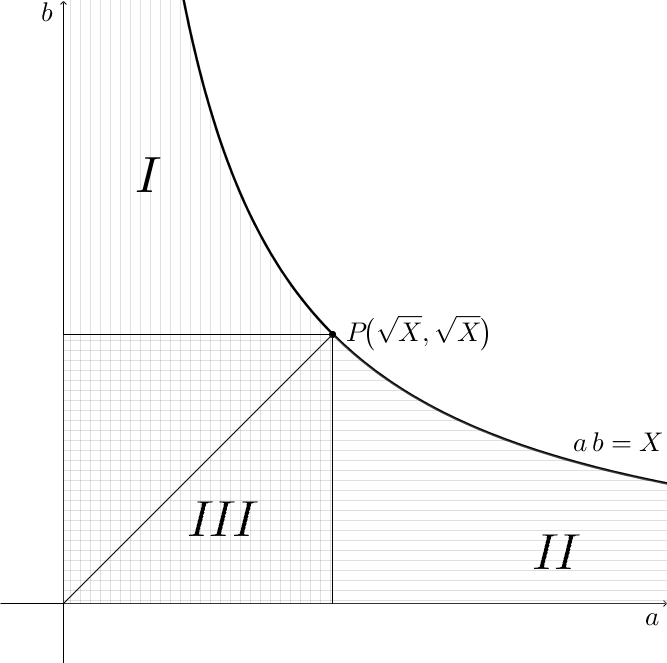
\includegraphics{fig1.png}
		\caption{La porzione di piano sottesa da \(a\,b=X\), suddivisa in \(3\) regioni.}
		\label{fig:2.7}
	\end{centering}
\end{figure}

\begin{oss}
	Un risultato molto più debole
	\[
		\sum_{n\le X} d(n)=X\ln X+O(X),
	\]
	può essere ottenuto più facilmente troncando il secondo termine significativo, infatti
	\[
		\begin{split}
			\sum_{n\le X}\sum_{d\mid n}1 & =\sum_{d\le X}\sum_{\substack{n\le X\\d\mid n}}1\\
			& =\sum_{d\le X}\left[\frac{X}{d}\right]\\
			& =\sum_{d\le X}\frac{X}{d}-\underbrace{\sum_{d\le X}\left\{\frac{X}{d}\right\}}_{\le X=O(X)}\\
			& =X\sum_{d\le X}\frac{1}{d}+O(X)\\
			& =X\left[\ln X+\g+O\left(\frac{1}{X}\right)\right]+O(X)\\
			& =X\ln X+\g X+O(1)+O(X)\graffito{i termini \(O(1)\) e \(\g X\) vengono inglobati da \(O(X)\)}\\
			& =X\ln X+O(X).
		\end{split}
	\]
\end{oss}

\begin{oss}
	Esiste una congettura, equivalente all'ipotesi di Riemann, che stima l'errore di
	\[
		\sum_{n\le X}d(n),
	\]
	come \(O\big(X^{1/4}\big)\).
\end{oss}

\begin{teor}{Stima superiore della funzione somma dei divisori}{2.9}
	Consideriamo la funzione somma dei divisori \(\s\), allora
	\[
		\s(n)\ll n\ln n.
	\]
\end{teor}

\begin{proof}
	Osserviamo che l'applicazione
	\[
		\mathcal{D}(n)\to\mathcal{D}(n),d\mapsto\frac{n}{d},
	\]
	è un involuzione, ovvero è un applicazione biunivoca che ha se stessa come inversa.
	Da cui
	\[
		\s(n)=\sum_{d\mid n}d=\sum_{d\mid n}\frac{n}{d}.
	\]
	Segue
	\[
		\begin{split}
			\s(n) & =\sum_{d\mid n}\frac{n}{d}\\
			& =n\sum_{d\mid n}\frac{1}{d} \le n\sum_{d\le n}\frac{1}{d}\\
			& =n\left[\ln n+\g+O\left(\frac{1}{b}\right)\right] \le 2n\ln n,
		\end{split}
	\]
	quando \(n\) è sufficientemente grande.
	Ovvero \(\s(n)\ll n\ln n\).
\end{proof}

\begin{teor}{Stima asintotica della funzione somma dei divisori}{2.10}
	Consideriamo la funzione somma dei divisori \(\s\), allora
	\[
		\sum_{n\le X}\s(n)=\frac{\p^2}{12}X^2+O(X\ln X).
	\]
\end{teor}

\begin{proof}
	Per definizione di \(\s\) avremo
	\[
		\begin{split}
			\sum_{n\le X}\s(n) & =\sum_{n\le X}\sum_{d\mid n}d = \sum_{n\le X}\sum_{d\mid n}\frac{n}{d}\graffito{vedi la dimostrazione del teorema precedente}\\
			& =\sum_{d\le X}\sum_{\substack{n\le X\\d\mid n}}\frac{d}{n} = \sum_{d\le X}\sum_{m\le \frac{X}{d}}m,
		\end{split}
	\]
	dove l'ultima uguaglianza è vera in quanto \(d\mid n\) implica \(n=m\,d\), inoltre \(n\le X\), da cui
	\[
		m=\frac{n}{d}\le \frac{X}{d}.
	\]
	Ricordiamo la ben nota formula per la somma dei primi \(N\) numeri interi
	\[
		\sum_{k=1}^N k=\frac{N(N+1)}{2},
	\]
	da cui
	\[
		\begin{split}
			\sum_{d\le X}\sum_{m\le\frac{X}{d}}m & =\sum_{d\le X}\frac{1}{2}\left[\frac{X}{d}\right]\left(\left[\frac{X}{d}\right]+1\right)\\
			& =\frac{1}{2}\sum_{d\le X}\left(\frac{X}{d}+O(1)\right)\left(\frac{X}{d}+O(1)\right)=\frac{1}{2}\sum_{d\le X}\left(\frac{X^2}{d^2}+O\left(\frac{X}{d}\right)\right)\\
			& =\frac{X^2}{2}\sum_{d\le X}\frac{1}{d^2}+O\underbrace{\left(X\sum_{d\le X}\frac{1}{d}\right)}_{\ll X\ln X}\graffito{per il teorema precedente}\\
			& =\frac{X^2}{2}\sum_{d=1}^{+\infty}\frac{1}{d^2}+O(X\ln X)-\frac{X^2}{2}\left(\sum_{d>X}\frac{1}{d^2}\right).
		\end{split}
	\]
	Ricordiamo il criterio del confronto integrale per serie:
	\[
		\int_1^X f(t)\,\dd t\ll \sum_{n=1}^X f(n) \ll \int_1^X f(t)\,\dd t,
	\]
	dove \(f\) è continua e \(f\ge 0\).
	Quindi
	\[
		\sum_{d\ge X}\frac{1}{d^2}\ll \int_X^{+\infty}\frac{\dd t}{t^2}=\frac{1}{X},
	\]
	ovvero
	\[
		\frac{X^2}{2}\left(\sum_{d\ge X}\frac{1}{d^2}\right)=O\left(X^2\frac{1}{X}\right)=O(X),
	\]
	infine, dal momento che il termine \(O(X)\) viene inglobato da \(O(X\ln X)\), avremo
	\[
		\begin{split}
			\sum_{n\le X}\s(n) & =\frac{X^2}{2}\sum_{d=1}^{+\infty}\frac{1}{d^2}+O(X\ln X)\\
			& =\frac{\p^2}{12}X^2+O(X\ln X).\qedhere
		\end{split}
	\]
\end{proof}
%%%%%%%%%%%%%%%%%%%%%%%%%%%%%%%%%%%%%%%%%
%
%LEZIONE 08/03/2016 - TERZA SETTIMANA (1)
%
%%%%%%%%%%%%%%%%%%%%%%%%%%%%%%%%%%%%%%%%%
%%%%%%%%%%%%%%%%%%%%%
%FUNZIONE DI MOEBIUS%
%%%%%%%%%%%%%%%%%%%%%
\section{Funzione di M\"oebius}

\begin{defn}{Funzione di M\"oebius}{funzioneMoebius}\index{Funzione!di M\"oebius}
	Si definisce \emph{funzione di M\"oebius} la seguente funzione aritmetica
	\[
		\m(n)=
		\begin{cases}
			1      & \text{se }n=1                            \\
			(-1)^s & \text{se }n=p_1\cdot\ldots\cdot p_s      \\
			0      & \text{se \(n\) ha un fattore quadratico}
		\end{cases}
	\]
\end{defn}

\begin{oss}
	Dire che \(n\) ha fattori moltiplicativi, significa affermare che esiste \(p\) primo tale che
	\[
		p^2 \mid n.
	\]
\end{oss}

\begin{teor}{\(\m\) è moltiplicativa}{2.11}
	La funzione \(\m\) di M\"oebius è moltiplicativa.
\end{teor}

\begin{proof}
	Siano \(n,m \in \N:(n,m)=1\), dobbiamo mostrare che \(\m(m\,n)=\m(m) \m(n)\).
	D'altronde se \(\m(m)\m(n)=0\) certamente esisterà un primo \(p\) tale che \(p^2\) divide \(n\) oppure \(m\), in entrambi i casi
	\[
		\ex p^2 \mid n\,m \implies \m(n\,m)=0.
	\]
	Se, invece, \(\m(n)\m(m) \neq 0\) avremo due possibilità
	\begin{itemize}
		\item \(n=1\) o \(m=1\), da cui segue banalmente la tesi;
		\item \(n \neq 1\) e \(m \neq 1\), quindi, per definizione di \(\m\)
		      \begin{gather*}
			      n = p_1 \cdot\ldots\cdot p_s,\\
			      m = q_1 \cdot\ldots\cdot q_r,
		      \end{gather*}
		      quindi \(\m(n) = (-1)^s\) e \(\m(m) = (-1)^r\).
		      Inoltre \(\m(n\,m) = (-1)^{r+s}\) in quanto \((n,m)=1\) implica che \(p_i \neq q_j,\,\fa i,j\).
	\end{itemize}
\end{proof}

\begin{oss}
	\(\m\) non è totalmente moltiplicativa, infatti
	\[
		1 = \m(2)\m(2) \neq \m(4) = 0.
	\]
\end{oss}

\begin{teor}{Trasformata di Dirichlet di \(\m\)}{2.12}
	La trasformate di Dirichlet di \(\m\) è
	\[
		\sum_{d\mid n}\m(d)=
		\begin{cases}
			1 & n=1     \\
			0 & n\neq 1
		\end{cases}
	\]
\end{teor}

\begin{proof}
	Ricordiamo che per il teorema \ref{th:2.1} la trasformata di Dirichlet di una funzione moltiplicativa è a sua volta moltiplicativa, quindi
	\[
		g(n)=\sum_{d\mid n}\m(d),
	\]
	è moltiplicativa in \(n\).
	Ora
	\[
		g(1)=\sum_{d\mid 1}\m(d)=\m(1)=1,
	\]
	inoltre, se \(\a \ge 1\),
	\[
		g(p^\a)=\sum_{d\mid p^\a}\m(d)=\sum_{\b=0}^\a \m(p^\b)=1-1=0.
	\]
	Infine, per la moltiplicatività di \(g\), avremo
	\[
		\begin{split}
			g(n) & =g \big( p_1^{\alpha_1}\cdot \ldots \cdot p_s^{\alpha_s} \big)\\
			& =g \big( p_1^{\a_1} \big) \cdot \ldots \cdot g \big( p_s^{\a_s} \big)\\
			& =0.\qedhere
		\end{split}
	\]
\end{proof}

\begin{teor}{Prima legge di inversione di M\"oebius}{2.13}
	Sia \(f\colon \N\to\C\) una funzione aritmetica.
	Sia \(g\colon \N\to\C\) la trasformata di Dirichlet di \(f\), allora
	\[
		g(n)=\sum_{d\mid n}f(d) \implies f(n)=\sum_{d\mid n}\mu(d) g\!\left( \frac{n}{d}\right).
	\]
\end{teor}

\begin{proof}
	Ricordiamo che esiste una corrispondenda biunivoca dell'inisieme dei divisori di \(n\) in se stesso tramite \(d\mapsto \frac{n}{d}\), per cui
	\[
		\begin{split}
			\sum_{d\mid n}\m(d) g\!\left( \frac{n}{d} \right) & =\sum_{d\mid n}\m \left( \frac{n}{d} \right) g(d)\\
			& =\sum_{d\mid n}\m \left( \frac{n}{d} \right) \sum_{e\mid d} f(e)\graffito{\(e\mid d,d\mid n\implies e\mid n\)}\\
			& =\sum_{e\mid n}f(e)\sum_{\substack{d\mid n\\e\mid d}}\m \left( \frac{n}{d} \right),
		\end{split}
	\]
	dove \(e,n\) sono fissati, inoltre \(n=d\, f,d=e\,k\), per cui
	\[
		f=\frac{n}{d}=\frac{n}{e\,k}\implies f\mid \frac{n}{e}.
	\]
	In conclusione
	\[
		\sum_{\substack{d\mid n\\e\mid d}}\m \left( \frac{n}{d} \right) =\sum_{f\mid \frac{n}{e}}\m(f)=
		\begin{cases}
			1 & e=n               \\
			0 & \text{altrimenti}
		\end{cases}
	\]
	ovvero
	\[
		\sum_{e\mid n}f(e)\sum_{\substack{d\mid n\\e\mid d}}\m \left( \frac{n}{d} \right) =f(n).
	\]
\end{proof}

\begin{ese}\label{es:z_f}
	Consideriamo la funzione \(\zeta\) di Riemann
	\[
		\zeta(s)=\sum_{n=1}^{+\infty}\frac{1}{n^s},s>1\graffito{in generale \(s\in\C\) con \(\Re(s)>1\)}
	\]
	e consideriamo
	\[
		F(s)=\sum_{n=1}^{+\infty}\frac{\m(n)}{n^s},
	\]
	dove \(\abs{\m(s)}\in\{0,1\}\), per cui \(F(s)\) converge totalmente per la convergenza di \(\zeta(s)\) quando \(s>1\).

	Facciamo il prodotto tra le due funzioni
	\[
		\sum_{n=1}^{+\infty}\frac{1}{n^s} \sum_{m=1}^{+\infty}\frac{\m(m)}{m^s} = \sum_{\substack{n\in\N\\m\in\N}}\frac{\m(m)}{(m\,n)^s} = \sum_{k=1}^{+\infty}\frac{a_k}{k^s},
	\]
	dove
	\[
		a_k=\sum_{\substack{n,m\in\N\\m\,n=k}}\m(m)=\sum_{m\mid k}\m(m)=
		\begin{cases}
			1 & k=1     \\
			0 & k\neq 1
		\end{cases}
	\]
	Ovvero
	\[
		\sum_{k=1}^{+\infty}\frac{a_k}{k^s}=1,
	\]
	cioè \(F\) è la funzione inversa di \(\zeta\), quindi
	\[
		\frac{1}{\z(s)}=\sum_{n=1}^{+\infty}\frac{\m(n)}{n^s}.
	\]
\end{ese}
%%%%%%%%%%%%%%%%%%%%%%%%%%%%%%%%%%%%%%%%%
%
%LEZIONE 10/03/2016 - TERZA SETTIMANA (2)
%
%%%%%%%%%%%%%%%%%%%%%%%%%%%%%%%%%%%%%%%%%
\begin{teor}{Seconda legge di inversione di M\"oebius}{teor.2.14}
	Siano \(g\colon\N\to\C\) e \(f\colon\N\to\C\) funzioni aritmetiche tali che
	\[
		f(n)=\sum_{d\mid n}\m(d) g\!\left( \frac{n}{d} \right) ,
	\]
	allora
	\[
		g(n)=\sum_{d\mid n}f(d).
	\]
\end{teor}

\begin{proof}
	La dimostrazione è analoga a quella del teorema \ref{th:2.13}, infatti
	\[
		\begin{split}
			\sum_{d\mid n}f(d) & = \sum_{d\mid n}\sum_{e\mid d}\m \left( \frac{d}{e} \right)g(e)\\
			& = \sum_{e\mid n}g(e)\sum_{d\mid \frac{n}{e}}\m \left( \frac{n}{e\,d} \right)\graffito{dalla corrispondenza biunivoca di \(\mathcal{D}(\frac{n}{d})\) in se stesso}\\
			& = \sum_{e\mid n}g(e) \left( \sum_{d\mid \frac{n}{e}}\m(d) \right)\\
			& = g(n).
		\end{split}
	\]
\end{proof}
%%%%%%%%%%%%%%%%%%%%
%FUNZIONE DI EULERO%
%%%%%%%%%%%%%%%%%%%%
\section{Funzione di Eulero}

\begin{defn}{Funzione di Eulero}{funzioneEulero}\index{Funzione!di Eulero}
	Si definisce funzione di Eulero
	\[
		\j(n)=\#\Set{x\in\N | x\le n,(x,n)=1}.
	\]
\end{defn}

\begin{oss}
	Analogamente \(\j\) si può definire come la cardinalità degli invertibili di \(\Z_n\), ovvero
	\[
		\j(n)=\#\mathcal{U}\left( \frac{\Z}{n\,\Z} \right).
	\]
\end{oss}

\begin{teor}{Trasformata di Dirichlet di \(\j\)}{2.15}
	La trasformata di Dirichlet di \(\j\) è
	\[
		\sum_{d\mid n}\j(d)=n.
	\]
\end{teor}

\begin{proof}
	Per ogni divisore \(d\) di \(n\) consideriamo
	\[
		\mathcal{D}_d=\Set{x\in\N | x\le n,(x,n)=d}\subseteq\Set{1,\ldots,n}.
	\]
	Osserviamo che se \(d\neq d'\) avremo \(\mathcal{D}_d\cap\mathcal{D}_{d'}=\emptyset\), per cui
	\[
		\bigsqcup_{d\mid n}\mathcal{D}_d=\Set{1,\ldots,n},
	\]
	ovvero
	\[
		n=\#\Set{1,\ldots,n}=\#\left( \bigsqcup_{d\mid n}\mathcal{D}_d \right)=\sum_{d\mid n}\big\lvert\mathcal{D}_d\big\rvert.
	\]
	Consideriamo ora
	\[
		\mathcal{D'}_d=\Set{x\in\N | 1\le x\le \frac{n}{d},\left( x,\frac{n}{d} \right)=1},
	\]
	quindi, per definizione, \(\big\lvert\mathcal{D'}_d\big\rvert=\j(\frac{n}{d})\).
	Esiste una corrispondenza biunivoca fra \(\mathcal{D}_d\) e \(\mathcal{D'}_d\) tramite
	\begin{gather*}
		x\mapsto \frac{x}{d}\\
		d\,y\mapsfrom y.
	\end{gather*}
	Per cui
	\[
		\begin{split}
			n & =\sum_{d\mid n}\big\lvert\mathcal{D}_d\big\rvert=\sum_{d\mid n}\big\lvert\mathcal{D'}_d\big\rvert\\
			& =\sum_{d\mid n}\j \left( \frac{n}{d} \right)=\sum_{d\mid n}\j(d).\qedhere
		\end{split}
	\]
\end{proof}

\begin{teor}{Inversione di M\"oebius applicata a \(\j\)}{2.16}
	La funzione \(\j\) di Eulero può essere riscritta nella forma
	\[
		\j(n)=\sum_{d\mid n}\m(d)\frac{n}{d}.
	\]
\end{teor}

\begin{proof}
	Segue banalmente dalla prima legge di inversione di M\"oebius (teorema \ref{th:2.13}).
	Infatti, dal teorema precedente sappiamo che
	\[
		\sum_{d\mid n}\j(d)=n,
	\]
	quindi conosciamo la trasformata di Dirichlet di \(\j\), applicando la legge di inversione otteniamo
	\[
		\j(n)=\sum_{d\mid n}\m(d)\frac{n}{d}.\qedhere
	\]
\end{proof}

\begin{teor}{\(\j\) è moltiplicativa}{2.17}
	La funzione \(\j\) di Eulero è moltiplicativa.
\end{teor}

\begin{proof}
	Dal teorema precedente sappiamo che
	\[
		\j(n)=\sum_{d\mid n}\m(d)\frac{n}{d},
	\]
	ora, la funzione \(\m\) di M\"oebius è moltiplicativa, pertanto lo sarà anche \(\m(d)/d\).
	Inoltre
	\[
		\sum_{d\mid n}\frac{\m(d)}{d},
	\]
	è moltiplicativa in quanto trasformata di Dirichlet di una funzione moltiplicativa.
	Quindi
	\[
		\j(n)=n\sum_{d\mid n}\frac{\m(d)}{d},
	\]
	è moltiplicativa.
\end{proof}

\begin{teor}{Scrittura alternativa di \(\j\)}{2.18}
	Supponiamo \(n>1\) e sia \(n=p_1^{\a_1}\cdot\ldots\cdot p_s^{\a_s}\), allora
	\[
		\j(n)=n\prod_{j=1}^s \left( 1- \frac{1}{p_s} \right).
	\]
\end{teor}

\begin{proof}
	Dal teorema \ref{th:2.16} sappiamo che
	\[
		\j(n)=n\sum_{d\mid n} \frac{\m(d)}{d},
	\]
	definiamo quindi la funzione
	\[
		h(n):=\sum_{d\mid n}\frac{\m(d)}{d}
	\]
	che per definizione è moltiplicativa.
	Quindi
	\[
		h(n)=\prod_{j=1}^s h\big(p_j^{\a_j}\big),
	\]
	dove
	\[
		h \big( p_s^{\a_j} \big)=1+\frac{\m(p_j)}{p_j}+\underbrace{\frac{\m(p_j^2)}{p_j^2}+\ldots}_{=0}=1- \frac{1}{p_j}.
	\]
	Per cui, sostituendo nell'equazione iniziale,
	\[
		\j(n)=n\,h(n)=n\prod_{j=1}^s \left( 1- \frac{1}{p_j} \right).\qedhere
	\]
\end{proof}

\begin{oss}
	L'ultima uguaglianza può essere ancora raffinata, infatti
	\[
		n\prod_{j=1}^s \left( 1- \frac{1}{p_j} \right) = \prod_{j=1}^s p_s^{\a_j}\prod_{j=1}^s \left( 1- \frac{1}{p_j} \right)=\prod_{j=1}^s \big( p_s^{\a_j}-p_j^{\a_{j-1}} \big).
	\]
\end{oss}

\begin{teor}{Disuguaglianza applicata a \(\j(n)\s(n)\)}{2.19}
	Vale la seguente disuguaglianza
	\[
		\frac{1}{2} < \frac{\j(n)\s(n)}{n^2} <1.
	\]
\end{teor}

\begin{proof}
	Preso \(n\in\N\), scriviamone la fattorizzazione \(n=p_1^{\a_1}\cdot\ldots\cdot p_s^{\a_s}\).
	Richiamando i teoremi \ref{pr:2.2} e \ref{th:2.18} avremo che
	\[
		\s(n)=\prod_{j=1}^s \frac{p_j^{\a_j+1}-1}{p_j-1}=\prod_{j=1}^s \frac{p_j^{\a_j+1} \big( 1-p_j^{-\a_j-1} \big)}{p_j(1-p_j^{-1})}=n\prod_{j=1}^s \frac{1-p_j^{-\a_j-1}}{1-p_j^{-1}},
	\]
	e
	\[
		\j(n)=n\prod_{j=1}^s \left( 1- \frac{1}{p_j} \right).
	\]
	Quindi
	\[
		\begin{split}
			\frac{\j(n)\s(n)}{n^2} & =\prod_{j=1}^s \left( 1- \frac{1}{p_j} \right)\prod_{j=1}^s \frac{1-p_j^{-\a_j-1}}{1-p_j^{-1}}\\
			& =\prod_{j=1}^s (1-p_j^{-1})\frac{1-p_j^{-\a_j-1}}{1-p_j^{-1}}\\
			& =\prod_{j=1}^s 1- \frac{1}{p_j^{\a_j+1}}<1.
		\end{split}
	\]
	Inoltre
	\[
		\begin{split}
			\prod_{j=1}^s \left( 1- \frac{1}{p_j^{a_j+1}} \right) & >\prod_{j=1}^s \left( 1- \frac{1}{p_j^2} \right)\\
			& >\prod_{m=2}^n \left( 1- \frac{1}{m^2} \right)\\
			& =\frac{n+1}{2n}>\frac{1}{2},
		\end{split}
	\]
	dove l'ultima uguaglianza si mostra facilmente per induzione.
\end{proof}

\begin{oss}
	La stima inferiore può essere migliorata, infatti
	\[
		\prod_{j=1}^s \left( 1- \frac{1}{p_j^{\a_j+1}} \right)>	\prod_p \left( 1- \frac{1}{p^2} \right)=\frac{1}{\z(2)} =\frac{6}{\p^2}.
	\]
\end{oss}

\begin{teor}{Stima inferiore di \(\j\)}{2.20}
	Vale la seguente stima
	\[
		\j(n) \gg \frac{n}{\ln n},\text{ per }n\to +\infty.
	\]
\end{teor}

\begin{proof}
	Dal teorema \ref{th:2.9} sappiamo che
	\[
		\s(n) \ll n\ln n \iff \frac{1}{\s(n)} \gg \frac{1}{n\ln n},
	\]
	ora, per il teorema precedente
	\[
		\j(n)> \frac{n^2}{2\s(n)} \iff \j(n) \gg \frac{n}{\ln n}.\qedhere
	\]
\end{proof}

\begin{oss}
	Si può dimostrare che in particolare vale il seguente
	\[
		\j(n)> \frac{n}{e^\g \ln(\ln n)+\frac{3}{\ln(\ln n)}},
	\]
	ovvero
	\[
		\j(n) \gg \frac{n}{\ln(\ln n)}.
	\]
	Inoltre \(\j(n)\le n-1\) quando \(n\neq 1\), quindi, in conclusione,
	\[
		\frac{n}{\ln(\ln n)}\ll \j(n) \le n-1.
	\]
\end{oss}

\begin{ese}
	Sappiamo che
	\[
		\z(s)=\sum_{n=1}^{+\infty} \frac{1}{n^s}\qquad\text{e}\qquad \frac{1}{\z(s)}=\sum_{n=1}^{+\infty} \frac{\m(n)}{n^s},
	\]
	allora
	\[
		\frac{\z(s-1)}{\z(s)}=\sum_{n=1}^{+\infty}\frac{\j(n)}{n^s},\Re(s)>2.
	\]
\end{ese}

\begin{oss}
	Si può dimostrare che anche
	\[
		\sum_{n=1}^{+\infty}\frac{d(n)}{n^s},
	\]
	può essere scritto in funzione di \(\z(s)\).
\end{oss}

\begin{teor}{Stima asintotica di \(\j\)}{2.21}
	Vale la seguente stima
	\[
		\sum_{n\le X}\j(n)=\frac{3}{\p^2}X^2+O(X\ln X).
	\]
\end{teor}

\begin{proof}
	Applicando il teorema di inversione (\ref{th:2.13}), otteniamo
	\[
		\begin{split}
			\sum_{n\le X}\j(n) & =\sum_{n\le X}\sum_{d\mid n}\frac{n}{d}\m(d)\\
			& =\sum_{d\le X}\frac{\m(d)}{d}\sum_{\substack{n\le X\\d\mid n}}n\\
			& =\sum_{d\le X}\frac{\m(d)}{d}\sum_{m\le \frac{X}{d}}m\,d.
		\end{split}
	\]
	Ora
	\[
		\sum_{r\le T}r=\frac{1}{2}[T]\big( [T]+1 \big)=\frac{1}{2}T^2+O(T).
	\]
	Quindi, sostituendo nell'equazione iniziale, otteniamo
	\[
		\begin{split}
			\sum_{d\le X}\m(d)\sum_{m\le \frac{X}{d}}m & =\sum_{d\le X}\m(d)\left[ \frac{1}{2}\frac{X^2}{d^2}+O \left( \frac{X}{d} \right) \right]\\
			& =\frac{1}{2}\left( \sum_{d\le X} \frac{\m(d)}{d^2} \right)X^2+O \left( \sum_{d\le X} \frac{X}{d} \right)\graffito{ho stimato \(\m(d)=1\)}\\
			& =\frac{1}{2}\left[ \frac{1}{\z(2)}+O \left( \frac{1}{X} \right) \right] X^2+O(X\ln X)\\
			& =\frac{1}{2\z(2)}X^2+O(X\ln X)=\frac{3}{\p^2}X^2+O(X\ln X).
		\end{split}
	\]
	dove
	\[
		\sum_{d\le X} \frac{\m(d)}{d^2}=\frac{1}{\z(2)}+O \left( \frac{1}{X} \right)\qquad\text{e}\qquad O \left( \sum_{d\le X} \frac{X}{d} \right)=O(X\ln X),
	\]
	valgono rispettivamente per l'esercizio \ref{ex:1.6} e per il l'osservazione alla stima della serie armonica (teorema \ref{th:2.8}).
\end{proof}

\begin{oss}
	Esiste una congettura, equivalente all'ipotesi di Riemann, per cui
	\[
		\sum_{n\le X}\j(n)=\frac{3}{\p^2}X^2+O \big( X^{\frac{1}{2}+\e} \big).
	\]
\end{oss}
%%%%%%%%%%%%%%%%%%%%%%%%%%%%%%%%%%%%%%%
%PRODOTTO DI CONVOLUZIONE DI DIRICHLET%
%%%%%%%%%%%%%%%%%%%%%%%%%%%%%%%%%%%%%%%
\section{Prodotto di convoluzione di Dirichlet}

\begin{defn}{Prodotto di convoluzione}{prodottoConvoluzione}\index{Prodotto di convoluzione}
	Siano \(f,g\colon\N\to\C\) due funzioni aritmetiche.
	Si definisce convoluzione (di Dirichlet) di \(f,g\) la seguente funzione
	\[
		\big( f*g \big)(n)=\sum_{d\mid n}f(d) g\!\left( \frac{n}{d} \right).
	\]
\end{defn}

\begin{oss}
	Le seguenti sono definizioni equivalenti
	\[
		\begin{split}
			\big( f*g \big)(n) & =\sum_{d\mid n}f\!\left( \frac{n}{d} \right)g(d)\\
			& =\sum_{\substack{a,b\in\N\\a\,b=n}}f(a)g(b).
		\end{split}
	\]
\end{oss}

\begin{ese}
	Se consideriamo la funzione unitaria \(u(n)=1\), allora \(u*f\) è la trasformata di Dirichlet di \(f\).
	Inoltre, per le leggi di inversioni
	\[
		u*f=g \iff f=\m*g.
	\]
\end{ese}

\begin{oss}
	In particolare avremo
	\[
		u * \d = u \iff \d = \m * u,
	\]
	ovvero \(\m\) è invertibile e \(\m^{-1}=u\).
\end{oss}

\begin{prop}{Funzioni aritmetiche costituiscono un monoide commutativo}{convoluzioneMonoide}
	Sia \(\mathcal{A}=\Set{f\colon\N\to \C}\).
	Allora
	\[
		(A,*),
	\]
	costituisce un monoide commutativo.
\end{prop}

\begin{proof}
	La dimostrazione è una semplice verifica:
	\begin{itemize}
		\item \(\big( f*g \big)*h=f*\big( g*h \big)\), in quanto
		      \[
			      \big( f*g \big)*h=\sum_{\substack{a,b,c\in\N\\a\,b\,c=n}}f(a)g(b)h(c);
		      \]
		\item \(f*g=g*f\) segue dalla definizione;
		\item \(\ex\d\in\mathcal{A}:f*\d=\d*f=f\) con
		      \[
			      \d(n) =
			      \begin{cases}
				      1 & n =1              \\
				      0 & \text{altrimenti}
			      \end{cases}
		      \]
	\end{itemize}
\end{proof}
%%%%%%%%%%%%%%%%%%%%%%%%%%%%%%%%%%%%%%%%%
%
%LEZIONE 11/03/2016 - TERZA SETTIMANA (3)
%
%%%%%%%%%%%%%%%%%%%%%%%%%%%%%%%%%%%%%%%%%
\begin{ese}
	Sia \(f \in \mathcal{A}\), possiamo associare ad \(f\) una serie
	\[
		\z_f(s)=\sum_{n\in\N} \frac{f(n)}{n^s},
	\]
	con \(s\) sufficientemente grande.
	Se ora consideriamo la funzione unitaria \(u\) e l'identità \(\d\), avremo
	\begin{gather*}
		\z_u(s)=\sum_{n\in\N} \frac{u(n)}{n^s} = \sum_{n\in\N} \frac{1}{n^s} = \z(s);\\
		\z_\d(s)=\sum_{n\in\N} \frac{\d(n)}{n^s} = 1.
	\end{gather*}
	Ora, se esistesse \(\a\in\R\) tale che \(f(n)=O(n^\a)\), si avrebbe \(\z_f(s) < +\infty\) per \(\Re(s)>\a+1\), infatti
	\[
		\abs{\z_f(s)} \le \sum_{n\in\N} \frac{\abs{f(n)}}{n^s} \ll \sum_{n\in\N} \frac{1}{n^{s-\a}} < +\infty,
	\]
	per \(s>\a+1\).
\end{ese}

\begin{lem}\label{lem:convz_f}
	Siano \(f,g\in \mathcal{A}\), allora
	\[
		\z_f(s) \z_g(s) = \z_{f*g}(s),
	\]
	per \(s\) sufficientemente grande.
\end{lem}

\begin{proof}
	Andremo a sfruttare la definizione equivalente di convoluzione, infatti
	\[
		\begin{split}
			\z_f(s) \z_g(s) & =\sum_{n\in\N} \frac{f(n)}{n^s} \sum_{m\in\N} \frac{g(m)}{m^s}\\
			& =\sum_{n,m\in\N} \frac{f(n)g(m)}{(n\,m)^s}\graffito{raggruppando le coppie con lo stesso prodotto}\\
			& =\sum_{k\in\N} \frac{1}{k^s} \sum_{\substack{n,m\in\N\\n\,m=k}} f(n)g(m)\\
			& =\sum_{k\in\N} \frac{\big(f*g\big)(k)}{k^s}\\
			& =\z_{f*g}(s).\qedhere
		\end{split}
	\]
\end{proof}

\begin{oss}
	Notiamo che possiamo scrivere la funzione somma dei divisori \(d(n)\) come la convoluzione della funzione unitaria \(u\) in se stessa, infatti
	\[
		\big( u*u \big)(n) = \sum_{d\mid n}u(d) u\!\left( \frac{n}{d} \right)=\sum_{d\mid n} 1 = d(n),
	\]
	quindi, per il lemma precedente
	\[
		\z_d(s)=\z_{u*u}(s)=\z_u(s) \z_u(s)=\big(\z_u(s)\big)^2=\big(\z(s)\big)^2.
	\]
\end{oss}

\begin{teor}{Invertibilità rispetto alla convoluzione}{2.22}
	Sia \(f\in\mathcal{A}\), allora
	\[
		f \in \mathcal{U}(\mathcal{A}) \iff f(1) \neq 0.
	\]
\end{teor}

\begin{proof}
	\graffito{\(\Rightarrow)\)}Se \(f\in\mathcal{U}(\mathcal{A})\), esiste \(g\in\mathcal{A}\) tale che
	\[
		f*g=\d.
	\]
	In particolare avremo \(\big(f*g\big)(1)=\d(1)=1\), ma
	\[
		\left( f*g \right)(1) = \sum_{\substack{a,b\in\N\\a\,b=1}}f(a) g(b)=f(1) g(1) = 1,
	\]
	quindi, necessariamente, \(f(1)\neq 0\).

	\graffito{\(\Leftarrow)\)}Costruiamo l'inversa \(g\) con un metodo induttivo. Definiamo \(g(1)\) come
	\[
		g(1):= \frac{1}{f(1)}.
	\]
	Procediamo con \(g(2)\), vogliamo che
	\[
		\big( f*g \big)(2) = \d(2) = 0,
	\]
	per cui
	\[
		\begin{split}
			0 = \big( f*g \big)(2) & = \sum_{\substack{a,b\in\N\\a\,b=2}}f(a)g(b)\\
			& = f(1)g(2) + f(2)g(1),
		\end{split}
	\]
	ovvero
	\[
		g(2) = -\frac{f(2)g(1)}{f(1)}.
	\]
	Generalizzando per \(n\neq 1\) avremo \(\big( f*g \big)(n)=\d(n)=0\), da cui
	\[
		\begin{split}
			0 = \big( f*g \big)(n) & = \sum_{d\mid n} f(d) g\!\left( \frac{n}{d} \right)\\
			& = f(1)g(n)+\sum_{\substack{d\mid n\\d\neq 1}} f(d) g\!\left( \frac{n}{d} \right),
		\end{split}
	\]
	ovvero
	\[
		g(n) = - \frac{1}{f(1)}\sum_{\substack{d\mid n\\d\neq 1}}f(d) g\!\left( \frac{n}{d} \right).
	\]
	Quindi avendo definito
	\[
		g(n) = 	\begin{cases}
			\displaystyle\frac{1}{f(1)} & n=1                    \\
			\displaystyle- \frac{1}{f(1)}\sum_{\substack{d\mid n \\d\neq 1}}f(d) g\!\left( \frac{n}{d} \right) & n\neq 1
		\end{cases}
	\]
	avremo che \(g\) è l'inversa di \(f\).
\end{proof}

\begin{oss}
	Quindi l'insieme
	\[
		\mathcal{A'}=\Set{f\in \mathcal{A} | f(1)\neq 0},
	\]
	è un gruppo abeliano rispetto alla composizione.
\end{oss}

\begin{defn}{Insieme delle funzioni moltiplicative}{insiemeMoltiplicative}
	Analogamente al caso delle funzioni funzioni aritmetiche, definiamo
	\[
		\mathcal{M} = \Set{f\colon\N\to\C | f\text{ moltiplicativa}},
	\]
	come l'insieme delle funzioni moltiplicative.
\end{defn}

\begin{teor}{\(\mathcal{M}\) è chiuso rispetto alla convoluzione}{2.24}
	Consideriamo l'insieme delle funzioni moltiplicative \(\mathcal{M}^*\) privo della funzione identicamente nulla.
	Allora \(\mathcal{M}^*\) è chiuso rispetto alla convoluzione.
\end{teor}

\begin{proof}
	Siano \(f,g\in\mathcal{M}^*\) e siano \(n,m\in\N\) tali che \((n,m)=1\), dobbiamo mostrare che
	\[
		\big( f*g \big)(m\,n) = \big( f*g \big)(m) \big( f*g \big)(n).
	\]
	Ora
	\[
		\begin{split}
			\big( f*g \big)(m\,n) & = \sum_{d\mid m\,n}f(d) g\!\left( \frac{m\,n}{d} \right)\graffito{ricordiamo che da \((n,m)=1\) si deduce una corrispondenza biunivoca tra \(\mathcal{D}(n\,m)\) e \(\mathcal{n}\times\mathcal{m}\)}\\
			& = \sum_{\substack{d_1\mid m\\d_2\mid n}} f(d_1 d_2) g\!\left( \frac{m}{d_1} \frac{n}{d_2} \right)\\
			& = \sum_{\substack{d_1\mid m\\d_2\mid n}} f(d_1) f(d_2) g\!\left( \frac{m}{d_1} \right) g\!\left( \frac{n}{d_2} \right)\\
			& = \left[ \sum_{d_1\mid m} f(d_1) g\!\left( \frac{m}{d_1} \right) \right] \left[ \sum_{d_2\mid n} f(d_2) g\!\left( \frac{n}{d_2} \right) \right]\\
			& = \left( f*g \right)(m) \left( f*g \right)(n).\qedhere
		\end{split}
	\]
\end{proof}
%%%%%%%%%%%
%APPENDICE%
%%%%%%%%%%%
\section{Appendice}

\begin{defn}{Numero privo di fattori quadratici}{numSFQ}
	\(n\in\N\) si dice privo di \emph{fattori quadratici} se la fattorizzazione in primi di \(n\) è costituita da primi a due a due distinti, ovvero
	\[
		n = p_1^ \cdot\ldots\cdot p_s,\text{ con }p_1 < \ldots < p_s.
	\]
\end{defn}

\begin{oss}
	Analogamente un numero \(n\in \N\) si definisce privo di fattori quadratici se \(p^2 \nmid n\) per ogni \(p\) primo.
\end{oss}

\begin{defn}{Funzione caratteristica dei numeri privi di fattori quadratici}{funzCarSFQ}
	Definiamo la \emph{funzione caratteristica} dei numeri privi di fattori quadratici come
	\[
		\m_2(n) =	\begin{cases}
			1 & \text{se \(n\) è privo di fattori quadratici} \\
			0 & altrimenti
		\end{cases}
	\]
\end{defn}

\begin{oss}
	Dalla definizione segue che
	\[
		\m_2(n) = \abs{\m(n)},
	\]
	dove \(\m\) è la funzione di M\"oebius.
	Da cui segue, per la moltiplicatività di \(\m\), che \(\m_2\) è moltiplicativa.
\end{oss}

\begin{prop}{Scrittura alternativa di \(\m_2\)}{scritturaAltSFQ}
	Consideriamo la funzione \(\m_2\), allora
	\[
		\m_2(n) = \sum_{d^2\mid n} \m(d).
	\]
\end{prop}

\begin{proof}
	Se \(n=1\)
	\[
		\sum_{d^2\mid 1}\m(d) = \m(1) = 1 = \m_2(1).
	\]
	Se \(n=p^\a\)
	\[
		\sum_{d^2\mid p^\a}\m(d) = 	\begin{cases}
			1 & \a = 1   \\
			0 & \a \ge 2
		\end{cases}
		= \m_2(p^\a).
	\]
	Infine, se \(n=p_1^{\a_1} \cdot\ldots\cdot p_s^{\a_s} \neq 1\), per la moltiplicatività di \(\m\) e di \(\m_2\) avremo
	\[
		\begin{split}
			\sum_{d^2\mid n}\m(n) & = \sum_{d^2\mid n}\m(p_1^{\a_1}) \cdot\ldots\cdot \m(p_s^{\a_s})\\
			& = \sum_{d_1^2\mid p_1^{\a_1}} \m(p_1^{\a_1}) \cdot\ldots\cdot \sum_{d_s^2\mid p_s^{\a_s}}\m(p_s^{\a_s})\\
			& = \m(p_1^{\a_1}) \cdot\ldots\cdot \m(p_s^{\a_s})\\
			& = \m(n).\qedhere
		\end{split}
	\]
\end{proof}

\begin{oss}
	Se definiamo la seguente funzione
	\[
		\c_2(k) = 	\begin{cases}
			1 & \text{se \(k\) è un quadrato} \\
			0 & \text{altrimenti}
		\end{cases}
	\]
	allora avremo
	\[
		\m_2(n) = \sum_{d\mid n} \c_2(d)\m(d).
	\]
\end{oss}

\begin{teor}{Stima della cardinalità di numeri privi di fattori quadratici}{cardSFQ}
	Vale la seguente stima
	\[
		\sum_{n\le X} \m_2(n) = \frac{6}{\p^2}X + O\big(\sqrt{X}\big).
	\]
\end{teor}

\begin{proof}
	Applicando la proposizione precedente avremo
	\[
		\begin{split}
			\sum_{n\le X} \m_2(n) & = \sum_{n\le X}\sum_{\substack{d\in\N\\d^2\mid n}} \m(d)\\
			& = \sum_{d\le \sqrt{X}} \m(d) \sum_{\substack{n\le X\\d^2\mid n}}1\graffito{per la proposizione \ref{pr:parteIntera9} sulla parte intera}\\
			& = \sum_{d\le \sqrt{X}} \m(d) \left[ \frac{X}{d^2} \right] = \sum_{d\le \sqrt{X}} \frac{\m(d)}{d^2} \big( X+O(1) \big)\\
			& = X \sum_{d\le \sqrt{X}} \frac{\m(d)}{d^2} + O \left( \sum_{d\le \sqrt{X}} \frac{\m(d)}{d^2} \right) \le X \sum_{d\le \sqrt{X}} \frac{\m(d)}{d^2} + O\big(\sqrt{X}\big)\graffito{ho stimato \(\frac{\m(d)}{d^2}\le 1\)}\\
			& = X \left( \frac{1}{\z(2)} + O \left( \frac{1}{\sqrt{X}} \right) \right) + O\big(\sqrt{X}\big)\\
			& = \frac{6}{\p^2}X + O\big(\sqrt{X}\big).
		\end{split}
	\]
	dove
	\[
		\sum_{d\le \sqrt{X}} \frac{\m(d)}{d^2} = \frac{1}{\z(2)} + O \left( \frac{1}{\sqrt{X}} \right),
	\]
	per l'esercizio \ref{ex:1.6}.
\end{proof}

\begin{oss}
	Quindi circa il \(60\%\) dei numeri è senza fattori quadratici.
\end{oss}
%!TEX root = ../main.tex
%%%%%%%%%%%%%%%%%%%%%%%%%%%%%%%%%%%%%%%%%
%
%LEZIONE 11/03/2016 - TERZA SETTIMANA (3)
%
%%%%%%%%%%%%%%%%%%%%%%%%%%%%%%%%%%%%%%%%%
\chapter{Congruenze}

\section{Introduzione}

\begin{defn}{Congruenza modulo \(n\)}{congruenza}\index{Congruenza}
	Presi \(a,b\in\Z\) e \(n\in\N\), diremo che \(a\) è congruo a \(b\) in modulo \(n\) se e soltanto se
	\[
		n \mid a-b.
	\]
\end{defn}

\begin{notz}
	Si scrive \(a\equiv b \pmod{n}\).
\end{notz}

\begin{oss}
	Se facciamo la divisione euclidea fra \(a\) ed \(n\) otteniamo
	\[
		a = n\,q + r,\text{ con }0\le r < n,
	\]
	ovvero \(a\equiv r \pmod{n}\).
\end{oss}

\begin{teor}{Caratterizzazione della congruenza}{3.1}
	Presi \(a,b\in\Z\) diremo che \(a\equiv b \pmod{n}\) se e soltanto se \(a\) e \(b\), divisi per \(n\), hanno lo stesso resto.
\end{teor}

\begin{proof}
	\graffito{\(\Leftarrow)\)}Supponiamo che
	\[
		a = n\,q_1 + r \qquad\text{e}\qquad b = n\,q_2 + r,
	\]
	sottraendo membro a membro avremo
	\[
		a-b = n(q_1 - q_2),
	\]
	ovvero \(n\mid a-b\), quindi, per definizione, \(a\equiv b \pmod{n}\).

	\graffito{\(\Rightarrow)\)}Supponiamo che \(n\mid a-b\), ovvero
	\[
		n\,q = a-b \iff a = n\,q + b,
	\]
	se effettuiamo la divisione euclidea fra \(a\) ed \(n\), avremo
	\[
		a = n\,q' + r,\text{ con }0\le r < n
	\]
	quindi, uguagliando le espressioni, otteniamo
	\[
		n\,q+b = n\,q'+r \iff b = n(q'-q) + r,
	\]
	dove \(0\le r < n\), da cui, per l'unicità dei resti, si ha la tesi.
\end{proof}

\begin{pr}\label{th:3.2}
	Siano \(a_1,a_2,b_1,b_2\in\Z\) e sia \(n\in\N\) tali che
	\[
		a_1\equiv b_1 \pmod{n}\qquad\text{e}\qquad a_2\equiv b_2 \pmod{n},
	\]
	allora
	\begin{itemize}
		\item \(a_1+a_2\equiv b_1+b_2 \pmod{n}\);
		\item \(a_1 a_2\equiv b_1 b_2 \pmod{n}\).
	\end{itemize}
\end{pr}

\begin{pr}\label{th:3.3}
	Siano \(a,b,c\in\Z\) e sia \(n\in\N\) con \(c\neq 0\), allora
	\begin{itemize}
		\item \(a\,c\equiv b\,c \pmod{n} \implies a\equiv b \pmod{n/(n,c)}\);
		\item \((n,c)=1 \implies a\equiv b \pmod{n}\).
	\end{itemize}
\end{pr}
%%%%%%%%%%%%%%%%%%%%
%SISTEMI DI RESIDUI%
%%%%%%%%%%%%%%%%%%%%
\section{Sistemi di residui}

\begin{defn}{Residuo modulo \(n\)}{residuo}\index{Residuo}
	Preso \(a\in\Z\), diremo che il resto di \(a\) diviso \(n\) è il \emph{residuo} di \(a\) modulo \(n\).
\end{defn}

\begin{defn}{Insieme completo di residui modulo \(n\)}{ICR}\index{Insieme completo di residui}
	Un insieme \(S\subseteq\Z\) si definisce \emph{insieme completo di residui modulo \(m\)} se, per ogni intero \(z\in\Z\), esiste un unico \(s\in S\) tale che
	\[
		z\equiv s \pmod{m}.
	\]
\end{defn}

\begin{notz}
	Spesso indicheremo un sistema completo di residui modulo \(m\) con la sigla ICR(\(m\)).
\end{notz}

\begin{pr*}
	Dato \(m\in\N\), allora \(S\subseteq \Z\) è un ICR(\(m\)) se e soltanto se
	\begin{itemize}
		\item \(\abs{S} = m\);
		\item \(\fa x,y \in S, x\neq y \implies x \not\equiv y \pmod{m}\).
	\end{itemize}
\end{pr*}

\begin{ese}
	Preso \(m\in\N\) l'insieme completo di residui canonico di \(m\) è
	\[
		S=\Set{0,1,\ldots,m-1}.
	\]
\end{ese}

\begin{ese}
	Analogamente sono sistemi completi di residui
	\begin{itemize}
		\item \(S=\Set{1,2,\ldots,m}\);
		\item se \(m\) è pari \(S=\Set{-m/2,\ldots,-1,0,1,\ldots,m/2-1}\).
	\end{itemize}
\end{ese}

\begin{teor}{Dilatazione di un ICR}{3.4}
	Sia \(S\) un insieme completo di residui modulo \(m\) e sia \(k\in\Z\) tale che \((k,m)=1\).
	Allora l'insieme
	\[
		k\,S = \Set{k\,x | x \in S},
	\]
	è ancora un insieme completo di residui modulo \(m\).
\end{teor}

\begin{proof}
	Basta dimostrare che vale la caratterizzazione:
	\begin{itemize}
		\item \(\abs{k\,S} = m\) segue banalmente da dalla definizione di \(k\,S\) e da \(\abs{S} = m\).
		\item Siano \(k\,x_1,k\,x_2\in k\,S\) distinti modulo \(m\).
		      Se per assurdo \(k\,x_1 \equiv k\,x_2 \pmod{m}\), si avrebbe
		      \[
			      x_1 \equiv x_2 \pmod{\frac{m}{(k,m)}} \iff x_1 \equiv x_2 \pmod{m},
		      \]
		      in quanto \((k,m) = 1\) per ipotesi.
		      Ma ciò è ovviamente assurdo in quanto \(x_1,x_2\) sono elementi distinti di un ICR(\(m\)).
	\end{itemize}
\end{proof}

\begin{defn}{Insieme completo di residui invertibili}{IRR}
	Sia \(S\) un insieme completo di residui modulo \(m\), si definisce \emph{insieme completo di residui invertibili modulo \(m\)}, l'insieme
	\[
		S^* = \Set{s\in S | (s,m) = 1}.
	\]
\end{defn}

\begin{notz}
	Spesso indicheremo un sistema completo di residui invertibili modulo \(m\) con la sigla IRR(\(m\)).
\end{notz}

\begin{pr*}
	Dato \(m\in\N\), allora \(S^*\subseteq \Z\) è un IRR(\(m\)) se e soltanto se
	\begin{itemize}
		\item \(\abs{S^*} = \j(m)\);
		\item \((a,m) = 1,\,\fa a \in S^*\);
		\item \(\fa x,y \in S^*, x\neq y \implies x\not\equiv y \pmod{m}\).
	\end{itemize}
\end{pr*}
%%%%%%%%%%%%%%%%%%%%%%%%%%%%%%%%%%%%%%%%%%
%
%LEZIONE 15/03/2016 - QUARTA SETTIMANA (1)
%
%%%%%%%%%%%%%%%%%%%%%%%%%%%%%%%%%%%%%%%%%%
\begin{teor}{Dilatazione di un ICR}{3.4'}
	Sia \(S^*\) un insieme completo di residui invertibili modulo \(m\) e sia \(k\in\Z\) tale che \((k,m)=1\).
	Allora l'insieme
	\[
		k\,S^* = \Set{k\,x | x \in S^*},
	\]
	è ancora un insieme completo di residui completo modulo \(m\).
\end{teor}

\begin{proof}
	La dimostrazione è analoga a quella sugli insiemi completi (teorema \ref{th:3.4}), resta solo da mostrare che
	\[
		k\,x \in k\,S^* \implies (k\,x,m) = 1.
	\]
	Ma \(x\in S^*\) implica \((x,m) = 1\), mentre \((k,m) = 1\) per ipotesi, per cui
	\[
		(x\,k,m) = 1.\qedhere
	\]
\end{proof}

\begin{oss}
	Se \(S\) è ICR(\(m\)) allora \(S+a\) è ancora ICR(\(m\)).
	Ma questo, in generale, non vale per gli IRR.
\end{oss}

\begin{teor}{Combinazione lineare di ICR}{3.5}
	Siano \(a,b\in\N\) tali che \((a,b)=1\) e supponiamo che \(S_a\) sia un ICR(\(a\)) e che \(S_b\) sia un ICR(\(b\)), allora
	\[
		b\,S_a + a\,S_b,
	\]
	è un ICR(\(a\,b\)).
\end{teor}

\begin{proof}
	Mostriamo che vale la caratterizzazione:
	\begin{itemize}
		\item Vogliamo mostrare che \(\#(b\,S_a + a\,S_b) = a\,b\).
		      Ora
		      \[
			      b\,S_a + a\,S_b = \Set{b\,x + a\,y | x\in S_a, y\in S_b},
		      \]
		      dove \(\abs{S_a} = a\) e \(\abs{S_b} = b\).
		      Quindi ci basta verificare che se \((x_1,y_1) \neq (x_2,y_2)\) allora \(x_1 b + y_1 a \not\equiv x_2 b + y_2 a\).
		      Supponiamo per assurdo che \(x_1 b + y_1 a \equiv x_2 b + y_2 a\), allora
		      \[
			      \begin{split}
				      b \mid a(y_1-y_2) & \implies b \mid y_1-y_2 \graffito{dal momento che \((a,b) = 1\)}\\
				      & \implies y_1\equiv y_2 \pmod{b} \implies y_1 = y_2,
			      \end{split}
		      \]
		      per la caratterizzazione degli ICR.
		      Analogamente segue che \(x_1 = x_2\).
		      Ma ciò è assurdo per la scelta di \(x_1,x_2,y_1,y_2\).
		\item Il ragionamento precedente è valido anche per mostrare che
		      \[
			      x_1 b + y_1 a \not\equiv x_2 b + y_2 a \pmod{a\,b}.\qedhere
		      \]
	\end{itemize}
\end{proof}

\begin{cor}
	Se \(S_a^*\) è un IRR(\(a\)) e \(S_b^*\) è un IRR(\(b\)), allora
	\[
		b\,S_a^* + a\,S_b^*,
	\]
	è un IRR(a\,b).
\end{cor}

\begin{proof}
	La dimostrazione segue da quella precedente, eccetto per la verifica che
	\[
		(b\,x+a\,y,a\,b) = 1.
	\]
	Osserviamo che \((b\,x+a\,y,a)=(b\,x,a) = (x,a)\) in quanto \((a,b) = 1\), e che \((x,a) = 1\) poichè \(x\in S\).
	Analogamente si mostra che \((b\,x+a\,y,b) = (a\,y,b) = (y,b) =1\).
	Per cui
	\[
		(a\,x+b\,y,a\,b) = 1.\qedhere
	\]
\end{proof}
%%%%%%%%%%%%%%%%%%%%%%%%%%%%%%%
%TEOREMI DI EULERO E DI FERMAT%
%%%%%%%%%%%%%%%%%%%%%%%%%%%%%%%
\section{Teoremi di Eulero e di Fermat}

\begin{teor}{di Eulero-Fermat}{3.6}\index{Teorema!di Eulero-Fermat}
	Preso \(m\in\N\), sia \(a\in\Z\) tale che \((a,m) = 1\), allora
	\[
		a^{\j(m)} \equiv 1 \pmod{m}.
	\]
\end{teor}

\begin{proof}
	Sia \(S^*\) un qualsiasi IRR(\(m\)), allora sappiamo che anche \(a\,S^*\) è un IRR(\(m\)).
	Ora
	\[
		\prod_{j\in S^*} j \equiv \prod_{a\,j \in S^*} a\,j \pmod{m}.
	\]
	Inoltre, siccome \(\abs{S^*} = \j(m)\), avremo
	\[
		\prod_{j\in S^*}j \equiv a^{\j(m)} \prod_{j\in S^*} j \pmod{m},
	\]
	dove \((m,j) = 1\) comunque prendo \(j\in S^*\), per cui
	\[
		\left( m, \prod_{j\in S^*} j \right)=1,
	\]
	quindi
	\[
		1 \equiv a^{\j(m)} \pmod{m}\qedhere
	\]
\end{proof}

\begin{teor}{Piccolo teorema di Fermat}{3.7}\index{Teorema!di Fermat (piccolo)}
	Sia \(p\) primo e sia \(a\in\Z\) tale che \(p\nmid a\), allora
	\[
		a^{p-1} \equiv 1 \pmod{p}
	\]
\end{teor}

\begin{proof}
	Dal momento che \(p\) è primo e che non divide \(a\), avremo necessariamente
	\[
		(a,p) = 1.
	\]
	Quindi, applicando il teorema precedente, avremo
	\[
		a^{\j(p)} \equiv 1 \pmod{p},
	\]
	ovvero, ricordando che \(p\) primo implica \(\j(p) = p-1\),
	\[
		a^{p-1} \equiv 1 \pmod{p}.\qedhere
	\]
\end{proof}
%%%%%%%%%%%%%%%%%%%%
%CONGRUENZE LINEARI%
%%%%%%%%%%%%%%%%%%%%
\section{Congruenze lineari}

\begin{defn}{Congruenza lineare}{congruenzaLineare}\index{Congruenza lineare}
	Presi \(a,b\in\Z\) e \(m\in\N\) si definisce \emph{congruenza lineare} un'equazione del tipo
	\[
		a\,X \equiv b \pmod{m}.
	\]
\end{defn}

\begin{oss}
	Quando si parla del numero soluzioni di una congruenza lineare si fa riferimento al numero di elementi in un insieme completo di residui modulo \(m\) per cui la congruenza è valida.
	In altre parole si intende il numero di soluzioni mutualmente incongrue fra di loro.
\end{oss}

\begin{notz}
	In generale, data \(f\colon \Z \to \Z, m\in\N\), diremo che il numero di soluzioni di
	\[
		f(x) \equiv 0 \pmod{m},
	\]
	è la cardinalità di
	\[
		N_f(m) = \Set{j\in\N | 0 \le j < m, f(j) \equiv 0 \pmod{m}}.
	\]
	Inoltre diremo che la congruenza ammette soluzione se \(N_f(m) \neq \emptyset\).
\end{notz}

\begin{teor}{delle congruenze lineari}{3.8}
	Siano \(a,b\in\Z\) e sia \(m\in\N\), allora
	\[
		a\, X \equiv b \pmod{m},
	\]
	ammette soluzione se e soltanto se
	\[
		(a,m) \mid b.
	\]
	In tal caso il numero di soluzioni è pari a \((a,m)\).
\end{teor}

\begin{proof}
	Sfruttando la notazione precedentemente definita, la tesi risulta essere
	\[
		N_{a\,X-b} \neq \emptyset \iff (a,m) \mid b.
	\]
	\graffito{\(\Rightarrow)\)}Supponiamo che \(x_0\in N_{a\,X-b}\), ovvero
	\[
		a\,x_0 \equiv b \pmod{m},
	\]
	quindi esisterà \(y_0\in\Z\) tale che \(x_0 a-b = y_0 m\), ovvero
	\[
		b = x_0 a- y_0 m \implies (a,m) \mid b.
	\]
	\graffito{\(\Leftarrow)\)}Supponiamo che \((a,m) \mid b\), necessariamente avremo che
	\[
		\left( \frac{a}{(a,m)}, \frac{m}{(a,m)} \right) = 1.
	\]
	Ora, preso \(M=\Set{0,1,\ldots,\frac{m}{(a,m)}-1}\) un ICR\(\left(\frac{m}{(a,m)}\right)\), avremo che
	\[
		\frac{a}{(a,m)} M = \Set{0, \frac{a}{(a,m)}, \frac{2a}{(a,m)}, \ldots, \frac{a}{(a,m)} \left( \frac{m}{(a,m)} -1 \right)},
	\]
	è ancora un ICR\(\left( \frac{m}{(a,m)} \right)\).
	Inoltre, dal momento che \((a,m) \mid b\), esisterà un \(x_0\in\Z\) tale che
	\[
		\frac{b}{(a,m)} \equiv \frac{a}{(a,m)}x_0 \pmod{\frac{m}{(a,m)}},
	\]
	ma da ciò segue subito che \(b\equiv a\,x_0 \pmod{m}\).

	Resta da mostrare l'affermazione sul numero di soluzioni.
	Se \(x_0\) è una soluzione, avremo che
	\[
		x_k = x_0+k \frac{m}{(a,m)},\text{ con }k=0,\ldots,(a,m)-1,
	\]
	sono tutte soluzioni non congrue fra di loro, infatti
	\[
		\begin{split}
			a\,x_k & = a\,x_0 + k \frac{a}{(a,m)}m\\
			& \equiv a\,x_0 \equiv b \pmod{m}.
		\end{split}
	\]
	D'altronde ogni altra soluzione \(x\) ha la medesima forma, infatti
	\[
		a\,x \equiv b \equiv a\,x_0 \pmod{m},
	\]
	implica che
	\[
		\begin{split}
			m \mid a(x-x_0) & \iff \frac{m}{(a,m)} \mid \frac{a}{(a,m)}(x-x_0)\\
			& \implies \frac{m}{(a,m)} \mid x-x_0 \implies x = x_0 + k \frac{m}{(a,m)},
		\end{split}
	\]
	in quanto \(\left( \frac{m}{(a,m)}, \frac{a}{(a,m)} \right) = 1\).
\end{proof}

\begin{teor}{cinese dei resti}{3.9}
	Siano \(m_1,\ldots,m_s\in\N\) e siano \(a_1,\ldots,a_j\in\Z\) tali che \((m_i, m_j) = 1,\,\fa i\neq j\), allora
	\[
		\begin{cases}
			x \equiv a_1 \pmod{m_1} \\
			\dots                   \\
			x \equiv a_s \pmod{m_s}
		\end{cases}
	\]
	ammette un'unica soluzione modulo \(m_1 \cdot\ldots\cdot m_s\).
\end{teor}

\begin{proof}
	Per ogni \(j\in\{1,\ldots,s\}\) poniamo
	\[
		M_j = \frac{m_1 \cdot\ldots\cdot m_s}{m_j},
	\]
	per definizione avremo quindi \((M_j,m_j) = 1\).
	Prendiamo quindi \(M_j X \equiv a_j \pmod{m_j}\) che è una congruenza lineare che, per il teorema precedente, ammette un'unica soluzione \(q_j \pmod{m_j}\).
	Posto
	\[
		x_0 = M_1 q_1 + \ldots + M_s q_s,
	\]
	avremo che
	\[
		x_0 \equiv M_j q_j \equiv a_j ,\,\fa j\in\{1, \ldots, s\}.
	\]
	Resta da mostrare l'unicità.
	Supponiamo che \(x_1,x_2\) siano soluzioni del sistema di congruenze, allora
	\[
		\begin{cases}
			x_1 \equiv a_j \pmod{m_j} \\
			x_2 \equiv a_j \pmod{m_s}
		\end{cases}
	\]
	ovvero \(m_j \mid x_1-x_2\) e, siccome \((m_i,m_j) = 1\), avremo
	\[
		m_1 \cdot\ldots\cdot m_s \mid x_1-x_2,
	\]
	che implica \(x_1 \equiv x_2 \pmod{m_1 \cdot\ldots\cdot m_s}\).
\end{proof}

\begin{ese}
	Si trovino tutte le soluzioni di
	\[
		\begin{cases}
			x \equiv 2 \pmod{3} \\
			x \equiv 3 \pmod{4} \\
			x \equiv 4 \pmod{5}
		\end{cases}
	\]
	nell'intervallo \([-500,500]\).
\end{ese}

\begin{sol}
	Per il teorema cinese dei resti esiste un'unica soluzione modulo \(60\).

	La prima equazione ci dice \(x=2+3t\), mentre la seconda \(x=3+4s\), da cui
	\[
		3t+2=3+4s \iff 3t \equiv 1 \pmod{4},
	\]
	quindi \(t \equiv 3 \pmod{4} \iff t=3+4u\) che ci permette di ridurre le prime due equazioni alla singola
	\[
		x = 2+3(3+4u) = 11+12u.
	\]
	Dalla terza otteniamo
	\[
		11+12u \equiv 4 \iff 12 u \equiv 3 \iff u \equiv 4 \pmod{5},
	\]
	ovvero \(u = 4+5y\), da cui
	\[
		x = 11+12(4+5y) = 59+60y \iff x \equiv 59 \pmod{60}.
	\]
	Resta da trovare \(y\) tale che
	\[
		-500 \le 59 + 60y \le 500,
	\]
	ovvero
	\[
		\begin{split}
			-559 \le 60 y \le 441 & \iff -\frac{559}{60} \le y \le \frac{441}{60}\\
			& \iff \left[ -\frac{559}{60} \right]+1 \le u \le \big( \frac{441}{60} \big)\\
			& \iff -9 \le u \le 7.
		\end{split}
	\]
\end{sol}
%%%%%%%%%%%%%%%%%%%%%%%%%%%%%%%%%%%%%%%%%%
%
%LEZIONE 17/03/2016 - QUARTA SETTIMANA (2)
%
%%%%%%%%%%%%%%%%%%%%%%%%%%%%%%%%%%%%%%%%%%
%%%%%%%%%%%%%%%%%%%%%%%%
%CONGRUENZE POLINOMIALI%
%%%%%%%%%%%%%%%%%%%%%%%%
\section{Congruenze polinomiali}

\begin{notz}
	Preso un polinomio \(f\in K[X]\) indicheremo il suo grado con il simbolo \(\pd f\).
\end{notz}

\begin{teor}{Interpolazione modulo \(p\)}{3.10}
	Sia \(f\in\Z[X]\), allora esisterà \(g\in\Z[X]\) tale che
	\[
		\pd g < p \qquad\text{e}\qquad f(a) \equiv g(a) \pmod{p},\,\fa a\in\Z.
	\]
\end{teor}

\begin{proof}
	Dimostriamo il teorema prima nel caso semplice del polinomio avente un solo coefficiente non nullo per poi mostrare il caso generale.

	Supponiamo che \(f(x) = \a_n x^n\).
	Se \(n = 0\) avremmo che banalmente \(f(x) = \a_n\) e la tesi sarebbe banalmente soddisfatta.
	Supponiamo quindi che \(n>1\), avremo
	\[
		n = q(p-1)+r,\text{ con }1 \le r \le p-1,
	\]
	infatti, per la divisione euclidea,
	\[
		n = q_1 (p-1) + r_1, \text{ con } 0 \le r_1 < p-1,
	\]
	in particolare, se fosse \(r_1 = 0\), avremmo \(n = (q_1-1)(p-1)+p_1\), quindi, in tal caso, mi basterebbe imporre
	\[
		\begin{cases}
			q = q_1-1 \\
			r = p-1
		\end{cases}
	\]
	Per cui abbiamo \(x^n = \big( x^{p-1} \big)^q x^r\), posto \(g(x) = \a_n x^r\) otteniamo
	\[
		f(a) \equiv g(a) \pmod{p},\,\fa a\in\Z,
	\]
	infatti, se \(p\mid a\) si ha banalmente \(0 \equiv 0 \pmod{p}\).
	Se, invece, \(p\nmid a\) otteniamo
	\[
		\begin{split}
			f(a) & = \a_n a^n = \a_n \big( a^{p-1} \big)^q a^r\\
			& \equiv \a_n a^r = g(a) \pmod{p},
		\end{split}
	\]
	per il teorema di Fermat (\ref{th:3.7}).

	In generale, se \(f(x) = a_0+a_1 x + \ldots + a_n x^n\), possiamo scrivere, comunque preso \(i\) fra \(2\) e \(n\) che
	\[
		i = q_i (p-1) + r_i,\text{ con }1 \le r_i \le p-1,
	\]
	che vale per ragionamenti analoghi al caso iniziale.
	Definiamo quindi
	\[
		g(x) = \sum_{j=0}^n a_j x^{r_j},
	\]
	per definizione si avrà
	\[
		\pd g \le p-1 \qquad\text{e}\qquad f(a) \equiv g(a) \pmod{p},
	\]
	semplicemente iterando il caso iniziale ad ogni potenza di \(x\).
\end{proof}

\begin{prop}{Interpolazione modulo \(p\) (caso generale)}{3.10'}
	Sia \(\s\colon \Z \to \Z\) e sia \(p\) primo e supponiamo che
	\[
		\s(a) \equiv \s(b) \pmod{p},\,\fa a \equiv b \pmod{p}.
	\]
	Allora esiste un'unica \(g_\s\in\Z[X]\) con \(\pd g_\s < p\) tale che
	\[
		g_\s(a) \equiv \s(a) \pmod{p},\,\fa a \in \Z.
	\]
\end{prop}

\begin{proof}
	DA FARE!%TODO
\end{proof}

\begin{teor}{di Lagrange}{3.11}\index{Teorema!di Lagrange}
	Sia \(f\in\Z[X]\) con \(\pd f = n\), dove
	\[
		f(x) = a_n x^n + \ldots + a_1 x + a_0.
	\]
	Supponiamo che \(p\nmid a_n\), allora \(f\) ha al più \(n\) radici \(\pmod{p}\)
\end{teor}

\begin{proof}
	Preso
	\[
		\begin{split}
			N_f & = \Set{j\in\Z | 0 \le j \le p-1, f(j) \equiv 0 \pmod{p}}\\
			& = \Set{j\in S | f(j) \equiv 0 \pmod{p}},
		\end{split}
	\]
	con \(S\) un qualsiasi ICR(\(p\)), allora si tratta di mostrare che
	\[
		\# N_f \le \min\Set{\pd f,p}.\graffito{\(\# N_f \le p\) necessariamente in quanto \(N_f \subset S\) che è un ICR(\(p\))}
	\]
	Mostriamolo quindi per induzione su \(n\):
	\begin{itemize}
		\item Se \(n=0\) allora \(f\) è un polinomio costante non nullo, quindi
		      \[
			      \# N_f = 0\le 0.
		      \]
		\item Se \(n=1\) avremo \(f(x) = a\,x + b\), quindi, per il teorema \ref{th:3.8}, avremo
		      \[
			      \# N_f = 1\le 1.
		      \]
		\item Posto quindi \(n>1\) supponiamo che la tesi sia valida per \(k<n\).
		      Se per assurdo \(x_0,\ldots,x_n\) sono \(n+1\) radici tali che \(x_i \not\equiv x_j \pmod{p}\), avremo che
		      \[
			      \begin{split}
				      f(x) - f(x_0) & = \sum_{j=0}^n a_j x^j - a_j x_0^j\\
				      & = \sum_{j=0}^n a_j \big( x^j - x_0^j \big)\\
				      & = \sum_{j=0}^n a_j (x-x_0) \big( x^{j-1}+x^{j-2}x_0+\ldots+x\,x_0^{j-2}+x_0^{j-1} \big)\\
				      & = (x-x_0)g(x),
			      \end{split}
		      \]
		      con \(g(x)\in\Z[X]\) e \(\pd g = n-1\).
		      Ora, comunque preso \(j\in\{1,\ldots,n\}\), avremo
		      \[
			      f(x_j)-f(x_0) \equiv 0 \pmod{p},
		      \]
		      ma
		      \[
			      f(x_j)-f(x_0) \equiv \cancel{(x_j-x_0)}g(x_j) \equiv 0 \pmod{p}.\graffito{posso cancellare \((x_j-x_0)\) in quanto non sono congrui e ogni elemento non nullo è invertibile \(\pmod{p}\)}
		      \]
		      Quindi \(x_1,\ldots,x_n\) sono \(n\) radici di \(g(x) \equiv 0 \pmod{p}\) tutte mutualmente incongrue.
		      Ciò è assurdo per ipotesi induttiva, da cui la tesi.\qedhere
	\end{itemize}
\end{proof}

\begin{teor}{Corollario di Lagrange}{3.12}
	Sia \(f\in\Z[X]\) e supponiamo che \(f\) abbia un numero di radici \(\pmod{p}\) superiore a \(\pd f\), allora
	\[
		p\mid a_j,\,\fa j=0,\ldots,n.
	\]
\end{teor}

\begin{proof}
	Sia \(f(x) = a_0+\ldots+a_n x^n\) e supponiamo per assurdo che esista
	\[
		k = \max\Set{h | p\nmid a_h},
	\]
	ciò significa che possiamo riscrivere \(f\) come
	\[
		f(x) = g(x) + a_{k+1} x^{k+1} + \ldots + a_n x^n,
	\]
	dove \(g(x) = a_0+\ldots+a_k x^k\) e con i termini restanti di \(f\) che sono tutti divisibili per \(p\).
	Quindi, per ognuna delle radici \(x_i\) di \(f\), che ricordiamo essere maggiori di \(n\), avremo
	\[
		f(x_i) \equiv g(x_i) \pmod{p},
	\]
	per cui anche \(g\) ha più di \(n\) radici \(\pmod{p}\).
	Ma \(\pd g=k\le n\) e \(g\) soddisfa le ipotesi del teorema di Lagrange, per cui
	\[
		\# N_g \le k.
	\]
	Ma ciò è assurdo in quanto abbiamo stabilito che \(\# N_g > n\), da cui la tesi.
\end{proof}

\begin{teor}{di Wilson}{3.13}\index{Teorema!di Wilson}
	Sia \(p\) primo, allora
	\[
		(p-1)! \equiv -1 \pmod{p}.
	\]
\end{teor}

\begin{proof}
	Se \(p=2\) avremo
	\[
		1 \equiv -1 \pmod{2},
	\]
	analogamente se \(p=3\)
	\[
		2 \equiv -1 \pmod{3}.
	\]
	Possiamo quindi supporre \(p\ge 5\).
	Il polinomio
	\[
		f(x) = x^{p-1}-1-\prod_{j=1}^{p-1} (x-j),
	\]
	ha \(\pd f = p-2\), dove il coefficiente di \(x^{p-2}\) è \(\frac{p(p-1)}{2} \neq 0\).
	Ora, comunque preso \(x_0\in\Z\) tale che \(p\nmid x_0\), avremo \(f(x_0) \equiv 0 \pmod{p}\) in quanto
	\[
		p\nmid x_0 \implies x_0^{p-1}-1 \equiv 0 \pmod{p},
	\]
	per il teorema di Fermat, mentre
	\[
		\prod_{j=1}^{p-1}(x_0-j) \equiv 0 \pmod{p},
	\]
	in quanto se \(p\nmid x_0\) esisterà \(j\in\{1,\ldots,p-1\}\) tale che \(j\equiv x_0 \pmod{p}\).
	In particolare \(f\) ha \(p-1\) radici \(\pmod{p}\), che sono in numero maggiore del suo grado.
	Applicando il teorema precedente avremo che \(p\) divide tutti i coefficienti di \(f\), incluso il suo termine noto che è
	\[
		\begin{split}
			f(0) & = -1-\prod_{j=1}^{p-1}-j=-1-(-1)^{p-1}(p-1)!\\
			& = -1-(p-1)!,
		\end{split}
	\]
	in quanto \(p-1\) è necessariamente pari.
	Abbiamo quindi dimostrato che \(p\mid -1-(p-1)!\), ovvero
	\[
		(p-1)! \equiv -1 \pmod{p}.\qedhere
	\]
\end{proof}
%%%%%%%%
%ORDINE%
%%%%%%%%
\section{Ordine}

\begin{defn}{Ordine di un elemento modulo \(m\)}{ordineModM}\index{Ordine modulo \(m\)}
	Siano \(a\in\Z\) e \(m\in\N\) tali che \((a,m)=1\).
	Si definisce \emph{l'ordine di \(a\) modulo \(m\)} come il più piccolo naturale \(n\) per cui \(a^n\equiv 1 \pmod{m}\), ovvero
	\[
		\ord_m(a) = \min \Set{n\in\N | a^n \equiv 1 \pmod{m}}.
	\]
\end{defn}

\begin{oss}
	Tale intero esiste in quanto, per Eulero, si ha
	\[
		a^{\j(m)} \equiv 1 \pmod{m},
	\]
	quindi, se chiamiamo \(S\) l'insieme di cui l'ordine di \(a\) è il minimo, avremo
	\[
		\j(m) \in S \implies S \neq \emptyset,
	\]
	ovvero \(S\) ammette minimo per il buon ordinamento.
\end{oss}

\begin{notz}
	In alcuni libri si trova l'ordine di \(a\) modulo \(m\) con la dicitura "esponente a cui \(a\) appartiene modulo \(m\)".
\end{notz}

\begin{teor}{Proprietà dell'ordine}{3.14}
	Siano \(a\in\Z\) e \(m\in\N\) tali che \((a,m) = 1\).
	Se \(n = \ord_m(a)\), allora
	\[
		1,a,a^2,\ldots,a^{n-1},
	\]
	sono mutualmente non congruenti modulo \(m\).
\end{teor}

\begin{proof}
	Presi \(j\neq k\), supponiamo per assurdo che \(a^j \equiv a^k \pmod{m}\).
	Supponiamo inoltre, per semplicità, che \(1\le j < k \le n-1\), avremo quindi
	\[
		a^j (a^{k-j}-1) \equiv 0 \pmod{m},
	\]
	quindi, dal momento che \((a,m) = 1\) implica \((a^j,m) = 1\), avremo
	\[
		a^{k-j} \equiv 1 \pmod{m},
	\]
	che è assurdo in quanto \(k-j<n\).
\end{proof}

\begin{teor}{Congruenza modulo l'ordine}{3.15}
	Siano \(a\in\Z\) e \(m\in\N\) tali che \((a,m)=1\) e sia \(n=\ord_m(a)\).
	Supponiamo che \(l,k\in\N\) tali che \(a^l \equiv a^k \pmod{m}\), allora
	\[
		l \equiv k \pmod{n}.
	\]
\end{teor}

\begin{proof}
	Se \(l=k\) la tesi è banalmente verificata.
	Supponiamo quindi \(l>k\), applicando la divisione euclidea con \(n\) avremo
	\begin{gather*}
		l = n\,q_1 + r_1,\text{ con }0 \le r_1 < n,\\
		k = n\,q_2 + r_2,\text{ con }0 \le r_2 < n,
	\end{gather*}
	da cui
	\begin{gather*}
		a^l \equiv \big( a^n \big)^{q_1}a^{r_1} \equiv a^{r_1} \pmod{m},\\
		a^k \equiv \big( a^n \big)^{q_2}a^{r_2} \equiv a^{r_2} \pmod{m},
	\end{gather*}
	da cui, per ipotesi, \(a^{r_1} \equiv a^{r_2} \pmod{m}\).
	Ma \(0\le r_1,r_2 <n\), quindi per il teorema precedente, avremo necessariamente \(r_1 = r_2\).
	Quindi
	\[
		k \equiv l \pmod{n},
	\]
	in quanto \(k,l\) danno luogo allo stesso modulo se divisi per \(n\).
\end{proof}

\begin{oss}
	In particolare, se \(k=0\), avremo \(a^l \equiv 1 \pmod{m}\) e quindi, per il teorema, \(l \equiv 0 \pmod{n}\), ovvero
	\[
		\ord_m(a) \mid l.
	\]
\end{oss}
%%%%%%%%%%%%%%%%%%%%%%%%%%%%%%%%%%%%%%%%%%
%
%LEZIONE 18/03/2016 - QUARTA SETTIMANA (3)
%
%%%%%%%%%%%%%%%%%%%%%%%%%%%%%%%%%%%%%%%%%%
%%%%%%%%%%%%%%%%%%
%TEOREMA DI GAUSS%
%%%%%%%%%%%%%%%%%%
\section{Teorema di Gauss}

\begin{defn}{Radice primitiva}{radicePrimitiva}\index{Radice primitiva}
	Siano \(a\in\Z\) e \(m\in\N\) tali che \((a,m) = 1\).
	Diremo che \(a\) è una \emph{radice primitiva modulo \(m\)} se
	\[
		\ord_m(a) = \j(m).
	\]
\end{defn}

\begin{prop}{Numero di elementi di ordine \(n\) modulo \(p\)}{3.16}
	Sia \(p\) primo e sia \(n\in\N\) tale che \(n\mid p-1\).
	Allora in \(\big(\Z/p\,\Z\big)^*\) esistono \(\j(n)\) elementi di ordine \(n\).
\end{prop}

\begin{proof}
	Supponiamo che \(n\mid p-1\), sia \(\y(n)\) il numero di elementi in \(\big(\Z/p\,\Z\big)^*\) che hanno ordine \(n\).
	Vogliamo mostrare che \(\y(n)=\j(n)\).

	Definiamo
	\[
		N_{x^n-1}(p) = \#\Set{x\in\big(\Z/p\,\Z\big)^* | x^n \equiv 1 \pmod{p}},
	\]
	che corrisponde al numeri di radici \(\pmod{p}\) di \(x^n-1\).
	Per costruzione avremo che
	\[
		N_{x^n-1}(p) = \sum_{d\mid n}\y(d),
	\]
	infatti, se \(\a\) è una radice di \(x^n-1 \pmod{p}\), avremo che \(\ord_p(\a)\mid n\) per il teorema \ref{th:3.15}.
	Quindi
	\[
		\Set{x\in\big(\Z/p\,\Z\big) | x^n\equiv 1 \pmod{p}} = \bigsqcup_{d\mid n}\Set{\a \in \big(\Z/p\,\Z\big) | \ord_p(\a)=d}.
	\]
	Supponendo che \(N_{x^n-1}(p) = n\), avremmo
	\[
		n = \sum_{d\mid n}\y(d),
	\]
	ovvero \(n\) sarebbe la trasformata di Dirichlet di \(\y(d)\), quindi, tramite la formula di inversione di M\"oebius, otterremmo
	\[
		\y(n) =\sum_{d\mid n}\m(d) \frac{n}{d} = \j(n).
	\]
	Resta quindi da mostrare \(N_{x^n-1}(p)=n\).
	Per Lagrange sappiamo che \(N_{x^n-1}(p) \le n\), inoltre per ipotesi \(n\mid p-1\), da cui
	\[
		x^{p-1}-1 = (x^n-1)(x^{p-1-n}+x^{p-1-2n}+\ldots+x^n+1),\graffito{\(k\,n=p-1\)}
	\]
	dove, per Fermat, \(x^{p-1}-1\) ha \(p-1\) radici \(\pmod{p}\), mentre Lagrange ci dice che \(x^n-1\) ne ha al più \(n\) e che il secondo fattore ne ha al più \(p-1-n\), da cui
	\[
		\begin{split}
			N_{x^n-1}(p) & = N_{x^{p-1}-1}(p)-N_{x^{p-1-n}+\ldots+x^n-1}(p)\\
			& = p-1 - N_{x^{p-1-n}+\ldots+x^n-1}(p) \ge p-1-(p-1-n)\\
			& = n.
		\end{split}
	\]
	Ovvero
	\[
		N_{x^n-1}(p)= n.\qedhere
	\]
\end{proof}

\begin{cor}
	In \(\big(\Z/p\,\Z\big)^*\) ci sono precisamente \(\j(p-1)\) radici primitive.
\end{cor}

\begin{proof}
	Per definizione una radice primitiva modulo \(p\) ha ordine \(\j(p)=p-1\).
	Ovviamente \(p-1\mid p-1\), quindi per la proposizione esistono precisamente \(\j(p-1)\) radici primitive modulo \(p\).
\end{proof}

\begin{teor}{Sollevamento di una radice primitiva modulo \(p\)}{3.17}
	Sia \(p\) primo e sia \(g\) una radice primitiva modulo \(p\).
	Allora esiste \(t\in\Z\) tale che
	\[
		(g+t\,p)^{p-1} = 1+u\,p,
	\]
	dove \(p\nmid u\) e \(g+t\,p\) è una radice primitiva modulo \(p^\a\), comunque preso \(\a\in\N\).
\end{teor}

\begin{proof}
	Troncando il binomio di Newton otteniamo
	\[
		(g+t\,p)^{p-1} = g^{p-1}+(p-1)g^{p-2}t\,p+r\,p^2,\text{ con }r\in\Z.
	\]
	Per Fermat \(g^{p-1}\equiv 1 \pmod{p}\), ovvero \(g^{p-1} = 1+q\,p\).
	Quindi
	\[
		(g+t\,p)^{p-1} = 1+p\big(q+(p-1)t\,g^{p-2}+r\,p\big) = 1+p\,u,
	\]
	dove \(u=q+(p-1)g^{p-2}t+r\,p\).
	Resta quindi da mostrare che esiste \(t\) tale che \(p\nmid u\).

	Consideriamo
	\[
		\Set{q+(p-1)g^{p-2}t \pmod{p} | t\in\Z/p\,\Z}.
	\]
	Da \(g\) radice primitiva \(\pmod{p}\) e \(p-1\) coprimo con \(p\) abbiamo
	\[
		\big((p-1)g^{p-2},p\big) = 1-
	\]
	Ricordando che \(a(\Z/p\,\Z)+b=\Z/p\,\Z\) se \((a,p)=1\), avremo
	\[
		\Set{q+(p-1)g^{p-2}t \pmod{p} | t\in\Z/p\,\Z}=\Z/p\,\Z,
	\]
	ovvero esiste \(t\in\Z\) cercato.

	Dobbiamo mostrare che \(g+t\,p\) è una radice primitiva \(\pmod{p^\a}\).
	Per il binomio di Newton
	\[
		\begin{split}
			(g+t\,p)^{p(p-1)} & = (1+u\,p)^p = 1+\binom{p}{1}u\,p+\binom{p}{2}(u\,p)^2+\ldots\\
			& = 1+u\,p^2+r\,p^3 = 1+p^2(u+r\,p)\\
			& = 1+u_2 p^2,\text{ con }p\nmid u_2.
		\end{split}
	\]
	Analogamente
	\[
		\begin{split}
			(g+t\,p)^{p^2(p-1)} & = (1+u_2\,p^2)^p = 1+p\,u_2 p^2+r\,p^4\\
			& = 1+p^3(u_2+r,\p) = 1+u_3 p^3,\text{ con }p\nmid u_3.
		\end{split}
	\]
	In generale\graffito{lo si può verificare per induzione}, avremo
	\[
		(g+t\,p)^{p^{r-1}(p-1)} = 1+u_r p^r,\text{ con }p\nmid u_r,
	\]
	ovvero \((g+t\,p)^{\j(p^r)}\equiv 1 \pmod{p^r}\), che implica, per Fermat,
	\[
		\ord_{p^r} (g+t\,p)\mid \j(p^r).
	\]
	%TODO
\end{proof}

\begin{ese}
	Consideriamo \(m=125=5^3\), se prendiamo il suo IRR avremo
	\[
		\big(\Z/p\,\Z\big)^* = \Set{1,2,4,3} = \Set{1,2,2^2,2^3},
	\]
	quindi \(2\) è una radice primitiva modulo \(5\).
	Proviamo a sollevarla ad una radice modulo \(125\) tramite il teorema.

	Dobbiamo quindi trovare \(t\) tale che
	\[
		(2+5t)^4 = 1+5u,
	\]
	con \(5\nmid u\).
	Se \(t=0\) otteniamo
	\[
		2^4 = 16 = 1+3\cdot 5,
	\]
	con \(5\nmid 3\), per cui \(2\) è una radice primitiva modulo \(5^\a\) per ogni \(\a\in\N\).
\end{ese}

\begin{oss}
	Supponiamo che \(a\in\big(\Z/m\,\Z\big)^*\), allora è ben noto che
	\[
		\ord_m a^k = \frac{\ord_m a}{(k,\ord_m a)}.
	\]
	Per cui, se \((k,\ord_m a)=1\), si ha \(\ord_m a^k=\ord_m a\).
	Quindi, se \(a\) è una radice primitiva \(\pmod{m}\), allora
	\[
		\Set{a^k | 1\le k \le \j(m),\big(k,\j(m)\big)=1},
	\]
	è l'insieme di tutte e sole le radici primitive.
\end{oss}

\begin{ese}
	Si esibiscano tutte le radici primitive modulo \(25\).
\end{ese}

\begin{sol}
	\(25=5^2\), quindi per il teorema di Gauss esisteranno radici primitive.
	Dall'esempio precedente sappiamo che \(2\) è una radice primitiva di \(5^\a\).
	In particolare, per l'osservazione precedente, avremo precisamente \(\j\big(\j(25)\big)=\j(20)=8\) radici primitive \(\pmod{25}\) del tipo \(2^k\) con \(k\) minore di \(\j(25)\) e coprime con \(\j(25)\), ovvero
	\[
		2,2^3,2^7,2^9,2^{11},2^{13},2^{17},2^{19}.
	\]
\end{sol}

\begin{ese}
	Si esibiscano tutte le radici modulo \(49\).
\end{ese}

\begin{sol}
	\(49=7^2\), consideriamo quindi \(3\) che è una radice primitiva modulo \(7\) e proviamo a sollevarla.
	Vogliamo \(t\) tale che
	\[
		(3+7t)^6 = 1+7u,
	\]
	con \(7\nmid u\).
	Se \(t=0\) abbiamo
	\[
		3^6 = 729 = 1+728 = 1+7\cdot 104,
	\]
	dove \(7\nmid 104\).
	Quindi \(3\) è una radice primitiva modulo \(49\).
	In particolare avremo \(\j\big(\j(49)\big)=\j(42)=12\) radici primitive \(\pmod{49}\) del tipo \(3^k\), ovvero
	\[
		3,3^5,3^{11},3^{13},3^{17},3^{19},3^{23},3^{25},3^{29},3^{31},3^{37},3^{41}.
	\]
\end{sol}

\begin{teor}{Sollevamento di una radice primitiva modulo \(p^r\)}{3.18}
	Sia \(p\) primo e sia \(g\) una radice primitiva dispari modulo \(p^r\).
	Allora \(g\) è una radice primitiva modulo \(2p^r\).
\end{teor}

\begin{proof}
	Supponiamo che \(g^{\j(p^r)}\equiv 1 \pmod{p^r}\).
	Per ipotesi \(g^{\j(p^r)}\) e \(1\) sono dispari, quindi \(p^r \mid g^{\j(p^r)}-1\) che è pari.
	Ma \(p^r\) è necessariamente dispari, per cui
	\[
		2k\,p^r = g^{\j(p^r)}-1,
	\]
	ovvero
	\[
		2p^r \mid g^{\j(p^r)}-1 \iff g^{\j(p^r)} \equiv 1 \pmod{2p^r},
	\]
	per cui \(k=\ord_{2p^r} \mid \j(p^r)\).

	Osserviamo che \(p\neq 2\), per cui \(\j(p^r)=\j(2p^r)\).
	Ora, per ragionamenti analoghi ai precedenti si ha
	\[
		g^k \equiv 1 \pmod{2p^r} \implies g^k \equiv 1 \pmod{p^r},
	\]
	ovvero \(\j(p^r) = \ord_{p^r} g \mid k\).
	Quindi
	\[
		\ord_{2p^r} g = \j(p^r) = \j(2p^r).\qedhere
	\]
\end{proof}
%%%%%%%%%%%%%%%%%%%%%%%%%%%%%%%%%%%%%%%%%%
%
%LEZIONE 22/03/2016 - QUINTA SETTIMANA (1)
%
%%%%%%%%%%%%%%%%%%%%%%%%%%%%%%%%%%%%%%%%%%
\begin{teor}{di Gauss}{3.16}\index{Teorema!di Gauss}
	Preso \(m\in\N\) esiste una radice primitiva modulo \(m\) se e soltanto se
	\[
		m=2,4,p^\a,2p^\a,\text{ con }p\ge 3.
	\]
\end{teor}

\begin{proof}
	\graffito{\(\Leftarrow)\)}Per \(m=2,4\) la tesi è banalmente verificata rispettivamente da \(1 \pmod{2}\) e \(3 \pmod{4}\).
	Per i casi \(m=p^\a,2p^\a\) la dimostrazione segue dai risultati precedentemente visti in questo paragrafo.

	\graffito{\(\Rightarrow)\)}Sia \(m\in\N\) e consideriamo la sua fattorizzazione unica \(m=p_1^{\a_1} \cdot\ldots\cdot p_s^{\a_s}\).
	Sia
	\[
		l = \big[\j(p_1^{\a_1}), \ldots, \j(p_s^{\a_s})\big],
	\]
	il minimo comune multiplo delle funzioni di Eulero calcolate nei fattori primi.
	Per la moltiplicatività di \(\j\) avremo che \(l \mid \j(m) = \j(p_1^{\a_1}), \ldots, \j(p_s^{\a_s})\).
	Vogliamo determinare quando vale \(l = \j(m)\), ovvero
	\[
		\big[(p_1-1)p_1^{\a_1-1},\ldots,(p_s-1)p_s^{\a_s-1}\big] = (p_1-1)p_1^{\a_1-1} \cdot\ldots\cdot (p_s-1)p_s^{\a_s-1}\big.
	\]
	Sicuramente tale uguaglianza vale quando \(m=p^\a\) con \(p \ge 2\).
	D'altronde sarà certamente falsa se \(m=p_1^{\a_1} \cdot\ldots\cdot p_s^{\a_s}\) con \(s \ge 2\) e \(p_i \ge 3\), infatti in questo caso \(p_i-1\) è pari e quindi \(l \mid \frac{\j(m)}{2}\).

	Analogamente se \(s\ge 2, p_1 = 2\) ma \(\a_1 \ge 2\) si avrebbe \(2 \mid (p_1-1)p_1^{\a_1-1}\) e nuovamente \(l \mid \frac{\j(m)}{2}\).

	In conclusione gli unici casi in cui vale l'uguaglianza sono per \(m=p_1^{\a_1}\) con \(p_1 \ge 2\) oppure \(m=2p_2^{\a_2}\) con \(p_2 \ge 3\).

	In tutti gli altri casi, preso \(a\in\Z\) con \((a,m)=1\) si avrebbe
	\[
		a^l \equiv \left( a^{\j(p_j^{\a_j})} \right)^{\frac{l}{\j(p_j^{\a_j})}} \equiv 1 \pmod{p_j^{\a_j}},\,\fa j,
	\]
	ovvero \(a^l \equiv 1 \pmod{m}\).
	Quindi non potrà mai accadere che \(\ord_m a = \j(m)\), poichè abbiamo dimostrato che
	\[
		\ord_m a \mid l < \j(m).
	\]
	Resta da dimostrare che non esistono radici primitive nel caso \(m=2^\a\) con \(\a \ge 3\).

	Mostriamo per induzione su \(k\ge 3\) che, preso \(a\in\Z\) dispari con \((a,2^k)=1\) si ha
	\[
		a^{\frac{1}{2}\j(2^k)} \equiv 1 \pmod{2^k},
	\]
	ovvero che
	\[
		\ord_{2^k} a \mid \frac{1}{2} \j(2^k) < \j(2^k).
	\]
	Per \(k=3\) sappiamo già che \(a^2 \equiv 1 \pmod{8}\), supponiamo quindi che sia vero per ogni \(u<k\), avremo quindi
	\[
		a^{\frac{1}{2}\j(2^u)} \equiv 1 \pmod{2^u} \iff a^{2^{u-2}} = 1+h\,2^u.
	\]
	Mostriamolo quindi per \(k\):
	\[
		\begin{split}
			a^{\frac{1}{2} \j(2^k)} & = a^{2^{k-2}} = \big(a^{2^{k-3}}\big)^2 = \big(a^{\frac{1}{2}\j(2^{k-1})}\big)^2 \graffito{applicando l'ipotesi induttiva}\\
			& = \big( 1+h\,2^{k-1} \big)^2 = 1+h\,2^k+h^2 2^{2k-2}\\
			& = 1+h\,2^k \big(1+h\,2^{k-2}\big)\graffito{\(k \ge 3 \implies 2k-2>k\)}\\
			& = 1+h'2^k,
		\end{split}
	\]
	ovvero
	\[
		a^{\frac{1}{2}\j(2^k)} \equiv 1 \pmod{2^k}.\qedhere
	\]
\end{proof}

\begin{cor}
	\(\big(\Z/m\,\Z\big)^*\) è ciclico se e soltanto se \(m=2,4,p^\a,2p^\a\), con \(p\ge3\).
\end{cor}
%!TEX root = ../main.tex
%%%%%%%%%%%%%%%%%%%%%%%%%%%%%%%%%%%%%%%%%%
%
%LEZIONE 22/03/2016 - QUINTA SETTIMANA (1)
%
%%%%%%%%%%%%%%%%%%%%%%%%%%%%%%%%%%%%%%%%%%
\chapter{Residui quadratici}
%%%%%%%%%%%%%%
%INTRODUZIONE%
%%%%%%%%%%%%%%
\section{Introduzione}

\begin{defn}{Residuo quadratico}{residuoQuadratico}\index{Residuo quadratico}
	Sia \(p \ge 3\) primo.
	\(a\in\Z\) si definisce \emph{residuo quadratico modulo \(p\)} se \(p\nmid a\) e
	\[
		x^2 \equiv a \pmod{p},
	\]
	è risolubile.
\end{defn}

\begin{oss}
	Il caso \(p\mid a\) viene escluso in quanto \(x^2 \equiv a \equiv 0 \pmod{p}\) ammette come unica soluzione \(x_0 = 0\) che risulta di scarso interesse.
\end{oss}

\begin{oss}
	Se \(p = 2\), la congruenza \(x^2 \equiv a \pmod{2}\) può sempre essere risolta e vale
	\[
		x_0 = 	\begin{cases}
			0 & \text{se }2\mid a  \\
			1 & \text{se }2\nmid a
		\end{cases}
	\]
\end{oss}

\begin{oss}
	In generale se \(p\ge 3\) avremo
	\[
		N_{x^2-a} = 	\begin{cases}
			0                     \\
			1 & \text{se }p\mid a \\
			2
		\end{cases}
	\]
	dove il valore \(2\) viene assunto quando esiste \(b\neq 0\) tale che \(b^2 \equiv a \pmod{p}\), in tal caso infatti \(p-b\) è un'altra soluzione.
\end{oss}

\begin{teor}{Cardinalità dei residui quadratici modulo \(p\)}{4.1}
	Sia \(p\ge 3\), allora l'insieme dei residui quadratici modulo \(p\)
	\[
		\mathcal{RQ}(p) = \Set{a \in \Z/p\,\Z | a \text{ residuo quadratico modulo }p},
	\]
	ha precisamente \(\frac{p-1}{2}\) elementi, ciascuno dei quali è congruo ad uno dei seguenti
	\[
		1^2,2^2,\ldots,\left( \frac{p-1}{2} \right)^2,
	\]
	i quali sono mutualmente incongrui.
\end{teor}
%%%%%%%%%%%%%%%%%%%%%%%%%%%%%%%%%%%%%%%%%%
%
%LEZIONE 24/03/2016 - QUINTA SETTIMANA (2)
%
%%%%%%%%%%%%%%%%%%%%%%%%%%%%%%%%%%%%%%%%%%
\begin{proof}
	Supponiamo che \(i^2 \equiv j^2 \pmod{p}\) con \(1 \le i<j \le \frac{p-1}{2}\), allora
	\[
		p \mid i^2-j^2 \iff p \mid (j-i)(j+i) \iff p\mid j-i \quad\text{oppure}\quad p\mid j+i,
	\]
	ma entrambi i casi non possono accadere in quanto \(j-i<\frac{p-1}{2}\) e \(j+i<p-1\).
	Quindi tutti gli interi della lista sono mutualmente incongrui.

	Supponiamo che \(a\) sia un residuo quadratico modulo \(p\), allora esiste \(b\in\Z/p\,\Z\) tale che
	\[
		a \equiv b^2 \pmod{p},\qquad\text{con}\qquad 0<b\le \frac{p-1}{2}\quad\text{oppure}\quad \frac{p-1}{2}<b \le p-1.
	\]
	Se \(0<b<\frac{p-1}{2}\) abbiamo soddisfatto la tesi.
	Supponiamo quindi che \(\frac{p-1}{2} < b \le p-1\), posto \(b'=p-b\) avremo
	\[
		p-(p-1) \le b < p- \left( \frac{p-1}{2} \right) \iff 1 \le b' < \frac{p+1}{2},
	\]
	ovvero \(0 < b' \le \frac{p-1}{2}\).
	Mostriamo infine che \(b'\) è un residuo quadratico modulo \(p\):
	\[
		b'^2 =(p-b)^2 \equiv (-b)^2 \equiv a \pmod{p}.\qedhere
	\]
\end{proof}
%%%%%%%%%%%%%%%%%%%%%%%%
%IL SIMBOLO DI LEGENDRE%
%%%%%%%%%%%%%%%%%%%%%%%%
\section{Il simbolo di Legendre}

\begin{defn}{Simbolo di Legendre}{simboloLegendre}\index{Simbolo di Legendre}
	Sia \(a\in\Z\) e sia \(p\ge 3\) primo, definiamo \emph{simbolo di Legendre} la seguente notazione
	\[
		\lege{a}{p} = 	\begin{cases}
			1  & \text{se }a\in\mathcal{RQ}(p)    \\
			0  & \text{se }p\mid a                \\
			-1 & \text{se }p\notin\mathcal{RQ}(p)
		\end{cases}
	\]
\end{defn}

\begin{pr*}
	Sia \(a\in\Z\) e sia \(p\) un primo dispari, allora
	\[
		1+\lege{a}{p} = 	\begin{cases}
			2 & \text{se }a\in\mathcal{RQ}(p)    \\
			1 & \text{se }p\mid a                \\
			0 & \text{se }a\notin\mathcal{RQ}(p)
		\end{cases}
		= N_{x^2-a}(p).
	\]
\end{pr*}

\begin{teor}{Criterio di Eulero}{4.2}\index{Criterio di Eulero}
	Sia \(a\in\Z\) e sia \(p\) un primo dispari, allora
	\[
		a^{\frac{p-1}{2}} \equiv \lege{a}{p} \pmod{p}.
	\]
\end{teor}

\begin{proof}
	Se \(a\) è un residuo quadratico allora \(a\equiv b^2 \pmod{p}\), da cui
	\[
		a^{\frac{p-1}{2}} \equiv b^{\frac{p-1}{2}2} \equiv b^{p-1} \equiv b^{\j(p)} \equiv 1 \equiv \lege{a}{p} \pmod{p}.
	\]
	Se \(p\mid a\) allora ovviamente
	\[
		a^{\frac{p-1}{2}} \equiv 0 \equiv \lege{a}{p} \pmod{p}.
	\]
	Supponiamo infine che \(a\) non sia un residuo quadratico.

	In generale sappiamo che \(x^{p-1}-1\equiv 0 \pmod{p}\) ha \(p-1\) radici modulo \(p\), ma
	\[
		(x^{p-1}-1) = (x^{\frac{p-1}{2}}-1)(x^{\frac{p-1}{2}}+1),
	\]
	dove \(x^{\frac{p-1}{2}}-1\) ha \(\frac{p-1}{2}\) radice che saranno necessariamente residui quadratici.
	Da ciò segue che ogni \(a\) che non è un residuo quadratico sarà radice di \(x^{\frac{p-1}{2}}+1 \pmod{p}\), ovvero
	\[
		a^{\frac{p-1}{2}} \equiv -1 \equiv \lege{c}{p} \pmod{p}.\qedhere
	\]
\end{proof}

\begin{cor}\label{th:4.3}
	Sia \(p\) un primo dispari, allora
	\[
		\lege{-1}{p} = (-1)^{\frac{p-1}{2}} = 	\begin{cases}
			1  & \text{se }p \equiv 1 \pmod{4} \\
			-1 & \text{se }p \equiv 3 \pmod{4}
		\end{cases}
	\]
\end{cor}

\begin{proof}
	Dal teorema sappiamo che
	\[
		\lege{-1}{p} \equiv (-1)^{\frac{p-1}{2}} \pmod{p} \implies p \mid (-1)^{\frac{p-1}{2}}-\lege{-1}{p},
	\]
	ma \((-1)^{\frac{p-1}{2}}-\lege{-1}{p}\) è una differenza tra segni e può pertanto assumere solo i valori \(-2,0,2\).
	Per ipotesi \(p\) è un primo dispari quindi \(p\nmid 2,-2\), da cui
	\[
		\lege{-1}{p} = (-1)^{\frac{p-1}{2}}.\qedhere
	\]
	Inoltre vale
	\[
		\lege{-1}{p} = (-1)^{\frac{p-1}{2}} = 	\begin{cases}
			1  & \text{se }p \equiv 1 \pmod{4} \\
			-1 & \text{se }p \equiv 3 \pmod{4}
		\end{cases}
	\]
	poichè in modulo \(4\) si ha \(p=4k+\e\) con \(0\le \e <4\).
	Ma \(\e\) non può essere né 0 né 2, altrimenti si avrebbe \(2,4\mid p\).
	Da ciò segue che ogni primo è del tipo \(1+4k\) oppure \(3+4k\), da cui
	\begin{gather*}
		p=1+4k \implies (-1)^{\frac{4k}{2}} = (-1)^{2k} = 1\\
		p=3+4k \implies (-1)^{\frac{2+4k}{2}} = (-1)(-1)^{2k} = -1.
	\end{gather*}
\end{proof}

\begin{cor}\label{th:4.4}
	Sia \(p\) un primo dispari e siano \(a,b\in\Z\), allora
	\[
		\lege{a\,b}{p} = \lege{a}{p}\lege{b}{p}
	\]
\end{cor}

\begin{proof}
	Dal teorema sappiamo
	\[
		\lege{a\,b}{p} \equiv (a\,b)^{\frac{p-1}{2}} = a^{\frac{p-1}{2}}b^{\frac{p-1}{2}} \equiv \lege{a}{p}\lege{b}{p} \pmod{p},
	\]
	quindi applicando lo stesso ragionamento mostrato nel corollario precedente avremo
	\[
		\lege{a\,b}{p} \equiv \lege{a}{p}\lege{b}{p} \pmod{p} \implies \lege{a\,b}{p} = \lege{a}{p}\lege{b}{p}.\qedhere
	\]
\end{proof}
%%%%%%%%%%%%%%%%%%%%%%%%%%%%%%%%%%%%%%%%%%
%
%LEZIONE 19/04/2016 - OTTAVA SETTIMANA (1)
%
%%%%%%%%%%%%%%%%%%%%%%%%%%%%%%%%%%%%%%%%%%
\begin{teor}{Lemma di Gauss}{4.5}\index{Lemma!di Gauss}
	Siano \(a\in \Z\) e \(p\ge 3\) primo con \(p\nmid a\).
	Definito \(S = \left[ 1,\frac{p-1}{2} \right]\), poniamo
	\[
		S_1 = \Set{x\in S | \frac{p}{2}<a\,x \pmod{p} < p}.
	\]
	Allora
	\[
		\lege{a}{p} = (-1)^{\#S_1}.
	\]
\end{teor}

\begin{proof}
	Dal criterio di Eulero
	\[
		\prod_{x\in S}a\,x = a^{\frac{p-1}{2}} \left( \frac{p-1}{2} \right)! \equiv \lege{a}{p} \left( \frac{p-1}{2} \right)! \pmod{p}
	\]
	Definiamo \(r_x = a\,x \pmod{p}\), da cui
	\[
		\prod_{x\in S} a\,x \equiv \prod_{x\in S_1} r_x \prod_{x\in S_2} a\,x \pmod{p},
	\]
	dove \(S_2 = S-S_1 = \Set{x\in S | 0\le a\,x\pmod{p} < \frac{p}{2}}\).
	Inoltre \(\frac{p}{2}< r_x < p \implies 0 < p-r_x < \frac{p}{2}\), quindi
	\[
		\prod_{x\in S_1} r_x \prod_{x\in S_2} a\,x \equiv (-1)^{\#S_1} \prod_{x\in S_1} (p-r_x) \prod_{x\in S_2} a\,x \pmod{p},
	\]
	con \(x\in S_1 \implies 1\le p-a\,x \pmod{p} < \frac{p}{2}\) e \(x\in S_2 \implies 1 \le a\,x < \frac{p}{2}\).
	Inoltre se consideriamo
	\[
		S_1 = \Set{\a_1, \ldots, \a_m} \qquad\text{e}\qquad S_2 = \Set{\b_1, \ldots, \b_l},
	\]
	allora \(\{\a_i\},\{\b_j\}\) sono tutti distinti e vale \(p-\a_i \neq \b_j,\,\fa i,j\).
	Infatti se valesse \(\a_i+\b_j = p\) si avrebbe
	\[
		a\,x+a\,y \equiv 0 \pmod{p} \iff p\mid a(x+y) \overset{p\nmid a}{\implies} p \mid x+y,
	\]
	ma ciò è assurdo in quanto \(x+y\in [1,p-1]\).
	Quindi \(\#S_1+\#S_2 = \#S = \frac{p-1}{2}\), da cui
	\[
		\lege{a}{p} \left( \frac{p-1}{2} \right)! \equiv_p (-1)^{\#S_1} \prod_{x\in S_1} (p-r_x) \prod_{x\in S_2} a\,x = (-1)^{\#S_1} \left( \frac{p-1}{2} \right)!
	\]
	ovvero
	\[
		\begin{split}
			\lege{a}{p} \left( \frac{p-1}{2} \right)! \equiv (-1)^{\#S_1} \left( \frac{p-1}{2} \right)! \pmod{p} & \iff \lege{a}{p} \equiv (-1)^{\#S-1} \pmod{p}\\
			& \iff \lege{a}{p} = (-1)^{\#S_1},
		\end{split}
	\]
	in quanto entrambi segni.
\end{proof}

\begin{oss}
	Se \(a>0\) avremo
	\[
		\begin{split}
			\frac{p}{2}<a\,x \pmod{p} < p & \iff \frac{p}{2} < a\,x - p \left[ \frac{a\,x}{p} \right] <p\\
			& \iff \frac{1}{2} < \frac{a\,x}{p} - \left[ \frac{a\,x}{p} \right] < 1\\
			& \iff \frac{1}{2} < \left\{\frac{a\,x}{p}\right\} < 1.
		\end{split}
	\]
\end{oss}

\begin{cor}
	Sia \(p\) un primo dispari, allora
	\[
		\lege{2}{p} = (-1)^{\frac{p^2-1}{8}} = 	\begin{cases}
			1  & \text{se }p\equiv \pm 1 \pmod{8} \\
			-1 & \text{se }p\equiv \pm 3 \pmod{8}
		\end{cases}
	\]
\end{cor}

\begin{proof}
	Consideriamo la notazione del lemma di Gauss. Sia quindi \(a=2\), affermo che
	\[
		S_1 = \Set{x\in S | \frac{p}{2}<2x\pmod{p}<p} = \Set{x\in S | \frac{p}{4}<x<\frac{p}{2}}.
	\]
	Infatti se \(2x\in \left( \frac{p}{2},p \right)\) allora \(2x\pmod{p} = 2x\).
	Viceversa
	\[
		1 \le x \le \frac{p-1}{2} \implies 2\le 2x \le p-1 \implies 2x\pmod{p} = 2x.
	\]
	Per cui
	\[
		\#S_1 = \left[ \frac{p}{2} \right] - \left[ \frac{p}{4} \right] = 	\begin{cases}
			4k-2k     & \text{se }p\equiv 1 \pmod{8} \\
			3+4k-1-2k & \text{se }p\equiv 7 \pmod{8} \\
			1+4k-2k   & \text{se }p\equiv 3 \pmod{8} \\
			2+4k-1-2k & \text{se }p\equiv 5 \pmod{8}
		\end{cases}
	\]
	ovvero, per il lemma di Gauss
	\[
		\lege{2}{p} = (-1)^{\left[ \frac{p}{2} \right] - \left[ \frac{p}{4} \right]} = 	\begin{cases}
			1  & \text{se }p\equiv \pm 1\pmod{8} \\
			-1 & \text{se }p\equiv \pm 3\pmod{8}
		\end{cases}\qedhere
	\]
\end{proof}
%%%%%%%%%%%%%%%%%%%%%%%%%%%%%%%%%%%%%%%%%%
%
%LEZIONE 21/04/2016 - OTTAVA SETTIMANA (2)
%
%%%%%%%%%%%%%%%%%%%%%%%%%%%%%%%%%%%%%%%%%%
\begin{lem}
	Sia \(a\in \N\) e sia \(p\ge 3\) primo con \(p\nmid a\).
	Allora
	\[
		\lege{a}{p} = (-1)^n \qquad\text{con }n = \sum_{x=1}^{\frac{p-1}{2}} \left[ \frac{2a\,x}{p} \right].
	\]
\end{lem}

\begin{proof}
	Ricordiamo che per il lemma di Gauss
	\[
		\lege{a}{p} = (-1)^m \qquad\text{con }m = \#\Set{x\in\N | 1\le x < \frac{p}{2}, a\,x \pmod{p} > \frac{p}{2}}.
	\]
	Ora \(a\,x\pmod{p} = a\,x - p \left[ \frac{a\,x}{p} \right]\).
	Inoltre per la condizione
	\[
		\Set{x\in\N | 1\le x<\frac{p}{2}, a\,x\pmod{p}>\frac{p}{2}},
	\]
	avremo
	\[
		1 < \frac{a\,x\pmod{p}}{p/2} = \frac{a\,x-p \left[ \frac{a\,x}{p} \right] }{p/2} <2 \iff 1 < \frac{2a\,x}{p} -2 \left[ \frac{a\,x}{p} \right] <2.
	\]
	Quindi, per ogni \(1\le y \le \frac{p-1}{2}\), si ha
	\[
		\left[ \frac{2a\,y}{p}-2 \left[ \frac{a\,y}{p} \right]  \right] = 	\begin{cases}
			1 & \text{se \(y\) è tale che }a\,y \pmod{p}>\frac{p}{2} \\
			0 & \text{se \(y\) è tale che }a\,y \pmod{p}<\frac{p}{2}
		\end{cases}
	\]
	ovvero
	\[
		\sum_{y=1}^{\frac{p-1}{2}} \left[ \frac{2a\,y}{p}-2 \left[ \frac{a\,y}{p} \right]  \right] = m.
	\]
	D'altronde \([\a+n] = [\a]+n\). Quindi
	\[
		\sum_{y=1}^{\frac{p-1}{2}} \left[ \frac{2a\,y}{p}-2 \left[ \frac{a\,y}{p} \right]  \right] = \sum_{y=1}^{\frac{p-1}{2}} \left[ \frac{2a\,y}{p}\right] - 2\sum_{y=1}^{\frac{p-1}{2}} \left[ \frac{a\,y}{p}\right] = n-2k,
	\]
	ovvero \((-1)^m = (-1)^{n-2k} = (-1)^n\).
	Da cui segue la tesi per il lemma di Gauss.
\end{proof}

\begin{lem}
	Sia \(a\in\Z\) dispari e sia \(p\ge 3\) primo tale che \(p\nmid a\).
	Allora
	\[
		\lege{a}{p} = (-1)^{\l(a,p)} \qquad\text{con } \l(a,p) = \sum_{x=1}^{\frac{p-1}{2}} \left[ \frac{a\,x}{p} \right].
	\]
\end{lem}

\begin{proof}
	Per le proprietà precedentemente dimostrate
	\[
		\begin{split}
			\lege{\frac{1}{2}(a+p)}{p} & = \overbrace{\lege{4}{p}}^{=1} \lege{\frac{1}{2}(a+p)}{p} = \lege{2a+2p}{p}\\
			& = \lege{2a+2p\pmod{p}}{p} = \lege{2a}{p}\\
			& = \lege{2}{p}\lege{a}{p}
		\end{split}
	\]
	Sfruttando il lemma precedente
	\[
		\lege{\frac{1}{2}(a+p)}{p} = (-1)^n \qquad\text{con }n = \sum_{x=1}^{\frac{p-1}{2}} \left[ \frac{a\,x+p\,x}{p} \right].
	\]
	Inoltre
	\[
		\begin{split}
			n & = \sum_{x=1}^{\frac{p-1}{2}} \left[ \frac{a\,x+p\,x}{p} \right] = \sum_{x=1}^{\frac{p-1}{2}} \left[ \frac{a\,x}{p} \right] +x\graffito{sfruttando la somma id Gauss}\\
			& = \sum_{x=1}^{\frac{p-1}{2}} \left[ \frac{a\,x}{p} \right] + \frac{1}{2}\frac{p-1}{2}\left( \frac{p-1}{2}+1 \right)\\
			& = \sum_{x=1}^{\frac{p-1}{2}} \left[ \frac{a\,x}{p} \right] + \frac{p^2-1}{8} = \l(a,p) + \frac{p^2-1}{8}.
		\end{split}
	\]
	Da cui
	\[
		\lege{2}{p}\lege{a}{p} = (-1)^{\l(a,p)} (-1)^{\frac{p^2-1}{8}} \iff \lege{a}{p} = (-1)^{\l(a,p)}.\qedhere
	\]
\end{proof}

\begin{teor}{Legge della reciprocità quadratica}{4.7}\index{Legge della reciprocità quadratica}
	Siano \(p,q\) primi dispari distinti, allora
	\[
		\lege{p}{q}\lege{q}{p} = (-1)^{\frac{p-1}{2}\frac{q-1}{2}}.
	\]
\end{teor}

\begin{proof}
	Per il lemma precedente
	\[
		\lege{p}{q}\lege{q}{p} = (-1)^{\l(p,q)}(-1)^{\l(q,p)} = (-1)^{\l(p,q)+\l(q,p)}.
	\]
	Quindi la dimostrazione si riduce a provare
	\[
		(-1)^{\l(p,q)+\l(q,p)} = (-1)^{\frac{p-1}{2}\frac{q-1}{2}}.
	\]
	Per definizione
	\[
		\l(p,q) = \sum_{1\le x < \frac{p}{2}} \left[ \frac{q\,x}{p} \right] = \sum_{1\le x < \frac{p}{2}} \sum_{1\le y < \frac{q\,x}{p}} 1 = \sum_{1\le y <\frac{q}{2}} \sum_{\frac{y\,p}{q}<x\le \frac{p-1}{2}} 1.
	\]
	Analogamente
	\[
		\l(q,p) = \sum_{1\le y < \frac{q}{2}} \left[ \frac{p\,x}{1} \right] = \sum_{1\le y < \frac{q}{2}} \sum_{1\le x < \frac{y\,p}{q}} 1.
	\]
	Per cui
	\[
		\begin{split}
			\l(p,q) + \l(q,p) & = \sum_{1\le y < \frac{q}{2}} \left( \sum_{\frac{y\,p}{q}<x \le \frac{p-1}{2}} 1 + \sum_{1\le x < \frac{y\,p}{q}}1 \right) = \sum_{1\le y < \frac{q}{2}} \sum_{1\le x < \frac{p-1}{2}} 1\\
			& = \sum_{1\le y < \frac{q}{2}} = \frac{p-1}{2}\frac{q-1}{2}.\qedhere
		\end{split}
	\]
\end{proof}
%%%%%%%%%%%%%%%%%%%%%%
%IL SIMBOLO DI JACOBI%
%%%%%%%%%%%%%%%%%%%%%%
\section{Il simbolo di Jacobi}

\begin{defn}{Simbolo di Jacobi}{simboloJacobi}\index{Simbolo di Jacobi}
	Sia \(a\in\Z\) e sia \(m\in\Z\) dispari.
	Definiamo \emph{simbolo di Jacobi} come
	\[
		\jac{a}{m}_J = \lege{a}{p_1}^{\a_1} \cdot\ldots\cdot \lege{a}{p_s}^{\a_s},
	\]
	dove \(m = p_1^{\a_1} \cdot\ldots\cdot p_s^{\a_s}\).
\end{defn}

\begin{oss}
	In generale se \(m=p\) primo vale
	\[
		\jac{a}{p}_J = \lege{a}{p}.
	\]
\end{oss}

\begin{notz}
	Per l'osservazione precedente non distingueremo più il simbolo di Legendre dai simboli di Jacobi.
	Utilizzeremo invece il simbolo più generale
	\[
		\jac{a}{m}
	\]
\end{notz}

\begin{pr}
	Sia \(m\in\Z\) dispari. Allora
	\[
		\jac{1}{m} = 1
	\]
\end{pr}

\begin{proof}
	Ricordiamo che se \(p\) primo dispari vale
	\[
		\jac{1}{p} = 1.
	\]
	Quindi per definizione
	\[
		\jac{1}{m} = \prod_p \jac{1}{p}^{v_p(m)} = \prod_p 1^{v_p(m)} =1.\qedhere
	\]
\end{proof}

\begin{pr}
	Sia \(a\in \Z\) e sia \(m\in \Z\) dispari. Allora
	\[
		\jac{a}{m} = \jac{a \pmod{m}}{m}.
	\]
\end{pr}

\begin{proof}
	Sappiamo \(a= a\pmod{m}+k\,m\), per cui
	\[
		\jac{a}{m} = \prod_p \jac{a}{p}^{v_p(m)} = \prod_p \jac{a\pmod{m}+k\,m}{p}^{v_p(m)}.
	\]
	In generale se \(v_p(m)\ge 1\) avremo \(p\mid m\), ovvero \(k\,m \equiv 0\pmod{p}\).
	Da cui
	\[
		\jac{a}{m} = \prod_p \jac{a \pmod{m}}{m}^{v_p(m)} = \jac{a\pmod{m}}{m}.\qedhere
	\]
\end{proof}

\begin{pr}
	Siano \(a,b\in \Z\) e sia \(m\in\Z\) dispari.
	Allora
	\[
		\jac{a\,b}{m} = \jac{a}{m} \jac{b}{m}.
	\]
\end{pr}

\begin{proof}
	Applicando la definizione e le proprietà del simbolo di Legendre
	\[
		\jac{a\,b}{m} = \prod_p \jac{a\,b}{p}^{v_p(m)} = \prod_p \jac{a}{p}^{v_p(m)}\prod_p \jac{b}{p}^{v_p(m)} = \jac{a}{m}\jac{b}{m}.\qedhere
	\]
\end{proof}

\begin{lem}
	La funzione
	\[
		\c_4(m) = 	\begin{cases}
			(-1)^{\frac{m-1}{2}} & \text{se }2\nmid m \\
			0                    & \text{se }2\mid m
		\end{cases}
	\]
	è totalmente moltiplicativa.
\end{lem}

\begin{proof}
	Siano \(n,m\in\N\) e supponiamo che \(2\mid n\,m\).
	Per definizione \(\c_4(n\,m)=0\), ma \(2\mid n\,m\implies 2\mid n\) oppure \(2\mid m\).
	Quindi \(\c_4(n)=0\) oppure \(\c_4(m)=0\).

	Supponiamo ora \(2\nmid n,m\), avremo
	\[
		\c_4(m)\c_4(n)\c_4(m\,n)^{-1} = (-1)^{\frac{m-1}{2}+\frac{n-1}{2}-\frac{m\,n-1}{2}} = (-1)^{-\frac{(m-1)(n-1)}{2}},
	\]
	ma \(m,n\) sono dispari, quindi \(m-1,n-1\) sono pari.
	Ovvero
	\[
		\frac{(m-1)(n-1)}{2}\text{ pari }\implies (-1)^{-\frac{(m-1)(n-1)}{2}} = 1.
	\]
\end{proof}

\begin{lem}
	La funzione
	\[
		\c_8(m) = 	\begin{cases}
			(-1)^{\frac{m^2-1}{8}} & \text{se }2\nmid m \\
			0                      & \text{se }2\mid m
		\end{cases}
	\]
	è totalmente moltiplicativa.
\end{lem}

\begin{proof}
	Analoga alla dimostrazione precedente.
\end{proof}

\begin{pr}
	Sia \(m\in\Z\) dispari.
	Allora
	\[
		\jac{-1}{m} = (-1)^{\frac{m-1}{2}} = 	\begin{cases}
			1  & \text{se }p\equiv 1 \pmod{4} \\
			-1 & \text{se }p\equiv 3 \pmod{4}
		\end{cases}.
	\]
\end{pr}

\begin{proof}
	Dalla definizione e per la totale moltiplicatività di \(\c_4\),
	\[
		\begin{split}
			\jac{-1}{m} & = \prod_p \jac{-1}{p}^{v_p(m)} = \prod_p \big((-1)^{\frac{p-1}{2}}\big)^{v_p(m)}\\
			& = \prod_p \c_4(p)^{v_p(m)} = \c_4 \left( \prod_p p^{v_p(m)} \right)\\
			& = \c_4(m) = (-1)^{\frac{m-1}{2}}.\qedhere
		\end{split}
	\]
\end{proof}

\begin{pr}
	Sia \(m\in\Z\) dispari.
	Allora
	\[
		\jac{2}{m} = (-1)^{\frac{m^2-1}{8}} = 	\begin{cases}
			1  & \text{se }p\equiv \pm 1 \pmod{8} \\
			-1 & \text{se }p\equiv \pm 3 \pmod{8}
		\end{cases}.
	\]
\end{pr}

\begin{proof}
	Dalla definizione e per la totale moltiplicatività di \(\c_8\),
	\[
		\begin{split}
			\jac{2}{m} & = \prod_p \jac{2}{p}^{v_p(m)} = \prod_p \c_8(p)^{v_p(m)}\\
			& = \c_8 \left( \prod_p p^{v_p(m)} \right) = \x_8(m)\\
			& = (-1)^{\frac{m^2-1}{8}}.\qedhere
		\end{split}
	\]
\end{proof}

\begin{pr}
	Siano \(m,n\in\Z\) dispari.
	Allora
	\[
		\jac{m}{n} = \jac{n}{m}(-1)^{\frac{m-1}{2}\frac{n-1}{2}}.
	\]
\end{pr}

\begin{proof}
	Se \((m,n)\neq 1\) allora
	\[
		\jac{n}{m} = \jac{m}{n} = 0,
	\]
	quindi la tesi è soddisfatta.

	Supponiamo quindi \((m,n)=1\), allora
	\[
		\begin{split}
			\jac{m}{n}\jac{n}{m} & = \prod_p \jac{m}{p}^{v_p(m)}\jac{n}{p}^{v_p(n)} = \prod_p\prod_q \jac{q}{p}^{v_p(m)v_q(n)} \jac{q}{p}^{v_p(n)v_q(m)}\\
			& = \prod_{p,q} \jac{q}{p}^{v_p(m)v_q(n)} \prod_{p,q} \jac{p}{q}^{v_p(m)v_q(n)} = \prod_{p,q} \left[ \jac{q}{p}\jac{p}{q} \right]^{v_p(m)v_q(n)}\\
			& = \prod_{p,q} \left[ \big((-1)^{\frac{p-1}{1}}\big)^{\frac{q-1}{2}} \right]^{v_p(m)v_q(n)} = \prod_{p,q} \left( \c_4(p)^{\frac{q-1}{2}} \right)^{v_p(m)v_q(n)}\\
			& = \prod_q \left[ \prod_p \c_4(p)^{v_p(m)} \right] ^{v_q(n)\frac{q-1}{2}} = \prod_q \c_4(m)^{v_q(n)\frac{q-1}{2}}\\
			& = \prod_q \big((-1)^{\frac{m-1}{2}\frac{q-1}{2}}\big)^{v_q(n)} = \left( \prod_q \c_4(q)^{v_q(n)} \right)^{\frac{m-1}{2}}\\
			& = \c_4(n)^{\frac{m-1}{2}} = (-1)^{\frac{m-1}{2}\frac{n-1}{2}}.\qedhere
		\end{split}
	\]
\end{proof}

\begin{prop}{Algoritmo per il calcolo del simbolo di Jacobi}{algoritmoJacobi}
	Siano \(m,n \in \N\) con \(2\nmid n\), allora
	\[
		\jac{m}{n} = 	\begin{cases}
			0                                            & m=0               \\
			1                                            & m=1               \\
			(-1)^{\frac{n^2-1}{8}} \jac{m/2}{n}          & 2\mid m           \\
			\jac{m\pmod{n}}{n}                           & 2\nmid m, m \ge n \\
			\jac{n}{m} (-1)^{\frac{n-1}{2}\frac{m-1}{2}} & 2\nmid m, m<n
		\end{cases}
	\]
\end{prop}

\begin{proof}
	Segue immediatamente dalle proprietà precedenti.
\end{proof}

\begin{ese}
	Si calcoli il simbolo di Jacobi associato a \(\jac{3073}{2919}\).
	Sfruttiamo l'algoritmo
	\[
		\begin{split}
			\jac{3073}{2919} & = \jac{3073 \pmod{2919}}{2919} = \jac{154}{2919}\\
			& = \jac{2 \cdot 77}{2919} = \jac{77}{2919}\\
			& = \jac{2919}{77}\\
			& = \jac{2919 \pmod{77}}{77} = \jac{70}{77}\\
			& = \jac{2 \cdot 35}{77} = -\jac{35}{77}\\
			& = -\jac{77}{35}\\
			& = -\jac{77 \pmod{35}}{35} = -\jac{7}{35}\\
			& = -\jac{35}{7}\\
			& = -\jac{35\pmod{7}}{7} = -\jac{0}{7}\\
			& = 0.
		\end{split}
	\]
\end{ese}
%%%%%%%%%%%%%%%%%%%%%%%%%%%%%%%
%MINIMO RESIDUO NON QUADRATICO%
%%%%%%%%%%%%%%%%%%%%%%%%%%%%%%%
\section{Minimo residuo non quadratico}

\begin{defn}{Minimo residuo non quadratico}{minimoResiduoNonQuadratico}
	Sia \(p\ge 3\) primo.
	Definiamo \(n_p\) come il più piccolo residuo non quadratico modulo \(p\):
	\[
		n_p = \min \Set{a\in \N | \jac{a}{p}=-1}.
	\]
\end{defn}

\begin{oss}
	Sicuramente \(n_p \le \frac{p}{2}+1\).
	Infatti i residui quadratici sono precisamente \(\frac{p-1}{2}\), quindi dopo \(\frac{p-1}{2}\) ne troveremo almeno uno.
\end{oss}

\begin{oss}
	Se \(p\equiv 3 \pmod{8}\) allora \(n_p=2\).
	Infatti
	\[
		\jac{2}{p} = (-1)^{\frac{p^2-1}{8}} = -1,
	\]
	quando \(p\equiv \pm 3 \pmod{8}\).
\end{oss}

\begin{prop}{Lemma di Linnick}{lemmaLinnick}\index{Lemma!di Linnick}
	Sia \(p\ge 3\) primo.
	Allora
	\[
		\fa \e>0, n_p \ll p^{\frac{1}{4}+\e}.
	\]
\end{prop}

\begin{proof}
	Non fornita.
\end{proof}

\begin{oss}
	La congettura di Vinogradov (1919), afferma che
	\[
		\fa \e>0, n_p \ll p^\e.
	\]
\end{oss}
%%%%%%%%%%%%%%%%%%%%%%%%%%%%%%%%%%%%%%%%%%
%
%LEZIONE 22/04/2016 - OTTAVA SETTIMANA (3)
%
%%%%%%%%%%%%%%%%%%%%%%%%%%%%%%%%%%%%%%%%%%
\begin{teor}{Non limitatezza di \(n_p\)}{n_pIllimitati}
	Sia \(p\ge 3\) primo.
	Allora
	\[
		\limsup_{p\to +\infty} n_p = +\infty,
	\]
	ovvero
	\[
		\fa k\in\N\,\ex p \text{ primo }: n_p \ge k.
	\]
\end{teor}

\begin{proof}
	Il teorema di Dirichlet sui primi in progressione aritmetica, afferma che per ogni coppia \(a,b\in\Z\) coprimi con \(b>1\), esistono infiniti primi \(p\) tali che \(p\equiv a \pmod{b}\).
	Quindi esisterà \(p\) primo tale che \(p\equiv 1 \pmod{8k!}\) per ogni \(k\in\N\).
	In particolare
	\[
		p\equiv 1 \pmod{8} \implies \jac{2}{p} = 1.
	\]
	Ora, preso \(l\ge 3\) primo con \(l<k\), si ha \(l\mid k!\). Da cui \(p\equiv 1 \pmod{l}\) che implica
	\[
		\begin{split}
			\jac{l}{p}  & = \jac{p}{l} (-1)^{\frac{p-1}{2}\frac{l-1}{2}} = \jac{p}{l}\graffito{ricordiamo che \(p\equiv 1 \pmod{8}\)}\\
			& = \jac{p\pmod{l}}{l} = 1.
		\end{split}
	\]
	Sia ora \(m<k\) con \(m\) non necessariamente primo.
	Avremo
	\[
		\jac{m}{p} = \prod_l \jac{l}{p}^{v_l(m)} = \prod_l 1^{v_l(m)} = 1.\graffito{\(v_l(m) \neq 0\) se e soltanto se \(l\mid m<k\), quindi \(l<k\)}
	\]
	Quindi \(m\) è un residuo quadratico fintanto che è minore di \(k\).
	In particolare il più piccolo residuo non quadratico è necessariamente maggiore di \(k\), ovvero
	\[
		n_p \ge k \implies \limsup_{p\to +\infty} = +\infty.
	\]
\end{proof}

\begin{ese}
	Troviamo \(p\) primo tale che \(n_p\ge 5\).
	Se \(n_p\ge 5\) necessariamente
	\[
		\jac{1}{p} = \jac{2}{p} = \jac{3}{p} = \jac{4}{p} = 1.
	\]
	Dove
	\[
		\jac{1}{p}=\jac{4}{p} = 1,
	\]
	sono condizioni sempre verificate, mentre
	\[
		\jac{2}{p} = 1 \iff (-1)^{\frac{p^2-1}{8}} = 1 \iff p\equiv \pm 1 \pmod{8},
	\]
	e
	\[
		\begin{split}
			\jac{3}{p} = 1 & \iff \jac{p}{3}(-1)^{\frac{p-1}{2}\frac{3-1}{2}} = \begin{cases}
				(-1)^{\frac{p-1}{2}}  & \text{se }p\equiv 1 \pmod{3} \\
				-(-1)^{\frac{p-1}{2}} & \text{se }p\equiv 2 \pmod{3}
			\end{cases}\\
			& \iff \begin{cases}p\equiv 1 \pmod{3}\\p\equiv 1 \pmod{4}\end{cases} \vee \begin{cases}p\equiv 2\pmod{3}\\p\equiv 3 \pmod{4}\end{cases}\\
			& \iff p\equiv 1 \pmod{12} \vee p\equiv -1\pmod{12}.
		\end{split}
	\]
	Il problema si riduce quindi a quattro sistemi distinti
	\[
		\begin{cases}
			p\equiv \pm 1 \pmod{8} \\
			p\equiv \pm 1 \pmod{12}
		\end{cases}
	\]
	Ora se \(p\equiv \pm 1\pmod{8}\) in particolare \(p\equiv \pm 1\pmod{4}\), quindi \(p\not\equiv \mp 1 \pmod{12}\).
	I sistemi accettabili sono quindi
	\[
		\begin{cases}
			p\equiv 1 \pmod{8} \\
			p\equiv 1 \pmod{12}
		\end{cases}
		\vee
		\begin{cases}
			p\equiv -1 \pmod{8} \\
			p\equiv -1 \pmod{12}
		\end{cases}
		\iff p\equiv \pm 1\pmod{24}.
	\]
	Da cui \(p=23\).
\end{ese}

\begin{teor}{Limite superiore di \(n_p\)}{4.14}
	Sia \(p\ge 3\) primo.
	Allora
	\[
		n_p < \frac{1}{2} + \sqrt{p+\frac{1}{4}}.
	\]
\end{teor}

\begin{proof}
	Sia \(h=\left[ \frac{p}{n_p} \right] +1\), per definizione avremo
	\[
		\frac{p}{n_p} < h < \frac{p}{n_p} + 1 \implies p < h\,n_p < p +n_p.
	\]
	Ora \(\jac{h}{p}=-1\), infatti
	\[
		\jac{n_ph-p}{p} = 1,
	\]
	in quanto \(0<n_p h-p<n_p\) dove \(n_p\) è il più piccolo residuo non quadratico modulo \(p\).
	Ma
	\[
		\begin{split}
			1 = \jac{n_p h-p}{p} & = \jac{n_p h}{p} = \jac{n_p}{p}\jac{h}{p}\\
			& = -\jac{h}{p}.
		\end{split}
	\]
	Per definizione di minimo, \(\jac{h}{p}=-1\) ci dice \(h\ge n_p\), ovvero
	\[
		\begin{split}
			n_p^2 \le p+n_p & \implies n_p^2 - n_p -p \le 0\\
			& \implies n_p \le \frac{1}{2}+\frac{1}{2}\sqrt{1+4p}\\
			& \implies n_p < \frac{1}{2}+\sqrt{p+\frac{1}{4}}.\qedhere
		\end{split}
	\]
\end{proof}
%!TEX root = ../main.tex
\chapter{Somme di quadrati}
%%%%%%%%%%%%%%%%%%%%%%%%%%%%%%%%%%%%%%%%%%
%
%LEZIONE 22/04/2016 - OTTAVA SETTIMANA (3)
%
%%%%%%%%%%%%%%%%%%%%%%%%%%%%%%%%%%%%%%%%%%
%%%%%%%%%%%%%%
%INTRODUZIONE%
%%%%%%%%%%%%%%
\section{Introduzione}

\begin{defn}{Somma di quadrati}{sommaQuadrati}
	Diremo che \(n\in\N\) è somma di quadrati se esistono \(x_1,\ldots,x_k\in\N\) tali che
	\[
		n = x_1^2 + \ldots + x_k^2.
	\]
\end{defn}

\begin{notz}
	Indicheremo con \(\square\) un quadrato perfetto.
	Ad esempio per dire che \(n\) è somma di \(k\) quadrati scriveremo \(n=k\square\).
\end{notz}

\begin{teor}{di Lagrange}{teorLagrangeQuadratiEnunciato}
	Ogni \(n\in\N\) è al più somma di quattro quadrati.
\end{teor}

\begin{proof}
	A pagina \pageref{th:teorLagrangeQuadrati}.
\end{proof}

\begin{ese}
	Mostriamo la scomposizione in somma di quadrati di alcuni interi:
	\begin{gather*}
		2=1^2+1^2;\\
		3=1^2+1^2+1^2;\\
		4=2^2;\\
		5=2^2+1^2;\\
		6=2^2+1^2+1^2;\\
		7=2^2+1^2+1^2+1^2.
	\end{gather*}
\end{ese}

\begin{teor}{di Legendre}{teorLegendreQuadratiEnunciato}
	Sia \(n\in\N\).
	Allora \(n\) è la somma di tre quadrati se e soltanto se
	\[
		n \neq 4^l (7+8k),l,k\in\N.
	\]
\end{teor}

\begin{proof}
	A pagina \pageref{th:teorLegendreQuadrati}.
\end{proof}

\begin{oss}
	Quando si dice che \(n\) è somma di tre quadrati si includono anche i naturali che sono somma di uno o due quadrati.
	A questi infatti è possibile sommare \(0^2\) per raggiungere i tre interi.
\end{oss}

\begin{teor}{di Fermat}{5.1}\index{Teorema!di Fermat}
	Sia \(p\ge 3\) primo.
	Allora
	\[
		p = 2\square \iff p\equiv 1 \pmod{4}.
	\]
\end{teor}

\begin{proof}
	\graffito{\(\Rightarrow)\)}Supponiamo che \(p\) sia somma di due quadrati.
	Dal momento che \(p\) primo, certamente \(p\not\equiv 0,2\pmod{4}\).
	Inoltre, in generale, se \(n\equiv 3 \pmod{4}\), allora \(n\) non è somma di due quadrati.
	Infatti i quadrati modulo \(4\) sono \(0\) e \(1\), in quanto
	\[
		\Z_4 = \Set{0,1,2,3} \implies (\Z_4)^2 = \Set{0,1}.
	\]
	Quindi se fosse \(n=x^2+y^2\) si avrebbe
	\[
		n \mod 4 = x^2 \mod 4 + y^2 \mod 4 \implies 3 = a^2 + b^2,
	\]
	che è assurdo in quanto \(a,b\in \Set{0,1}\).
	Per cui \(p \equiv 1 \pmod{4}\).

	\graffito{\(\Leftarrow)\)}Supponiamo \(p\equiv 1 \pmod{4}\), in particolare \(\jac{-1}{p}=1\).
	Quindi esiste \(x_0\in\Z\) tale che \(x_0^2+1^2 \equiv 0 \pmod{p}\).
	Inoltre \(x_0\) possiamo sceglierlo nel sistema completo di residui
	\[
		\Set{-\frac{p-1}{2},\ldots,\frac{p-1}{2}}.
	\]
	Per cui esiste \(x_0\in\Z\) tale che \(\abs{x_0} < \frac{p}{2}\) e \(x_0^2+1^2 \equiv 0 \pmod{p}\).
	Ovvero esiste \(m\in\Z\) tale che \(m\,p = x_0^2+1^2\).
	Dove \(m<p\) in quanto
	\[
		m\,p = x_0^2 +1^2 < \frac{p^2}{4}+1^2 < p^2 \implies m<p.
	\]
	La strategia a questo punto, sapendo che esiste \(1\le m <p\) tale che \(m\,p = 2\square\), è mostrare che se \(m>1\) esiste \(m_0\) tale che \(1\le m_0<m\) e \(m_0 p = 2\square\).
	Iterando il procedimento troveremo necessariamente \(m_n=1\) tale che \(m_n p = 2\square\), ovvero \(p=2\square\).

	Sia \(m\,p = x^2+y^2\) e siano \(x_1,y_1 \in \N\) tali che
	\[
		x_1 \equiv x \pmod{m} \qquad\text{e}\qquad y_1 \equiv y \pmod{m}.
	\]
	In particolare posso prenderli tali che \(\abs{x_1}\le \frac{m}{2}\) e \(\abs{y_1}\le \frac{m}{2}\).
	Quindi
	\[
		x_1^2 + y_1^2 \equiv x^2+y^2 \equiv 0 \pmod{m}.
	\]
	Pertanto esisterà \(m_0\in\N\) tale che \(m_0 m = x_1^2+y_1^2\).
	D'altronde
	\[
		x_1^2+y_1^2 \le \left( \frac{m}{2} \right)^2 + \left( \frac{m}{2} \right)^2 = \frac{m^2}{2} \iff m_0 m \le \frac{m^2}{2},
	\]
	ovvero
	\[
		m_0 m \le \frac{m^2}{2} < m^2 \iff m_0 \le \frac{m}{2} < m.
	\]
	Inoltre \(m_0 \neq 0\), poichè altrimenti \(x_1^2+y_1^2 = 0\), quindi
	\[
		x_1 = y_1 = 0 \implies m\mid x, y \implies m^2 \mid x^2 + y^2,
	\]
	ma ciò è assurdo poichè altrimenti \(m \mid p\) che contraddice \(1 < m < p\) con \(p\) primo.

	Quindi abbiamo trovato \(m_0\) tale che \(1 \le m_0 < m\) e \(m_0 m = x_1^2 + y_1^2\).

	Osserviamo che se \(n_1 = 2\square = a_1^2 + b_1^2\) e \(n_2 = 2\square = a_2^2 + b_2^2\), si ha
	\[
		n_1 n_2 = (a_1^2+b_1^2)(a_2^2+b_2^2) = (a_1 b_2 - a_2 b_1)^2 + (a_1 a_2 + b_1 b_2)^2 = 2\square.
	\]
	Quindi, dal momento che \(m_0 m\) e \(m\, p\) sono entrambi \(2\square\), troviamo
	\[
		m_0 m \cdot m\,p = 2\square = (x_1 y-y_1 x)^2 + (x_1 x+y_1 y)^2,
	\]
	ovvero
	\[
		m_0 p = \left( \frac{x_1 y-y_1 x}{m} \right)^2 + \left( \frac{x_1 x+y_1 y}{m} \right)^2 = 2\square.
	\]
	Da cui, iterando, giungo alla tesi.
\end{proof}

\begin{oss}
	L'implicazione \(p\equiv 1 \pmod{4} \implies p = \square + \square\) può essere dimostrata in maniera alternativa.
	Si usa il fatto che se \(p \equiv 1 \pmod{4}\) allora esiste \(x\in \Z\) tale che \(x^2 + 1 \equiv 0 \pmod{p}\)
\end{oss}

\begin{ese}
	Consideriamo \(13,17\) entrambi primi congrui ad \(1\) modulo \(4\).
	Avremo
	\[
		13 = 3^2+2^2 \qquad\text{e}\qquad 17 = 4^2+1^2.
	\]
\end{ese}

\begin{teor}{Naturali somma di due quadrati}{5.2}
	Sia \(n\in\N\) e supponiamo \(n=2^r p_1^{r_1} \cdot\ldots\cdot p_t^{r_t} q_1^{u_1} \cdot\ldots\cdot q_s^{u_s}\), dove
	\[
		p_j \equiv 1 \pmod{4} \qquad\text{e}\qquad q_i \equiv 3 \pmod{4}.
	\]
	Allora \(n=2\square\) se e soltanto se \(u_1,\ldots,u_s\) sono tutti pari.
\end{teor}

\begin{proof}
	\graffito{\(\Leftarrow)\)}Per il teorema precedente \(p_j \equiv 1 \pmod{4} \implies p_j = 2\square\).
	Abbiamo già osservato nella dimostrazione precedente che il prodotto si somme di due quadrati è una somma di due quadrati, quindi \(p_1^{r_1} \cdot\ldots\cdot p_t^{r_t}=2\square\).

	D'altronde \(u_i\) pari ci dice che \(q_i^{u_i} = \left(q_i^{\frac{u_i}{2}}\right)^2+0^2\), quindi nuovamente \(q_1^{u_1} \cdot\ldots\cdot q_s^{u_s}\) è somma di due quadrati in quanto prodotto di somme di due quadrati.
	Pertanto \(n=2\square\).

	\graffito{\(\Rightarrow)\)}Supponiamo per assurdo che esista \(u_i\) tale che \(2\nmid u_i\).
	Dal momento che \(n=x^2+y^2\) avremo \(x^2+y^2 \equiv 0 \pmod{q_i}\).
	Se fosse \(q_i \nmid y\) allora esisterebbe il suo inverso moltiplicativo \(y^*: y\,y^* \equiv 1 \pmod{q_i}\).
	Quindi
	\[
		x^2+y^2 \equiv_{q_i} 0 \iff (x\,y^*)^2 + (y\,y^*)^2 \equiv_{q_i} 0 \iff (x\,y^*)^2 \equiv -1 \pmod{q_i},
	\]
	ovvero \(\jac{-1}{q_i} = 1\), ma ciò non può accadere in quanto \(q_1 \equiv 3 \pmod{4}\).
	Quindi \(q_i \mid y \implies q_i \mid x\). Per cui
	\[
		n = (q_i x')^2 + (q_i y')^2 \implies \frac{n}{q_i^2} = x'^2 + y'^2.
	\]
	Ricordiamo che \(u_i\ge 3\), per cui ripetendo il ragionamento su \(\frac{n}{q_i^2}\) otteniamo \(u_i-3 \ge 3\).
	Ripetendo il procedimento un numero sufficiente di volte si giunge inevitabilmente ad una contraddizione.
\end{proof}
%%%%%%%%%%%%%%%%%%%%%%%%%%%%%%%%%%%%%%%%%%%%%%
%
%LEZIONE 10/05/2016 - UNDICESIMA SETTIMANA (1)
%
%%%%%%%%%%%%%%%%%%%%%%%%%%%%%%%%%%%%%%%%%%%%%%
%%%%%%%%%%%%%%%%%%%%%%%
%SOMMA DI DUE QUADRATI%
%%%%%%%%%%%%%%%%%%%%%%%
\section{Somma di due quadrati}

\begin{defn}{Funzione enumerativa della somma di due quadrati}{funzioneEnumerativaSommaDueQuadrati}
	Definiamo una funzione aritmetica \(S\) che associ ad ogni naturali il numero di modi in cui può essere scomposto come somma di due quadrati,
	\[
		S(n) = \#\Set{(a,b)\in\Z^2 | a^2+b^2=n}.
	\]
\end{defn}

\begin{ese}
	\(S(2)=4\), infatti \(2=1^2+1^2,(-1)^2+1^2,1^2+(-1)^2,(-1)^2+(-1)^2\).

	Analogamente \(S(3)=0\) e \(S(5)=8\).
\end{ese}

\begin{defn}{Numero di interi scomponibili come somma di due quadrati}{interiSommaDueQuad}
	Definiamo una funzione aritmetica \(K\) che ci fornisca il numero di interi, minori di un dato \(T\), che possono essere scritti come somma di due quadrati,
	\[
		K(T) = \#\Set{n\in \N | n\le T, n=\square+\square}.
	\]
\end{defn}

\begin{ese}
	\(K(5)=4\), infatti \(1,2,4\) e \(5\) possono essere scritti come somma di due quadrati.

	Analogamente \(K(10)=7,K(20)=12\).
\end{ese}

\begin{defn}{Densità naturale}{densitàNaturale}\index{Densità naturale}
	Sia \(S\subseteq \N\).
	Definiamo la \emph{densità naturale} \(\d_S\) di \(S\) come
	\[
		\d_S = \lim_{T \to +\infty} \frac{\#\big(S \cap [1,T]\big)}{\#\big(\N \cap [1,T]\big)}.
	\]
\end{defn}

\begin{oss}
	Esistono insiemi che non ammettono densità naturale.
	Un esempio è costituito dall'insieme
	\[
		A = \bigcup_{n=0}^{+\infty} \{2^{2n},\ldots,2^{2n+1}-1\}.
	\]
	Infatti se definiamo \(T(n) = \#\big(A \cap [1,n]\big)\), avremo che
	\[
		T(k) = \frac{2^{2n+2}-1}{3},\,\fa k \in [2^{2n+1}-1,2^{2n+2}-1],
	\]
	ma questo ci mostra immediatamente che il limite della densità naturale non può esistere in quanto
	\begin{gather*}
		\limsup_{n \to +\infty} \frac{T(n)}{n} = \lim_{n\to +\infty} \frac{1+2^2+2^4+\ldots+2^{2n}}{2^{2n+1}-1} = \lim_{n\to +\infty} \frac{2^{2m+2}-1}{3(2^{2m+1}-1)} = \frac{2}{3}\\
		\liminf_{n \to +\infty} \frac{T(n)}{n} = \lim_{n\to +\infty} \frac{1+2^2+2^4+\ldots+2^{2n}}{2^{2n+2}-1} = \lim_{n\to +\infty} \frac{2^{2m+2}-1}{3(2^{2m+2}-1)} = \frac{1}{3}.
	\end{gather*}
\end{oss}

\begin{teor}{di Landau}{teoremaDiLandau}\index{Teorema!di Landau}
	Vale la seguente stima asintotica
	\[
		K(T) \sim c \frac{T}{\sqrt{\ln T}}.
	\]
\end{teor}

\begin{proof}
	Non fornita.
\end{proof}

\begin{cor}
	L'insieme degli interi che possono essere scritti come somma di due quadrati hanno densità nulla.
\end{cor}

\begin{proof}
	Dal teorema abbiamo
	\[
		\d_{2\square} = \lim_{T \to +\infty} \frac{K(T)}{T+o(1)} = \lim_{T \to +\infty} \frac{c \frac{T}{\sqrt{\ln T}}}{T} = 0.
	\]
\end{proof}

\begin{teor}{Lemma delle gabbie e dei piccioni}{lemmaGabbiePiccioni}
	Sia \(x\in \Z\) tale che \(x^2+1 \equiv 0 \pmod{p}\), con \(p\) primo.
	Allora esistono \(a,b\in \Z\) tali che
	\[
		0 < \abs{a},\abs{b} < \sqrt{p} \qquad\text{e}\qquad a\,x \equiv b \pmod{p}.
	\]
\end{teor}

\begin{proof}
	Definiamo il seguente insieme
	\[
		S = \Set{u\,x - v | u,v\in \Z, 0\le u,v \le \sqrt{p}}.
	\]
	Avremo \([\sqrt{p}]+1\) scelte sia per \(u\) che per \(v\).
	Quindi \(S\) ha \(\big([\sqrt{p}]+1\big)^2>p\) coppie \((u,v)\) distinte.

	D'altronde se consideriamo il resto modulo \(p\) di \(u\,x-v\) avremo \(p\) possibili resti.

	Ora, dal momento che il numero delle coppie \((u,v)\) è maggiore del numero di resti, avremo necessariamente che
	\[
		\ex (u_1,v_1),(u_2,v_2) : u_1 x - v_1 \equiv u_2 x  - v_2 \pmod{p}.
	\]
	Se definiamo \(a=u_1-u_2\) e \(b=v_1-v_2\) abbiamo che \(a\,x \equiv b \pmod{p}\).
	Resta da verificare che \(0 < \abs{a},\abs{b} < \sqrt{p}\).
	Ma
	\[
		\abs{a} = \abs{u_1-u_2} < \sqrt{p} \qquad\text{e}\qquad \abs{b} = \abs{v_1-v_2} < \sqrt{p},
	\]
	quindi la seconda disuguaglianza è verificata.
	Se per assurdo \(b=0\) si avrebbe \(a\,x \equiv 0 \pmod{p}\); d'altronde \(x^2 \equiv -1 \pmod{p}\), per cui \(p \nmid x\) e di conseguenza \(p \mid a \implies a=0\) in quanto \(a < \sqrt{p}\).

	Per cui \(a=0, b=0 \implies u_1=u_2\) e \(v_1=v_2\) che è ovviamente assurdo per la nostra scelta iniziale.
	Analogamente si mostra che \(a=0 \implies b=0\) che porta alla stessa contraddizione.
\end{proof}

\begin{cor}
	Sia \(x\in \Z\) tale che \(x^2+1 \equiv 0 \pmod{p}\), con \(p\) primo.
	Allora esistono \(a,b\in \Z\) tali che \(a^2+b^2 =p\).
\end{cor}

\begin{proof}
	Per il teorema esistono \(a,b\in \Z\) tali che
	\[
		0 < \abs{a},\abs{b} < \sqrt{p} \qquad\text{e}\qquad a\,x \equiv b \pmod{p}.
	\]
	Quindi
	\[
		a^2+b^2 \equiv_p a^2 +(a\,x)^2 = a^2(1+x^2) \equiv 0 \pmod{p}.
	\]
	Dunque \(p\mid a^2+b^2\), ovvero \(a^2+b^2= k\,p\).
	D'altronde \(0<a^2+b^2 <2p\), per cui \(a^2+b^2=p\).
\end{proof}

\begin{oss}
	Tramite questo risultato possiamo dimostrare in maniera alternativa, e molto utile per gli esercizi, che se \(p\equiv 1 \pmod{4}\) allora \(p = \square+\square\).
	Useremo proprio il fatto che se \(p\equiv 1 \pmod{4}\) allora esiste \(x\in \Z\) tale che \(x^2+1 \equiv 0 \pmod{p}\).

	Infatti se prendiamo \(x= \left(\frac{p-1}{2}\right)!\), avremo
	\[
		\begin{split}
			x^2 & = \prod_{r=1}^{\frac{p-1}{2}} r^2 = \underbrace{(-1)^{\frac{p-1}{2}}}_{=1} \prod_{r=1}^{\frac{p-1}{2}} r^2 = \prod_{r=1}^{\frac{p-1}{2}} r(-r) \equiv \prod_{r=1}^{\frac{p-1}{2}} r \prod_{r=1}^{\frac{p-1}{2}} (p-r) \pmod{p}\\
			& = \left( 1 \cdot 2 \cdot \ldots \cdot \left( \frac{p-1}{2} \right) \right) \left( (p-1)(p-2) \cdot\ldots\cdot \left( \frac{p-1}{2}+1 \right) \right)\\
			& = (p-1)! \equiv -1 \pmod{p},
		\end{split}
	\]
	dove l'ultima equivalenza è dovuta al teorema di Wilson, dimostrato a pagina \pageref{th:3.13}.
\end{oss}

\begin{teor}{Generalizzazione del lemma delle gabbie e dei piccioni}{generalizzazioneLemmaGabbiePiccioni}
	Sia \(n\in \N, n>1\).
	Allora per ogni \(x\in \Z\) tale che \(x^2+1 \equiv 0 \pmod{n}\), esiste un'unica coppia \((a,b)\in \N^2\) tale che
	\[
		(a,b) = 1; \qquad n=a^2+b^2 \qquad\text{e}\qquad a\,x \equiv b \pmod{n}.
	\]
\end{teor}

\begin{proof}
	Definiamo nuovamente
	\[
		S = \Set{u\,x - v | u,v\in \Z, 0\le u,v \le \sqrt{p}}.
	\]
	Sfruttando argomenti del tutto analoghi a quelli usati nel lemma precedente si può dimostrare che esistono \(a,b\in \Z\) tali che \(a\,x \equiv b \pmod{n}\) e \(n=a^2+b^2\).

	Mostriamo che \(a,b\in \N\), assumendo, senza perdita di generalità, che \(a>0\).
	Se \(b>0\) non c'è nulla da dimostrare, supponiamo quindi che \(b<0\) e deifiniamo \(a'=-b\) e \(b'=a\).
	Avremo quindi \(a',b'\in \N, a'^2+b'^2 = n\) e
	\[
		a'x = -b\,x \equiv_n -x\,a\,x = (-x^2)a \equiv_n a = b'.
	\]
	A meno di effettuare tali variazioni, resta da dimostrare che \((a',b')=1\) e che non vi sono ulteriori coppie.
	Se scriviamo \(b=a\,x+k\,n\) otteniamo
	\[
		\begin{split}
			n & = a^2+b^2  = a^2+(a\,x + k\,n)^2 = a^2+ a^2 x^2 + k\,n\,a\,x + k\,n\,a\,x + k^2 n^2\\
			& = a^2(x^2+1) + k\,n\,a\,x + k\,n(a\,x+ k\,n) = a^2 l\,n + k\,n\,a\,x + k\,n\,b\\
			& = (a(a\,l\,n+x\,k)+k\,b)n.
		\end{split}
	\]
	Da cui
	\[
		\begin{split}
			a^2+b^2 = n & \iff (a(a\,l\,n+x\,k)+k\,b)n = n \iff a(a\,l\,n+x\,k)+k\,b = 1\\
			& \iff a\,\a + b\,\b = 1,
		\end{split}
	\]
	ovvero \((a,b)=1\).

	Supponiamo infine che \((A,B)\) sia una seconda coppia che soddisfa il teorema, per cui
	\begin{align*}
		 & (A,B) = 1              &  & (a,b)=1                \\
		 & A^2+B^2 = n            &  & a^2+b^2=n              \\
		 & A\,x \equiv B \pmod{n} &  & a\,x \equiv b \pmod{n}
	\end{align*}
	In particolare \(n^2 = (a\,A+b\,B)^2 + (a\,B-b\,A)^2\), dove
	\[
		a\,A + b\,B \equiv a\,A + a\,A\,x^2 = a\,A (1+x^2) \equiv 0 \pmod{n} \implies a\,A + b\,B = k\,n.
	\]
	L'unica possibilità è che \(a\,A+b\,B = n\) e \(a\,B -b\,a = 0\), da cui
	\[
		a\,B = A\,b \implies 	\begin{aligned}
			a \mid A\,b \implies a \mid A \\
			A \mid a\,B \implies A \mid a
		\end{aligned}
		\implies a=A.
	\]
	e analogamente \(b=B\).
\end{proof}
%%%%%%%%%%%%%%%%%%%%%%%%%%%%%%%%%%%%%%%%%%%%%%
%
%LEZIONE 11/05/2016 - UNDICESIMA SETTIMANA (2)
%
%%%%%%%%%%%%%%%%%%%%%%%%%%%%%%%%%%%%%%%%%%%%%%
\begin{lem}
	Sia \(a\,x^2 + b\,x + c = 0 \pmod{p}\), \(p\ge 3\) primo, una congruenza di secondo grado e sia \(D = b^2-4a\,c\) il discriminante.
	Allora la congruenza ammette soluzioni se e soltanto se \(D\) è un residuo quadratico modulo \(p\).
\end{lem}

\begin{proof}
	Applichiamo gli stessi passaggi che si effettuano nel caso di equazioni reali
	\[
		\begin{split}
			a\,x^2 + b\,x + c \equiv_p 0 & \iff 4a^2 x^2 + 4a\,b\,x+4a\,c \equiv_p 0 \\
			& \iff 4a^2 x^2 + 4a\,b\,x + b^2 \equiv_p b^2 -4a\,c\\
			& \iff (2a\,x + b)^2 \equiv_p b^2 -4a\,c.
		\end{split}
	\]
	A questo punto si tratta di risolvere il sistema
	\[
		\begin{cases}
			y^2 \equiv D \pmod{p} \\
			2a\,x + b \equiv \bar{y} \pmod{p}
		\end{cases}
	\]
	dove \(\bar{y}\) è una soluzione della prima congruenza.
	Osserviamo che la seconda congruenza è sempre risolubile a meno che \(p\mid a\), il quale è però un caso banale.
	Pertanto abbiamo una soluzione quando \(y^2 \equiv D \pmod{p}\), ovvero quando \(D\) è un residuo quadratico modulo \(p\).
\end{proof}

\begin{ese}
	Dimostriamo che
	\[
		p \equiv 1 \pmod{3} \iff \,\ex x,y \in \Z : p = x^2+x\,y + y^2.
	\]
	\graffito{\(\Leftarrow)\)}Consideriamo l'uguaglianza \(p=x^2+x\,y+y^2\) modulo \(3\)
	\[
		p = x^2+x\,y + y^2 \equiv_3 x^2-2x\,y+y^2 = (x-y)^2.
	\]
	Ora se \(n\in \Z_3\) si ha che \(n^2 \in \{0,1\}\), per cui
	\[
		p \equiv_3 (x-y)^2 \in \{0,1\}.
	\]
	D'altronde \(p\) primo ci dice che \(p\not\equiv 0 \pmod{3}\), da cui \(p \equiv 1 \pmod{3}\).

	\graffito{\(\Rightarrow)\)}Consideriamo la congruenza associata \(T^2+T+1\equiv_p 0\) e supponiamo che \(\a\) sia una sua soluzione.
	Tale soluzione esiste per il lemma precedente, in quanto il discriminante è \(-3\) e abbiamo
	\[
		\jac{-3}{p} = (-1)^{\frac{p-1}{2}} (-1)^{\frac{3-1}{2}\frac{p-1}{2}} \jac{p}{3} = \jac{p}{3} = \jac{p\pmod{3}}{3} = \jac{1}{3} =1.
	\]
	Ora utilizzando argomenti analoghi al lemma delle gabbie e dei piccioni, avremo che esistono \(a,b\in \Z\) tali che
	\[
		0 < \abs{a},\abs{b} < \sqrt{p} \qquad\text{e}\qquad a\,\a \equiv b \pmod{p}.
	\]
	Da cui
	\[
		a^2 + a\,b + b^2 \equiv a(1+\a+\a^2) \equiv 0 \pmod{p},
	\]
	in quanto \(\a\) è soluzione della congruenza \(T^2+T+1\equiv_p 0\).
	Inoltre
	\[
		0 \underbrace{<}_{\Delta < 0} a^2+a\,b+b^2 < 3p \implies a^2+a\,b+b^2 = \begin{cases}
			p \\
			2p
		\end{cases}
	\]
	Ora se per assurdo \(a^2+a\,b + b^2 = 2p\), dal momento che \(p\equiv 1 \pmod{3}\), si avrebbe
	\[
		(a-b)^2 \equiv 2 \pmod{3},
	\]
	che è assurdo per quanto mostrato nella prima parte dell'esercizio.
	Per cui \(a^2+a\,b+ b^2=p\).
\end{ese}

\begin{teor}{Ulteriori proprietà}{ultPropSommaDueQuad}
	Consideriamo le seguenti funzioni enumerative
	\begin{itemize}
		\item \(T(n) = \#\Set{x\in \Z_n | x^2 \equiv -1 \pmod{n}}\);
		\item \(R^+(n) = \#\Set{(a,b) \in \N^2 | (a,b)=1, a^2+b^2=n}\);
		\item \(R(n) = \#\Set{(a,b) \in \Z^2 | (a,b)=1, a^2+b^2=n}\).
	\end{itemize}
	Allora
	\[
		T(n) = R^+(n),n>1 \qquad\text{e}\qquad R(n) = 4R^+(n),\,\fa n.
	\]
\end{teor}

\begin{proof}
	Posto \(n>1\), mostriamo che vi è una corrispondenza biunivoca fra
	\[
		\Set{x\in \Z_n | x^2 \equiv -1 \pmod{n}} \qquad\text{e}\qquad \Set{(a,b) \in \N^2 | (a,b)=1, a^2+b^2=n}.
	\]
	Se \(x\) soddisfa \(x^2+1\equiv 0 \pmod{n}\) abbiamo già mostrato che esiste un'unica coppia \((a,b)\in \N^2\) che soddisfa le proprietà cercate.

	Viceversa supponiamo che \((a,b)\in \N^2\) soddisfino
	\[
		a^2+b^2 = n \qquad\text{e}\qquad (a,b)=1.
	\]
	Ora se \((a,n)=d>1\) allora \(d\mid a^2,n\), in particolare \(d\mid b^2 = n-a^2\), per cui \(d\mid (a^2,b^2)\), ma ciò è assurdo in quanto \((a,b)=1 \implies (a^2,b^2)=1\).
	Quindi \((a,n)=1 \implies a\,x \equiv b \pmod{n}\) è risolubile e ammette un'unica soluzione.
	Mandiamo quindi \((a,b)\) in tale soluzione \(x\), avremo
	\[
		n=a^2+b^2 \implies 0 \equiv a^2+b^2 =a^2(x^2+1) \pmod{n},
	\]
	d'altronde \((a,n)=1\), quindi \(x^2 \equiv -1 \pmod{n}\).

	Dimostriamo infine che \(R(n)=4R^+(n)\).
	Sia \((a,b)\in\N^2\) tale che \((a,b)=1\) e \(a^2+b^2=n\).
	Se \(a,b\neq 0\) posso considerare le coppie
	\[
		(a,b), \qquad (-a,b), \qquad (a,-b), \qquad(-a,-b).
	\]
	Se invece \(a\,b = 0\) allora \(a=0\) oppure \(b=0\).
	Supponiamo che \(a=0\), ma abbiamo già osservato che \((a,n)=1\), quindi \(n=1\), che il caso escluso per ipotesi.
\end{proof}

\begin{oss}
	T(n) è moltiplicativa, infatti già sappiamo che se \(f\in \Z[x]\),
	\[
		N_f(n) = \#\Set{x\in \Z_n | f(x) \equiv 0 \pmod{n}},
	\]
	è moltiplicativa.
\end{oss}

\begin{prop}{Calcolo della funzione \(T(n)\)}{calcolT(n)}
	Preso \(n\in \N\), sia \(T(n)\) il numero delle soluzione di \(x^2+1 \equiv 0 \pmod{n}\).
	Allora
	\[
		T(n) =  \begin{cases}
			0           & \text{se \(4\mid n\) oppure se \(q\mid n\) con \(q\equiv_4 3\) primo} \\
			2^{\w_o(n)} & \text{altrimenti}
		\end{cases}
	\]
	dove \(\w_o(n)\) è il numero di primi dispari che dividono \(n\).
\end{prop}

\begin{proof}
	Chiaramente il risultato è valido per \(T(1)=1\), per cui assumiamo \(n>1\).

	Abbiamo già osservato che \(T\) è una funzione moltiplicativa.
	Quindi se consideriamo la scomposizione di \(n\) come
	\[
		n = 2^r p_1^{r_1} \cdot\ldots\cdot p_t^{r_t} q_1^{u_1} \cdot\ldots\cdot q_s^{u_s},
	\]
	dove \(p_j,q_i\) sono primi tali che \(p_j \equiv 1 \pmod{4}\) e \(u_i \equiv 3 \pmod{4}\), allora
	\[
		T(n) = T(2^r)T(p_1^{r_1}) \cdot\ldots\cdot T(P_t^{r_t}) T(u_1^{q_1}) \cdot\ldots\cdot T(u_s^{q_s}).
	\]
	Si verifica facilmente che \(T(2)=1\).
	D'altronde \(x^2+1 \equiv 0 \pmod{4}\) non ha soluzioni e pertanto \(T(2^r)=0\) per \(r\ge 2\).
	Segue che \(T(n)=0\) se \(4\mid n\).

	Supponiamo adesso che \(q\) sia un primo tale che \(q\equiv 3\pmod{4}\), ne segue che \(-1\) non è un residuo quadratico modulo \(q\), quindi \(T(q^s)=0\) per \(s\ge 1\).
	In particolare \(T(n)=0\) se \(q\mid n\).

	Resta da dimostrare che se \(p\equiv 1 \pmod{4}\) primo, allora \(T(p^r)=2\) per ogni \(r\ge 1\).
	Sappiamo che se \(p\equiv 1 \pmod{4}\) allora \(x^2+1\equiv 0 \pmod{p}\) ammette soluzione, pertanto \(T(p)=2\).
	Ora se \(\a\) è tale che \(\a^2+1 \equiv 0 \pmod{p}\) allora \(2\a\not\equiv 0 \pmod{p}\), quindi, per il teorema del sollevamento\graffito{il teorema del sollevamento viene trattato nell'esercizio \(7\) del secondo foglio di esercizi} ogni soluzione si solleva a \(p^2\) in modo unico.
	Iterando questo procedimento si mostra proprio quanto richiesto.
\end{proof}

\begin{teor}{Calcolo della funzione \(S(n)\)}{calcoloS(n)}
	Consideriamo la funzione enumerativa della somma di due quadrati definita come
	\[
		S(n) = \#\Set{(a,b) \in \Z^2 | a^2+b^2 = n}.
	\]
	Allora
	\[
		S(n) = 4\sum_{d^2 \mid n} T \left( \frac{n}{d^2} \right).
	\]
\end{teor}

\begin{proof}
	Per definizione
	\[
		S(n) = \sum_{\substack{(a,b)\in\Z^2\\a^2+b^2=n}} 1 = \sum_{d\in \N} \sum_{\substack{(a,b)\in\Z^2\\d=(\abs{a},\abs{b})\\a^2+b^2=n}} 1.
	\]
	Ora se \(d=(\abs{a},\abs{b})\) allora \(d^2 \mid a^2+b^2 = n\).
	Quindi se scriviamo \(a=d\,a_1\) e \(b=d\,b_1\) otteniamo
	\[
		a_1^2 + b_1^2 = \frac{n}{d^2}.
	\]
	Da cui
	\[
		\begin{split}
			S(n) & = \sum_{d^2\mid n}\sum_{\substack{(a,b)\in\Z^2\\d=(\abs{a},\abs{b})\\a^2+b^2=n}} 1 = \sum_{d^2\mid n}\sum_{\substack{(a_1,b_1)\in \Z^2\\(\abs{a_1},\abs{b_1})=1\\a_1^2+b_1^2=n/d^2}} 1 = \sum_{d^2\mid n} R \left( \frac{n}{d^2} \right)\\
			& = 4\sum_{d^2\mid n} T \left( \frac{n}{d^2} \right).
		\end{split}
	\]
\end{proof}

\begin{teor}{Scrittura alternativa di \(S(n)\)}{scritturaAltS(n)}
	Consideriamo la funzione enumerativa della somma di due quadrati definita come
	\[
		S(n) = \#\Set{(a,b) \in \Z^2 | a^2+b^2 = n}.
	\]
	Allora
	\[
		S(n) = 4\sum_{m\mid n} \c_4(m), \qquad\text{dove }\c_4(m) = \begin{cases}
			0                    & 2\mid m  \\
			(-1)^{\frac{m-1}{2}} & 2\nmid m
		\end{cases}
	\]
\end{teor}

\begin{proof}
	Sappiamo che \(\c_4\) è una funzione totalmente moltiplicativa, da cui
	\[
		\w(n) = \sum_{m\mid n} \c_4(m),
	\]
	è moltiplicativa.
	In particolare
	\[
		\begin{split}
			\w(p^\a) & = \sum_{m\mid p^\a} \c_4(m) = \sum_{\b = 0}^\a \c_4(p^\b) = \c_4(1)+\c_4(p)+\ldots+\c_4(p^\a)\\
			& = \begin{cases}
				1    & p=2                                    \\
				\a+1 & p\equiv 1 \pmod{4}                     \\
				1    & p\equiv 3 \pmod{4}, \a \text{ pari}    \\
				0    & p\equiv 3 \pmod{4}, \a \text{ dispari}
			\end{cases}
		\end{split}
	\]
	Ora, anche
	\[
		\frac{S(n)}{4} = \sum_{d^2 \mid n} T \left( \frac{n}{d^2} \right),
	\]
	è moltiplicativa, quindi ci basta calcolare \(S(p^\a)/4\):
	\[
		\frac{S(p^\a)}{4} = \sum_{d^2 \mid p^\a} T \left( \frac{p^\a}{d^2} \right) = 	\begin{cases}
			T(p^\a)+T(p^{\a-2})+\ldots+T(1) & \text{se \(\a\) pari}    \\
			T(p^\a)+T(p^{\a-2})+\ldots+T(p) & \text{se \(\a\) dispari}
		\end{cases}
	\]
	Sappiamo che
	\[
		T(p^\a) = 	\begin{cases}
			1 & \text{se }p^\a = 2                                     \\
			0 & \text{se }4\mid p^\a \text{ oppure }p\equiv 3 \pmod{4} \\
			2 & \text{se }p\equiv 1 \pmod{4}
		\end{cases}
	\]
	Da cui
	\[
		\begin{split}
			\frac{S(p^\a)}{4} & = 	\begin{cases}
				1                & \text{se \(\a\) pari, \(p=2\)}                   \\
				1+2 \frac{\a}{2} & \text{se \(\a\) pari, \(p\equiv 1 \pmod{4}\)}    \\
				1                & \text{se \(\a\) pari, \(p\equiv 3 \pmod{4}\)}    \\
				1                & \text{se \(\a\) dispari, \(p=2\)}                \\
				2 \frac{\a+1}{2} & \text{se \(\a\) dispari, \(p\equiv 1 \pmod{4}\)} \\
				0                & \text{se \(\a\) dispari, \(p\equiv 3 \pmod{4}\)}
			\end{cases}\\
			& = 	\begin{cases}
				1    & \text{se \(p=2\) oppure \(p\equiv 3 \pmod{4}\) con \(\a\) pari} \\
				0    & \text{se \(p\equiv 3 \pmod{4}\) con \(\a\) dispari}             \\
				\a+1 & \text{se \(p\equiv 1 \pmod{4}\)}
			\end{cases}
		\end{split}
	\]
	Dal momento che i risultati coincidono la tesi è verificata.
\end{proof}

\begin{oss}
	Dalla dimostrazione si può ricavare l'andamento medio si \(S(n)\):
	\[
		\frac{1}{T}\sum_{n\le T} S(n) = \frac{4}{T}\sum_{n\le T}\sum_{m\mid n} \c_4(m) = \frac{4}{T}\sum_{m\le T}\c_4(m) \left[ \frac{T}{m} \right].
	\]
\end{oss}
%%%%%%%%%%%%%%%%%%%%%%%%%%%%%%%%%%%%%%%%%%%%%%
%
%LEZIONE 12/05/2016 - UNDICESIMA SETTIMANA (3)
%
%%%%%%%%%%%%%%%%%%%%%%%%%%%%%%%%%%%%%%%%%%%%%%
\begin{teor}{Stima asintotica della somma di \(S(n)\)}{stimaAsintoticaS(n)}
	Consideriamo la funzione enumerativa della somma di due quadrati definita come
	\[
		S(n) = \#\Set{(a,b) \in \Z^2 | a^2+b^2 = n}.
	\]
	Allora
	\[
		\sum_{n\le T} S(n) = \p\,T + O(\sqrt{T}), T \to +\infty.
	\]
\end{teor}

\begin{proof}
	Sfruttiamo nuovamente il metodo dell'iperbole di Dirichlet (vedi teorema \ref{th:2.7}):
	\[
		\begin{split}
			\sum_{n\le T}S(n) & = 4\sum_{n\le T}\sum_{m\mid n}\c_4(m) = 4\sum_{\substack{a,b\in\N\\a\,b\le T}} \c_4(a)\\
			& = \sum_{a\le \sqrt{T}} \c_4(a) \sum_{b\le T/a} 1 + \sum_{b\le \sqrt{T}}\sum_{\sqrt{T}\le a \le T/b} \c_4(a)\graffito{la seconda somma del secondo addendo corrisponde a \(1-1+1-\ldots \le 1\)}\\
			& = 4\sum_{a\le \sqrt{T}} \c_4(a) \left[ \frac{T}{a} \right] + O(\sqrt{T}) = 4T \sum_{a\le \sqrt{T}} \frac{\c_4(a)}{a}+ O(\sqrt{T}).
		\end{split}
	\]
	Posto \(\a = \sum \frac{\c_4(n)}{n}\) otteniamo
	\[
		4\a\,T + O \left( T \sum_{a>\sqrt{T}} \frac{\c_4(a)}{a} \right)+O(\sqrt{T}) = 4\a\,T + O(\sqrt{T}).
	\]
	Ora
	\[
		\c_4(2k)=0 \implies \sum_{n=1}^{+\infty} \frac{\c_4(n)}{n} = \sum_{k=0}^{+\infty} \frac{(-1)^k}{2k+1}.
	\]
	Inoltre da
	\[
		\sum_{a=0}^t y^a = \frac{1-y^{t+1}}{1-y},
	\]
	posto \(y=-x^2\), otteniamo
	\[
		\sum_{n=0}^{k-1} (-1)^n x^{2n} = \frac{1-x^{2k}}{1+x^2} \implies \sum_{n=0}^{k-1} (-1)^n x^{2n} + \frac{x^{2k}}{1+x^2} = \frac{1}{1+x^2}.
	\]
	Da cui
	\[
		\frac{\p}{4} = \int_0^1 \frac{\dd x}{1+x^2} = \sum_{n=0}^{k-1} (-1)^n \int_0^1 x^{2n}\,\dd x + \int_0^1 \frac{x^{2k}}{1+x^2}\,\dd x,
	\]
	ovvero
	\[
		\frac{\p}{4} = \sum_{n=0}^{k-1} \frac{(-1)^n}{2n+1} + \int_0^1 \frac{x^{2k}}{x^2+1}\,\dd x \le \sum_{n=0}^{k-1} \frac{(-1)^n}{2n+1}+ \int_0^1 x^{2k}\,\dd x = \sum_{n=0}^{k-1} \frac{(-1)^n}{2n+1} + \frac{1}{2k+1}.
	\]
	Riepilogando
	\[
		\sum_{n=0}^{k-1} \frac{(-1)^n}{2n+1} = \frac{\p}{4} + O \left( \frac{1}{k} \right),
	\]
	da cui
	\[
		4T \sum_{a\le \sqrt{T}} \frac{\c_4(a)}{a} + O(\sqrt{T}) = \p + O(\sqrt{T}).\qedhere
	\]
\end{proof}
%%%%%%%%%%%%%%%%%%%%%%%%%%%%%%%%%%%%%%%%%%%%%%
%
%LEZIONE 17/05/2016 - DODICESIMA SETTIMANA (1)
%
%%%%%%%%%%%%%%%%%%%%%%%%%%%%%%%%%%%%%%%%%%%%%%
%%%%%%%%%%%%%%%%%%%%%%%%%%%
%SOMMA DI QUATTRO QUADRATI%
%%%%%%%%%%%%%%%%%%%%%%%%%%%
\section{Somma di quattro quadrati}

\begin{lem}[Idendità di Eulero]
	Siano \(n_1,n_2\in\N\) tali che \(n_1=4\square\) e \(n_2=4\square\).
	Allora
	\[
		n_1 n_2 = 4\square
	\]
\end{lem}

\begin{proof}
	Supponiamo che
	\[
		n_1 = x_1^2 + x_2^2 + x_3^2 + x_4^2 \qquad\text{e}\qquad n_2 = y_1^2 + y_2^2 + y_3^2 + y_4^2.
	\]
	Allora è sufficiente verificare la seguente uguaglianza per ottenere la tesi
	\begin{multline*}
		(x_1^2 + x_2^2 + x_3^2 + x_4^2)(y_1^2 + y_2^2 + y_3^2 + y_4^2) = (x_1 y_1+x_2 y_2+x_3 y_3+x_4 y_4)^2\\
		+ (x_1 y_2-x_2 y_1+x_3 y_4-x_4y_3)^2 + (x_1 y_3 - x_3 y_1 - x_2 y_4 + x_4 y_2)^2\\
		+ (x_1 y_4 - x_4 y_1 - x_3 y_2 + x_2 y_3)^2.
	\end{multline*}
\end{proof}

\begin{teor}{di Lagrange}{teorLagrangeQuadrati}\index{Teorema!di Lagrange}
	Ogni \(n\in\N\) è al più somma di quattro quadrati.
\end{teor}

\begin{proof}
	Per l'identità di Eulero ci basta dimostrare che per ogni \(p\) primo si abbia \(p=4\square\).

	Per \(p=2\) la tesi è verificata in quanto \(2=1^2+1^2+0^2+0^2\).

	Supponiamo che \(p\equiv 1 \pmod{4}\), allora per il teorema di Fermat \(p=x^2+y^2\).
	Quindi anche in questo caso la tesi è verificata per \(p=x^2+y^2+0^2+0^2\).

	Resta da verificare il caso \(q\) primo con \(q\equiv 3 \pmod{4}\).
	Certamente
	\[
		q\equiv 3 \pmod{4} \implies \jac{-1}{q} = -1.
	\]
	Definiamo
	\[
		a = \min\Set{x\in\N | \jac{x+1}{q}=-1}.
	\]
	In particolare avremo
	\[
		\jac{a}{q} = 1 \qquad\text{e}\qquad \jac{a+1}{q}=-1.
	\]
	Da cui
	\[
		\jac{-a-1}{q} = \jac{-1}{q}\jac{a+1}{q} = 1.
	\]
	Quindi abbiamo che \(a\equiv x^2 \pmod{q}\) e \(-a-1\equiv y^2 \pmod{q}\).
	Naturalmente posso scegliere \(\abs{x},\abs{y} < \frac{q}{2}\) ed ottenere
	\[
		x^2+y^2+1 =m\,q,
	\]
	dove \(m\ge 1\) e \(m<q\).
	Quest'ultima perchè
	\[
		x^2+y^2+1 \le \frac{q^2}{4} + \frac{q^2}{4} + 1 = \frac{q^2}{2}+1,
	\]
	da cui
	\[
		m\,q \le \frac{q^2}{2}+1 \iff m < \frac{q}{2}+\frac{1}{q} < q.
	\]
	Quindi abbiamo verificato che se \(q\equiv 3 \pmod{4}\) allora esiste \(1\le m<q\) tale che \(m\,q=x_1^2+x_2^2+x_3^2+x_4^2\).

	Vogliamo mostrare che il minimo con tale proprietà è proprio \(m=1\).

	Osserviamo che se fosse \(m\) pari si avrebbe che il numero di \(j\) tali che \(x_j\) è pari è \(0,2\) oppure \(4\).
	In ogni caso possiamo concludere, a meno di riordinare gli indici, che
	\[
		x_1 \equiv x_2 \pmod{2} \qquad\text{e}\qquad x_3 \equiv x_4 \pmod{2}.
	\]
	Da cui
	\[
		\frac{m}{2}q = \left( \frac{x_1+x_2}{2} \right)^2 + \left( \frac{x_1-x_2}{2} \right)^2 + \left( \frac{x_3+x_4}{2} \right)^2 + \left( \frac{x_3-x_4}{2} \right)^2.
	\]
	Da ciò deduco che al posto di \(m\) posso prendere \(m/2\), questa è una contraddizione se assumiamo che \(m\) è il minimo.

	Possiamo quindi supporre \(m\) dispari.
	Per ogni \(j=1,2,3,4\) consideriamo \(y_j\) tali che
	\[
		y_j \equiv x_j \pmod{m} \qquad\text{e}\qquad \abs{y_j} < \frac{m}{2},
	\]
	dove \(\abs{y_j}\neq m/2\) in quanto \(m\) è dispari.

	Avremo quindi
	\[
		y_1^2+y_2^2+y_3^2+y_4^2 \equiv 0 \pmod{m} \implies y_1^2+y_2^2+y_3^2+y_4^2 = m_0 m,
	\]
	dove \(m_0\neq 0\) poiché altrimenti si avrebbe
	\[
		y_j = 0,\,\fa j \implies x_j \equiv 0 \pmod{m} \implies q\,m = k\,m^2 \iff q = k\,m \implies m\mid q,
	\]
	che è assurdo in quanto \(1<m<q\) con \(q\) primo.
	D'altronde \(m_0<m\), infatti
	\[
		m_0 m = y_1^2+y_2^2+y_3^2+y_4^2 < 4 \frac{m^2}{4} = m^2 \implies m_0<m.
	\]
	Riassumendo sappiamo che
	\[
		m\,q = x_1^2+x_2^2+x_3^2+x_4^2, \qquad\text{con \(1\le m<q\) dispari},
	\]
	e che
	\[
		m\,m_0 = y_1^2+y_2^2+y_3^2+y_4^2, \qquad\text{con \(1\le m_0<m\) e \(x_j\equiv y_j \pmod{m}\)}.
	\]
	Quindi, per l'identità di Eulero
	\[
		m^2q\,m_0 = 4\square = \underbrace{\square}_{\equiv 0 \pmod{m}} + \underbrace{\square}_{\equiv 0 \pmod{m}} + \underbrace{\square}_{\equiv 0 \pmod{m}} + \underbrace{\square}_{\equiv 0 \pmod{m}},
	\]
	da cui
	\[
		q\,m_0 = \frac{\square}{m^2}+\frac{\square}{m^2}+\frac{\square}{m^2}+\frac{\square}{m^2},
	\]
	ovvero \(m_0 q =z_1^2+z_2^2+z_3^2+z_4^2\), con \(m_0<m\), che è una contraddizione se assumiamo che \(m\) è minimo.
\end{proof}
%%%%%%%%%%%%%%%%%%%%%%%
%SOMMA DI TRE QUADRATI%
%%%%%%%%%%%%%%%%%%%%%%%
\section{Somma di tre quadrati}

\begin{teor}{di Legendre}{teorLegendreQuadrati}\index{Teorema!di Legendre}
	Sia \(n\in\N\).
	Allora \(n\) è la somma di tre quadrati se e soltanto se
	\[
		n \neq 4^l (7+8k),l,k\in\N.
	\]
\end{teor}

\begin{proof}
	\graffito{\(\Rightarrow)\)}Se \(x\in\Z_8\) allora \(x^2\in\{0,1,4\}\).
	Osserviamo che non c'è modo di ottenere \(7\) come somma di \(3\) elementi tra \(\{0,1,4\}\).
	Per cui
	\[
		7+8k \neq 3\square.
	\]
	Quindi la tesi è vera per \(l=0\).
	Procediamo ora per induzione su \(l\).
	Supponiamo quindi che non esistano interi della forma
	\[
		4^l(7+8k) = \square + \square + \square.
	\]
	Dimostriamolo per \(l+1\).
	Supponiamo per assurdo che esistano \(x_1,x_2,x_3\in\Z\) tali che
	\[
		4^{l+1}(7+8k) = x_1^2+x_2^2+x_3^2.
	\]
	Osserviamo che modulo \(4\) si ha \(x^2 \equiv 0\) se \(x\) è pari e \(x^2\equiv 1\) se, viceversa, \(x\) è dispari.
	Quindi
	\[
		x_1^2+x_2^2+x_3^2 = 4^{l+1}(7+8k) \equiv 0 \pmod{4},
	\]
	ci dice che \(x_1,x_2,x_3\) sono tutti pari, da cui
	\[
		4^l(7+8k) = \left( \frac{x_1}{2} \right)^2 + \left( \frac{x_2}{2} \right)^2 + \left( \frac{x_3}{2} \right)^2,
	\]
	che è assurdo per ipotesi induttiva.
\end{proof}
%!TEX root = ../main.tex
\chapter{Teoria elementare dei numeri primi}
%%%%%%%%%%%%%%%%%%%%%%%%%%%%%%%%%%%%%%%%%%%%%%
%
%LEZIONE 20/05/2016 - DODICESIMA SETTIMANA (3)
%
%%%%%%%%%%%%%%%%%%%%%%%%%%%%%%%%%%%%%%%%%%%%%%
%%%%%%%%%%%%%%%%%%%%%%%%%%%%%%%%%%%%%%
%RIVISITAZIONE DEL TEOREMA DI EUCLIDE%
%%%%%%%%%%%%%%%%%%%%%%%%%%%%%%%%%%%%%%
\section{Rivisitazione del teorema di Euclide}

Nella prima parte del corso abbiamo dimostrato il teorema di Euclide sull'infinitezza dei numeri primi.
In questo paragrafo amplieremo questo risultato.

\begin{teor}{Serie dei reciproci dei primi}{6.1}
	La serie
	\[
		\sum_p \frac{1}{p}.
	\]
	è divergente.
\end{teor}

\begin{proof}
	Per ogni \(X\ge 2\) reale, consideriamo
	\[
		P_X = \prod_{p \le X} \left( 1- \frac{1}{p} \right)^{-1},
	\]
	da cui, passando al logaritmo,
	\[
		\ln P_X = -\sum_{p \le X} \ln \left( 1 - \frac{1}{p} \right).
	\]
	Ricordiamo che l'espansione di Taylor di \(-\ln(1-t)\) è
	\[
		-\ln(1-t) = \sum_{n=1}^{\infty} \frac{t^n}{n}, \qquad\text{per }\abs{t}<1.
	\]
	Nel nostro caso \(1/p\) ha modulo chiaramente minore di \(1\), quindi
	\[
		\begin{split}
			\ln P_X & = -\sum_{p \le X} \ln \left( 1 - \frac{1}{p} \right) = \sum_{p\le X} \sum_{h=1}^{\infty} \frac{1}{h\,p^h}\\
			& = \sum_{p\le X} \frac{1}{p} + \sum_{p\le X} \sum_{h=2}^{\infty} \frac{1}{h\,p^h}.
		\end{split}
	\]
	Definiamo
	\[
		S_1 = \sum_{p\le X} \frac{1}{p} \qquad\text{e}\qquad S_2 = \sum_{p\le X} \sum_{h=2}^{\infty} \frac{1}{h\,p^h}.
	\]
	Noi vorremmo dimostrare che \(S_1 \to \infty\) per \(X \to \infty\).
	Per farlo mostreremo che \(S_2\) è limitata e che \(P_X\) diverge.
	Infatti
	\[
		0 \le \sum_{h=2}^{\infty} \frac{1}{h\,p^h} \le \sum_{h=2}^{\infty} \frac{1}{p^h} = \sum_{h=0}^{\infty}\frac{1}{p^h}-1- \frac{1}{p} = \frac{1}{p(p-1)},
	\]
	da cui
	\[
		0 \le S_2 \le \sum_p \frac{1}{p(p-1)} \le \sum_{n=2}^{\infty} \frac{1}{n(n-1)} = 1,
	\]
	dove l'ultima serie è \(1\) in quanto
	\[
		\sum_{n=2}^{\infty} \frac{1}{n(n-1)} = \sum_{n=2}^{\infty} \left( \frac{1}{n-1} - \frac{1}{n} \right) = 1- \frac{1}{2} + \frac{1}{2} - \frac{1}{3} + \frac{1}{3} - \ldots = 1.
	\]
	Per cui \(0\le S_2 \le 1\).
	D'altronde, per \(X\to \infty\), avremo
	\[
		\begin{split}
			P_X & = \prod_{p\le X} \left( 1 - \frac{1}{p} \right)^{-1} = \prod_{p\le X} \sum_{h=0}^{\infty} \frac{1}{p^h} = \sum_{\substack{h\in\N\\\max\{p\text{ primo } : p \mid h\}\le X}}\\
			& \ge \sum_{h\le X} \frac{1}{h} \to +\infty.
		\end{split}
	\]
	Da cui la tesi.
\end{proof}

\begin{oss}
	Questo risultato ci prova che i primi non sono un sottoinsieme "rarefatto" dei naturali.
	A differenza, ad esempio, delle potenze di due.
\end{oss}

\begin{oss}
	Il matematico Viggo Brun, dimostrò che la serie dei reciproci dei numeri primi gemelli
	\[
		\sum_{\substack{p \text{ primo}\\p+2 \text{ primo}}} \frac{1}{p}.
	\]
	converge.
\end{oss}
%%%%%%%%%%%%%%%%%%%%%%%%%%
%FUNZIONE DI VON MANGOLDT%
%%%%%%%%%%%%%%%%%%%%%%%%%%
\section{Funzione di von Mangoldt}

Nel capitolo \(1\) abbiamo parlato della funzione \(\p(X)\), che denota il numero di primi nell'intervallo \([2,X]\).
Sappiamo che Hadamard e de la Vallée Poussin hanno dimostrato nel 1896 il teorema dei numeri primi
\[
	\p(X) \sim \frac{X}{\ln X}.
\]
Negli anni '50 il teorema fu ridimostrato con metodi elementari da Selberg ed Erd\H{o}s.

Prima di questa dimostrazione si pensava che questo teorema fosse "trascendente", ossia che non fosse dimostrabile senza l'utilizzo di analisi complessa.
Intorno al 1850, il matematico Chebi\v{c}ev dimostrò che esistono \(C_1,C_2\in \R\) tali che
\[
	C_1 \frac{X}{\ln X} \le \p(X) \le C_2 \frac{X}{\ln X}, \qquad\text{con } 0<C_1<1<C_2<2.
\]
In questo paragrafo introdurremo una funzione che ci sarà utile per dimostrare questo risultato.

\begin{defn}{Funzione di von Mangoldt}{funzioneVonMangoldt}\index{Funzione!di von Mangoldt}
	Si definisce \emph{funzione di von Mangoldt} la seguente funzione aritmetica
	\[
		\Lambda\colon \N \to \C, \Lambda(n) = 	\begin{cases}
			\ln p & \text{se \(n=p^\a\) con \(p\) primo} \\
			0     & \text{altrimenti}
		\end{cases}
	\]
\end{defn}

\begin{teor}{Trasformata di Dirichlet di \(\Lambda\)}{6.2}
	La trasformata di Dirichlet di \(\Lambda\) è
	\[
		\sum_{d\mid n} \Lambda(d) = \ln n.
	\]
\end{teor}

\begin{proof}
	Sia \(n=p_1^{\a_1} \cdot\ldots\cdot p_s^{\a_s}\).
	Osserviamo che ogni divisore di \(n\) che non sia del tipo \(p^\a\) contribuisce in maniera nulla alla somma in questione.
	Quindi
	\[
		\begin{split}
			\sum_{d\mid n}\Lambda(d) & = \sum_{j=1}^s \sum_{\b=1}^{\a_j} \Lambda(p_j^\b) = \sum_{j=1}^s \sum_{\b=1}^{\a_j} \ln p_j\\
			& = \sum_{j=1}^s \ln p_j \sum_{\b=1}^{\a_j} 1 = \sum_{j=1}^s \a_j \ln p_j = \ln \left( \prod_{j=1}^s p_j^{\a_j} \right)\\
			& = \ln n.\qedhere
		\end{split}
	\]
\end{proof}

\begin{oss}
	Ricordiamo che se
	\[
		\z_f(s) = \sum_{n=1}^{\infty} \frac{f(n)}{n^s},
	\]
	allora \(\z_f(s)\z_g(s) = \z_{f*g}(s)\).

	Quindi, sapendo che \(\Lambda*1(n) = \ln n\), avremo
	\[
		\z_{\Lambda*1}(s) = \z_{\ln n}(s) \iff \z_\Lambda(s) \z(s) = \z_{\ln n}(s),
	\]
	da cui
	\[
		\left( \sum_{n=1}^{\infty} \frac{\Lambda(n)}{n^s} \right) \z(s) = \sum_{n=1}^{\infty} \frac{\ln n}{n^s} = -\z'(s).
	\]
\end{oss}

\begin{teor}{Stima asintotica di una somma di \(\Lambda\)}{6.3}
	Vale la seguente stima
	\[
		\sum_{n\le X} \Lambda(n) \left[ \frac{X}{n} \right]  = X\ln X - X + O(\ln X), \qquad\text{per }X \to +\infty.
	\]
\end{teor}

\begin{proof}
	Applichiamo la formula delle somme parziali, trattata a pagina \pageref{ex:2.1}, alle somme di \(\ln n\):
	\[
		\begin{split}
			\sum_{n\le X} \ln n & = [X] \ln X - \int_1^X \frac{[u]}{u}\,\dd u = X\ln X + O(\ln X) - \int_1^X \dd u + O \left( \int_1^X \frac{1}{u}\,\dd u \right)\graffito{ricordiamo che \([X]=X-\{X\}=X+O(1)\)}\\
			& = X\ln X - X + O(\ln X).
		\end{split}
	\]
	Per il teorema precedente \(\ln n=\Lambda * 1\), da cui
	\[
		\begin{split}
			\sum_{n\le X} \ln n & = \sum_{n\le X} \sum_{d \mid n} \Lambda(d) = \sum_{d\le X} \Lambda(d) \sum_{\substack{n\le X\\d\mid n}} 1\\
			& = \sum_{d\le X} \Lambda(d) \left[ \frac{X}{d} \right].\qedhere
		\end{split}
	\]
\end{proof}
%%%%%%%%%%%%%%%%%%%%%%%%%%%%%%%%%%%%%%%%%%%%%%%
%
%LEZIONE 24/05/2016 - TREDICESIMA SETTIMANA (1)
%
%%%%%%%%%%%%%%%%%%%%%%%%%%%%%%%%%%%%%%%%%%%%%%%
%%%%%%%%%%%%%%%%%%%%%%
%TEOREMA DI CHEBICHEV%
%%%%%%%%%%%%%%%%%%%%%%
\section{Teorema di Chebi\v{c}ev}

\begin{teor}{Valore medio di \(\Lambda\)}{6.4}
	Esistono \(C_3,C_4\in\R\) tali che
	\[
		\sum_{n\le X} \Lambda(n) \ge \frac{1}{2} X\ln 2, \qquad\text{per }x\ge C_3
	\]
	e
	\[
		\sum_{\frac{X}{2}\le n < X} \Lambda(n) \le C_4 X, \qquad\text{per ogni }x\ge 0.
	\]
\end{teor}

\begin{proof}
	Ricordando la stima del teorema precedente avremo
	\[
		\begin{split}
			\sum_{m\le X} \Lambda(m) \left( \left[ \frac{X}{m} \right] -2 \left[ \frac{X}{2m} \right]  \right) & = \sum_{m\le X} \Lambda(m) \left[ \frac{X}{m} \right] - 2 \sum_{m\le X} \Lambda(m) \left[ \frac{X}{2m} \right]\\
			& = X \ln X-X +O(\ln X) - 2\sum_{m\le \frac{X}{2}} \Lambda(m) \left[ \frac{X}{2m} \right]\\
			& = X \ln X-X + O(\ln X) - 2 \left( \frac{X}{2}\ln \frac{X}{2}-\frac{X}{2}+O \left( \ln \frac{X}{2} \right) \right)\\
			& = X \ln 2 + O(\ln X).
		\end{split}
	\]
	Osserviamo che per ogni \(\a\in \N\) si ha
	\[
		0\le [\a]-2 \left[ \frac{\a}{2} \right] \le 1,
	\]
	infatti, dalla nota disuguaglianza \(\a-1<[\a]\le \a\), otteniamo
	\begin{gather*}
		[\a]-2 \left[ \frac{\a}{2} \right] \le \a - 2 \left[ \frac{\a}{2} \right] < \a -2 \left( \frac{\a}{2}-1 \right) = 2;\\
		[\a]-2 \left[ \frac{\a}{2} \right] \ge [\a] - 2\frac{\a}{2} > \a-1 - 2 \frac{\a}{2} = -1,
	\end{gather*}
	da cui segue che il risultato in quanto le parti intere sono quantità discrete.

	Per cui
	\[
		\sum_{m\le X} \Lambda(m) \ge \sum_{m\le X} \Lambda(m) \left( \left[ \frac{X}{2} \right] -2 \left[ \frac{X}{2m} \right]  \right) = X \ln 2 +O(\ln X).
	\]
	Quindi per \(X\ge C_3\) si ha
	\[
		\sum_{m\le X} \Lambda(m) \ge \frac{1}{2}X \ln 2.
	\]
	Resta da mostrare la seconda disuguaglianza.
	Chiaramente, per quanto mostrato prima,
	\[
		\sum_{\frac{X}{2}<m \le X} \Lambda(m) \ge \sum_{\frac{X}{2}<m\le X} \Lambda(m) \left( \left[ \frac{X}{m} \right] -2 \frac{X}{2m} \right).
	\]
	D'altronde per \(m\in \left(\frac{X}{2},X\right]\) avremo
	\[
		\left[ \frac{X}{m} \right] =1 \qquad\text{e}\qquad \left[ \frac{X}{2m} \right] =0,
	\]
	quindi in particolare
	\[
		\begin{split}
			\sum_{\frac{X}{2}<m \le X} \Lambda(m) & = \sum_{\frac{X}{2}<m\le X} \Lambda(m) \left( \left[ \frac{X}{m} \right] -2 \frac{X}{2m} \right) \le \sum_{m\le X} \Lambda(m) \left( \left[ \frac{X}{m}\right]-2 \left[ \frac{X}{2m} \right]  \right)\\
			& = X\ln 2 + O(\ln X),
		\end{split}
	\]
	ovvero
	\[
		\sum_{\frac{X}{2}<m\le X} \Lambda(m) \le X \ln 2 + C \ln X \le C_4 X,\,\fa X>0,
	\]
	a patto di prendere \(C_4\) molto grande.
\end{proof}

\begin{teor}{di Chebi\v{c}ev}{teorChebicev}\index{Teorema!di Chebi\v{c}ev}
	Sia \(p\) la funzione enumerativa dei numeri primi, allora:
	\[
		\ex C_1,C_2\in\R^+:C_1\frac{X}{\ln X}\le\p(X)\le C_2\frac{X}{\ln X},
	\]
	con \(0<C_1<1< C_2\) e \(X\ge 2\).
\end{teor}

\begin{proof}
	Per il teorema precedente
	\[
		\begin{split}
			\frac{1}{2}X \ln 2 & \le \sum_{m\le X} \Lambda(m) = \sum_{\substack{p,k\in\N\\p^k \le X}} \ln p =  \sum_{p\le X} \ln p \cdot \#\Set{k\in \N | p^k \le X}\graffito{la prima uguaglianza segue nel prendere tutti i valori per cui \(\Lambda\) è non nulla}\\
			& = \sum_{p\le X} \ln p \left[ \frac{\ln X}{\ln p} \right] \le \sum_{p \le X} \ln p \frac{\ln X}{\ln p} = \sum_{p\le X} \ln X\\
			& = \ln X \cdot \p(X).
		\end{split}
	\]
	Da cui
	\[
		\p(X) \ge \frac{1}{2} \ln 2 \cdot \frac{X}{\ln X},\,\fa x\ge C_3.
	\]
	Per la seconda disuguaglianza, sfruttiamo ancora il teorema precedente,
	\[
		\sum_{\frac{X}{2^{j+1}}<m\le \frac{X}{2^j}} \Lambda(m) \le C_4 \frac{X}{2^j},\,\fa x\ge 0,\,\fa j\ge 0.
	\]
	Sia \(k\in\N\) tale che \(2^k \le \sqrt{X} < 2^{k+1}\).
	Ne deduciamo che
	\[
		\sum_{\sqrt{X}<m\le X} \le \sum_{j=0}^k \sum_{\frac{X}{2^{j+1}}<m\le \frac{X}{2^j}} \Lambda(m).
	\]
	Infatti
	\begin{itemize}
		\item per \(j=0\) si ha \(m\in \left(\frac{X}{2},X\right]\);
		\item per \(j=1\) si ha \(m\in \left(\frac{X}{4},\frac{X}{2}\right]\);
		\item \(\ldots\)
		\item per \(j=k\) si ha \(m\in \left(\frac{X}{2^{k+1}},\frac{X}{2^k}\right]\).
	\end{itemize}
	D'altronde
	\[
		\frac{X}{2^{k+1}} = \sqrt{X} \frac{\sqrt{X}}{2^{k+1}} < 1 \cdot \sqrt{X} \implies (\sqrt{X},X] \subseteq \left(\frac{X}{2^{k+1}},X\right],
	\]
	quindi la seconda somma contiene più addendi della prima, ed è pertanto più grande.

	Per cui applicando la disuguaglianza del teorema precedente
	\[
		\sum_{\sqrt{X}<m\le X} \Lambda(m) \le C_4 X \sum_{j=0}^k \frac{1}{2^j} < 2 C_4 X,
	\]
	ovvero
	\[
		\sum_{\sqrt{X}<m\le X} \Lambda(m) \le 2 C_4 X,\,\fa X\ge 0.
	\]
	Infine
	\[
		\begin{split}
			\p(X) & = \sum_{p\le X} 1 = \sum_{p\le \sqrt{X}} 1 + \sum_{\sqrt{X}<p\le X} 1 < \sqrt{X} + \sum_{\sqrt{X}<p\le X} \frac{\ln p}{\ln \sqrt{X}}\\
			& = \sqrt{X} + \frac{2}{\ln X} \sum_{\sqrt{X}<p\le X}\ln p \le \sqrt{X} + \frac{2}{\ln X} \sum_{\sqrt{X}<p\le X}\Lambda(m),
		\end{split}
	\]
	da cui
	\[
		\p(X) \le \sqrt{X}+4C_4 \frac{X}{\ln X} < C_5 \frac{X}{\ln X},
	\]
	se \(C_5\) è sufficientemente grande.
\end{proof}
%%%%%%%%%%%%%%%%%%%%
%TEOREMA DI MERTENS%
%%%%%%%%%%%%%%%%%%%%
\section{Teorema di Mertens}

\begin{teor}{di Mertens}{teorMertens}\index{Teorema!di Mertens}
	Per \(X\to +\infty\) vale
	\begin{enumerate}
		\item \(\displaystyle \sum_{m\le X} \frac{\Lambda(m)}{m} = \ln X + O(1)\).
		\item \(\displaystyle \sum_{p\le X} \frac{\ln p}{p} = \ln X + O(1)\).
		\item \(\displaystyle \sum_{p\le X} = \ln (\ln X) + A + O \left( \frac{1}{\ln X} \right)\).
	\end{enumerate}
	Dove \(A\) è la \emph{costante di Mertens}.
\end{teor}

%MATERIALE FINALE
%!TEX root = ../main.tex
\chapter{Esercizi}
%%%%%%%%%%%%%%%%%%%%%%%%%%%%%%%%%%%%%%%%%%%
%
%LEZIONE 04/03/2016 - SECONDA SETTIMANA (3)
%
%%%%%%%%%%%%%%%%%%%%%%%%%%%%%%%%%%%%%%%%%%%
%%%%%%%%%%%%%%
%PRIMO FOGLIO%
%%%%%%%%%%%%%%
\section{Primo foglio}

\setcounter{exeN}{0}

\begin{exeN}\label{ex:1.1}
	Si calcoli il valore di
	\begin{itemize}
		\item \(MCD(5520,3135)\),
		\item \(MCD(8736,3135)\).
	\end{itemize}
\end{exeN}

\begin{sol}
	Applichiamo l'algoritmo di Euclide:
	\begin{itemize}
		\item Nel primo caso avremo
		      \begin{align*}
			      5520 & = 1\cdot3135+2385 \\
			      3135 & = 1\cdot2385+750  \\
			      2385 & = 3\cdot750+75    \\
			      135  & = 1\cdot75+60     \\
			      75   & = 1\cdot60+15     \\
			      60   & = 4\cdot15,
		      \end{align*}
		      quindi \((5520,3135)=15\).
		\item Nel secondo
		      \begin{align*}
			      8736 & = 2\cdot3135+2466 \\
			      3135 & = 1\cdot2466+669  \\
			      2466 & = 3\cdot669+459   \\
			      669  & = 1\cdot459+210   \\
			      459  & = 2\cdot210+39    \\
			      210  & = 5\cdot39+15     \\
			      30   & = 2\cdot15+9      \\
			      15   & = 1\cdot9+6       \\
			      9    & = 1\cdot6+3       \\
			      6    & =2\cdot4,
		      \end{align*}
		      per cui \((8736,3135)=3\).
	\end{itemize}
\end{sol}

\begin{exeN}\label{ex:1.2}
	Si calcoli il valore di
	\begin{itemize}
		\item \(v_2(70!)\),
		\item \(v_5(125!)\),
		\item \(v_7(130!)\).
	\end{itemize}
\end{exeN}

\begin{sol}
	Ricordiamo che, per il teorema \ref{th:1.10}, avremo
	\[
		v_p(n!)=\sum_{k=1}^{+\infty}\left[\frac{n}{p^k}\right].
	\]
	Applichiamolo quindi al nostro esercizio:
	\begin{itemize}
		\item Per il primo punto
		      \[
			      \begin{split}
				      v_2(70!) &= \sum_{k=1}^{+\infty}\left[\frac{70}{2^k}\right]=\left[\frac{70}{2}\right]+\left[\frac{70}{4}\right]+\left[\frac{70}{8}\right]+\left[\frac{70}{16}\right]+\left[\frac{70}{32}\right]+\left[\frac{70}{64}\right]\\
				      & =35+17+8+4+2+1=67.
			      \end{split}
		      \]
		\item Per il secondo
		      \[
			      \begin{split}
				      v_5(125!) &= \sum_{k=1}^{+\infty}\left[\frac{125}{5^k}\right]=\left[\frac{125}{5}\right]+\left[\frac{125}{25}\right]+\left[\frac{125}{125}\right]\\
				      & =25+5+1=31.
			      \end{split}
		      \]
		\item Infine per il terzo
		      \[
			      \begin{split}
				      v_7(130!) &= \sum_{k=1}^{+\infty}\left[\frac{130}{7^k}\right]=\left[\frac{130}{7}\right]+\left[\frac{130}{49}\right]\\
				      & =18+2=20.
			      \end{split}
		      \]
	\end{itemize}
\end{sol}

\begin{exeN}\label{ex:1.3}
	Siano \(a,b,c\in\N\), si dimostri che
	\begin{itemize}
		\item Se \(a\mid n,b\mid n\) e \((a,b)=1\), allora
		      \[
			      a\,b\mid n.
		      \]
		\item Se \(a\mid b\,c\) e \((a,b)=1\), allora
		      \[
			      a\mid c.
		      \]
	\end{itemize}
\end{exeN}

\begin{sol}
	Siano \(a,b,c\in \N\).
	\begin{itemize}
		\item Per ipotesi \((a,b)=1\), quindi, applicando l'identità di Bezout, avremo
		      \[
			      1=x\,a+y\,b\iff n=n\,x\,a+n\,y\,b,
		      \]
		      ora, \(a\mid n\) e \(b\mid n\), per cui \(a\,\a=n\) e \(b\,\b=n\), sostituendo nell'equazione precedente avremo
		      \[
			      n=b\,\b\,x\,a+a\,\a\,y\,b=a\,b(\b x+\a y),
		      \]
		      ovvero
		      \[
			      a\,b\mid n.
		      \]
		\item In modo del tutto analogo, poichè \((a,b)=1\), avremo
		      \[
			      1=x\,a+y\,b\iff c=c\,x\,a+c\,y\,b,
		      \]
		      ma \(a\mid b\,c\), quindi \(a\,\a=b\,c\), da cui
		      \[
			      c=c\,x\,a+a\,\a\,y=a(c\,x+\a\,y),
		      \]
		      ovvero
		      \[
			      a\mid c.
		      \]
	\end{itemize}
\end{sol}

\begin{exeN}\label{ex:1.4}
	Si dimostri che esistono infiniti primi \(p\) della forma \(p=4k-1\).
\end{exeN}

\begin{sol}
	Supponiamo per assurdo che \(p_1\cdot\ldots\cdot p_s\) siano tutti e soli i primi della forma \(p=4k-1\).
	Consideriamo quindi \(N=4 p_1\cdot\ldots\cdot p_s-1\).
	Osserviamo che \(N\) è della forma \(4t-1\) e che \((N,p_j)=1\), rimane quindi da mostrare che \(N\) ammette un divisore primo della forma \(4k-1\).

	Se condiseriamo un qualsiasi \(n\in\N\), avremo, per la divisione col resto, che
	\[
		n=q\,4+r,\text{ con }r\in\{0,1,2,3\},
	\]
	inoltre se \(n\) è dispari, come nel caso dei numeri primi distinti da \(2\), avremo \(r=1\) o \(r=3\).
	Ciò significa che i primi dispari sono tutti della forma \(4k-1\) o \(4k+1\).
	Ora, se \(N\) avesse tutti i fattori primi della forma \(4k+1\), si avrebbe
	\[
		N=l_1^{\a_1}\cdot\ldots\cdot l_t^{\a_t},
	\]
	inoltre
	\[
		(4k_1+1)(4k_2+1)=4(k_1 k_2+k_1+k_2)+1=4h+1,
	\]
	per cui \(N\) sarebbe della forma \(4z+1\).
	Ma ciò è assurdo per la scelta di \(N\) in quanto
	\[
		4z+1=4 p_1\cdot\ldots\cdot p_s-1\iff 4(z-p_1\cdot\ldots\cdot p_s)=-2,
	\]
	ovvero se e soltanto se \(2\mid 1\), che è assurdo.
\end{sol}

\begin{exeN}\label{ex:1.6}
	Sia, per \(k>1\),
	\[
		\z(k)=\sum_{n=1}^{+\infty}\frac{1}{n^k},
	\]
	la funzione \(\z\) di Riemann, si dimostri che
	\[
		\sum_{n\le X}\frac{1}{n^k}=\z(k)+O \left( \frac{1}{X^{k-1}} \right)\qquad\text{e che}\qquad\sum_{n\le X}\frac{\m(n)}{n^k}=\frac{1}{\z(k)}+O \left( \frac{1}{X^{k-1}} \right).
	\]
\end{exeN}

\begin{sol}
	Chiaramente
	\[
		\sum_{n\le X}\frac{1}{n^k} = \z(k)+E(X),
	\]
	con
	\[
		\begin{split}
			\abs{E(X)}=\sum_{n>X}\frac{1}{n^k} & =\sum_{n\ge M}\frac{1}{n^k}\graffito{\(M=[X]+1\)}\\
			& =\frac{1}{M^k}+\frac{1}{(M+1)^k}+\dots
		\end{split}
	\]
	Applicando una disequazione integrale otteniamo
	\[
		\int_M^{+\infty}\frac{\dd t}{t^k}\le\sum_{n>X}\frac{1}{n^k}\le \frac{1}{M^k}+\int_M^{+\infty}\frac{\dd t}{t^k},
	\]
	ovvero
	\[
		\sum_{n>X}\frac{1}{n^k} < \frac{1}{\big([X]+1\big)^k}+\frac{1}{k\big([X]+1\big)^{k-1}}<\frac{2}{k}\frac{1}{x^{k-1}}\ll \frac{1}{x^{k-1}}.
	\]
	Per la seconda uguaglianza avremo
	\[
		\sum_{n\le X}\frac{\m(k)}{n^k} = \frac{1}{\z(k)}+E(X),
	\]
	dove
	\[
		\begin{split}
			E(X) & =\abs*{\sum_{h>X}\frac{\m(h)}{h^k}}\\
			& \le \sum_{h>X}\frac{\m(h)}{h^k}\\
			& \le \sum_{h>X}\frac{1}{h^k}\ll \frac{1}{X^{k-1}}.
		\end{split}
	\]
\end{sol}

\begin{exeN}\label{ex:1.9}
	Sia \(N\) un numero dispari perfetto, dimostrare che è della forma
	\[
		N=p_1^{1+4k} \big( p_2^{\a_2} \cdot \ldots \cdot p_s^{\a_s} \big)^2,\text{ dove }p=1+4h.
	\]
\end{exeN}

\begin{sol}
	Scriviamo la generica fattorizzazione di \(N\)
	\[
		N=p_1^{\a_1}\cdot \ldots \cdot p_s^{\a_s},
	\]
	con \(p_i>2\) in quanto \(N\) è dispari.
	Ora \(N\) è perfetto, quindi
	\[
		\s(N)=2N=2(1+2a)=2+4a,
	\]
	ma
	\[
		\s(N)= \big( 1+p_1+\ldots p_1^{\a_1} \big) \big( 1+p_2+\ldots +p_2^{\a_2} \big) \cdot \ldots \cdot \big( 1+p_s+\ldots + p_s^{\a_s} \big) ,
	\]
	che è quindi pari ma non divisibile per \(4\).
	Ciò significa che esisterà un unico \(i\) tale che \(\big( 1+p_i+\ldots+p_i^{\a_i} \big) \) è pari ma non divisibile per \(4\), mentre, di conseguenza, tutti gli altri fattori di \(\s(N)\) saranno dispari.

	Assumiamo per semplicità che \(i=1\).
	Ora il generico \(\big( 1+p_j+\ldots +p_j^{\a_j} \big) \) dispari, sarà somma di \(\a_j+1\) elementi tutti necessariamente dispari in quanto, per ipotesi, \(p_j>2\).
	Avremo quindi, preso \(j\ge2\), che \(\a_j+1\) è dispari, ovvero
	\[
		\a_j\text{ pari },\,\fa j\ge2.
	\]
	Per la medesima ragione \(\a_1\) è necessariamente dispari.
	Riepilogando
	\[
		N=p_1^{1+2\a_1} \big( p_2^{\a_2} \cdot\ldots\cdot p_s^{\a_s} \big)^2.
	\]
	Resta da mostrare che non vi sono altre fattorizzazioni possibili, ma, per quanto detto finora,
	\[
		2+4a=\s(N)=\big( 1+p_1+\ldots+p_1^{2\a_1+1} \big) d,
	\]
	dove \(d\) è dispari, mentre il primo fattore è primo ma non divisibile per \(4\).
	Quindi \(p_1=4c+\e\) con \(\e=\pm 1\), da cui
	\[
		\begin{split}
			2+4a=\s(N) & =\big(1+\e+4c+(\e+4c)^2+\ldots+(\e+4c)^{2\a_1+1}\big)d\\
			& =\big(1+\e+\e^2+\ldots+\e^{2\a_1+1}+4D\big)d,
		\end{split}
	\]
	dove, ancora una volta, avremo \(1+\e+\e^2+\ldots+\e^{2\a_1+1}\) pari ma non divisibile per \(4\), quindi
	\[
		\big(1+\e+\e^2+\ldots+\e^{2\a+1}\big)=\sum_{k=0}^{2\a_1+1}\e^k=
		\begin{cases}
			2\a_1+2 & \e=1  \\
			\pm 1   & \e=-1
		\end{cases}
	\]
	Infine, l'unico modo per ottenere un numero pari ma non divisibile per \(4\), è che \(\e=1\) e \(\a_1\) sia pari, ovvero
	\[
		N=p_1^{1+4k}\big(p_2^{\a_2}\cdot\ldots\cdot p_s^{\a_s}\big)^2,\text{ con }p_1=4c+1.
	\]
\end{sol}
%%%%%%%%%%%%%%%%%%%%%%%%%%%%%%%%%%%%%%%%%%
%
%LEZIONE 22/03/2016 - QUINTA SETTIMANA (1)
%
%%%%%%%%%%%%%%%%%%%%%%%%%%%%%%%%%%%%%%%%%%
%%%%%%%%%%%%%%%%
%SECONDO FOGLIO%
%%%%%%%%%%%%%%%%
\section{Secondo foglio}

\setcounter{exeN}{0}

\begin{exeN}[Formula delle somme parziali]\label{ex:2.1}
	Sia \((a_n)_{n\in\N}\) una successione di valori in \(\C\) e sia \(\j(x)\) una funzione di classe \(C^1\).
	Si dimostri che
	\[
		\sum_{1 \le n \le x}a_n \j(n) = A(x)\j(x)-\int_1^x A(u)\j'(u)\,\dd u,\qquad\text{con}\qquad A(x)=\sum_{1\le n\le x}a_n.
	\]
\end{exeN}

\begin{sol}
	Suddividiamo l'integrale
	\[
		A(x)\j(x)-\int_1^x A(u)\j'(u)\,\dd u = A(x)\j(x) - \sum_{n=1}^{[x]-1}\int_n^{n+1}A(u)\j'(u)\,\dd u-\int_{[x]}^x A(u)\j'(u)\,\dd u.
	\]
	Osserviamo che nell'intervallo \((n,n+1)\) avremo che \(A(u)\equiv A(n)\), da cui
	\[
		\begin{split}
			& = A(x)\j(x) - \sum_{n=1}^{[x]-1}A(n)\left.\j(u)\right|_n^{n+1} - A(x)\left.\j(u)\right|_{[x]}^x\\
			& = \cancel{A(x)\j(x)}-\sum_{n=1}^{[x]-1}A(n)\big(\j(n+1)-\j(n)\big)-\cancel{A(x)\j(x)}+A\big([x]\big)\j\big([x]\big)\\
			& = -\sum_{n=1}^{[x]-1} \big(A(n+1)-a_{n+1}\big)\j(n+1) + \sum_{n=1}^{[x]-1}A(n)\j(n)+A\big([x]\big)\j\big([x]\big)\\
			& = -\sum_{n=1}^{[x]-1}A(n+1)\j(n+1)+\sum_{n=1}^{[x]-1}a_{n+1}\j(n+1)+\sum_{n=1}^{[x]-1}A(n)\j(n)+A\big([x]\big)\j\big([x]\big)\\
			& = \sum_{n=1}^{[x]-1}a_{n+1}\j(n+1)+A(1)\j(1)=\sum_{n=1}^{[x]}a_n\j(n).
		\end{split}
	\]
\end{sol}

\begin{exeN}\label{ex:2.2}
	Si trovino tutte le soluzioni di
	\[
		5X\equiv 10 \pmod{35},
	\]
	nell'intervallo \([-500,500]\).
\end{exeN}

\begin{sol}
	La congruenza ammette soluzioni se e soltanto se \((5,35)\mid 10\), ma \((5,35)=5\), per cui le soluzioni esistono e sono precisamente \(5\).
	Quindi
	\[
		5X \equiv 10 \pmod{35} \iff X \equiv 2 \pmod{7},
	\]
	ovvero \(X = 2+7k\) con \(0\le k\le 4\).
	Per cui le soluzioni modulo \(35\) sono
	\[
		2,9,16,23,30.
	\]
	In particolare le soluzioni intere nell'intervallo \([-500,500]\) seguono da
	\[
		-500 \le 2+7k \le 500 \iff \left[ -\frac{502}{7} \right] +1 \le k \le \left[ \frac{498}{7} \right],
	\]
	ovvero \(-71 \le k \le 71\) che corrispondono precisamente a 143 soluzioni.
\end{sol}

\begin{exeN}\label{ex:2.5}
	Calcolare tutte le radici primitive modulo 50
\end{exeN}

\begin{sol}
	La strategia consiste nel trovare una radice primitiva modulo \(5^\a\), per il teorema \ref{th:3.18} essa sarà automaticamente una radice primitiva modulo \(2\,5^\a\), infatti \(50=2\,5^2\).

	Possiamo osservare facilmente che \(3\) è una radice primitiva modulo \(5\), infatti
	\[
		3^{\j(5)} = 3^{4} \equiv 1 \pmod{5}.
	\]
	Per sollevare \(3\) ad una radice modulo \(5^\a\) cerchiamo \(t\in\Z\) tale che
	\[
		(3+5t)^4 = 1+5u,\text{ con }5\nmid u.
	\]
	Se \(t=0\) avremo
	\[
		3^4 = 81 = 1+80 = 1+5\,16,\text{ con }5\nmid 16,
	\]
	per cui \(3\) è una radice primitiva modulo \(5^\a\), in particolare, essendo dispari, è una radice primitiva modulo \(2\,5^\a\) e quindi anche modulo \(50\).

	Tramite una radice primitiva conosciamo anche tutte le altre, esse saranno della forma \(3^k\) con \(\big(k,\j(50)\big)=1\).
	Pertanto esisteranno precisamente \(\j\big(\j(50)\big)=\j(20)=8\) radici primitive modulo \(50\):
	\[
		3^1,3^3,3^7,3^9,3^{11},3^{13},3^{17},3^{19},
	\]
	ovvero
	\[
		3, 13, 17, 23, 27, 33, 37, 47.
	\]
\end{sol}
%%%%%%%%%%%%%%%%%%%%%%%%%%%%%%%%%%%%%%%%%%%%%%
%
%LEZIONE 12/05/2016 - UNDICESIMA SETTIMANA (3)
%
%%%%%%%%%%%%%%%%%%%%%%%%%%%%%%%%%%%%%%%%%%%%%%
%%%%%%%%%%%%%%
%TERZO FOGLIO%
%%%%%%%%%%%%%%
\section{Terzo foglio}

\setcounter{exeN}{0}
\setcounter{exeL}{0}

\stepcounter{exeN}
\begin{exeL}\label{ex:esonero3a}
	Sia \(p \neq 5\) primo tale che \(p=x^2+5y^2\), con \(x,y\in\Z\).
	Allora
	\[
		p \equiv 1 \pmod{20} \qquad\text{oppure}\qquad p\equiv 9 \pmod{20}.
	\]
\end{exeL}

\begin{sol}
	Supponiamo che esistano \(x,y\in\Z\) tali che \(p=x^2+5^y\), consideriamo tale uguaglianza modulo \(4\):
	\[
		p = x^2+5y^2 \equiv x^2+y^2 \pmod{4}.
	\]
	Ora se \(n\in \Z_4\) allora \(n^2\in\{[0]_4,[1]_4\}\), per cui
	\[
		x^2+y^2 \in \{[0]_4,[1]_4,[2]_4\} \implies p \equiv 1 \pmod{4},
	\]
	in quanto \(p\) primo implica \(p\not\equiv 0,2 \pmod{4}\).

	Analogamente consideriamo l'uguaglianza modulo 5:
	\[
		p = x^2+5y^2 \equiv x^2 \pmod{5}.
	\]
	Se \(n\in \Z_5\) allora \(n^2 \in \{[0]_5,[1]_5,[4]_5\}\), per cui
	\[
		p \equiv 1 \pmod{5} \qquad\text{oppure}\qquad p \equiv 4 \pmod{5},
	\]
	in quanto, di nuovo, \(p\) primo implica \(p\not\equiv 0\pmod{5}\).

	Riepilogando se \(p=x^2+5y^2\) allora
	\[
		\begin{cases}
			p \equiv 1 \pmod{4} \\
			p \equiv 1 \pmod{5}
		\end{cases}
		\qquad\text{oppure}\qquad
		\begin{cases}
			p \equiv 1 \pmod{4} \\
			p \equiv 4 \pmod{5}
		\end{cases}
	\]
	da cui si ottiene facilmente la tesi.
\end{sol}

\begin{exeL}\label{ex:esonero3b}
	Si dimostri che per ogni \(p\equiv 1,9 \pmod{20}\) esiste \(k\in\{1,2,3,4,5\}\) tale che
	\[
		k\,p = x^2+5y^2.
	\]
\end{exeL}

\begin{sol}
	Sia \(\a\in\Z\) una soluzione di \(x^2+5\equiv 0 \pmod{p}\).
	Osserviamo che tale soluzione esiste se e solo se \(-5\) è un residuo quadratico modulo \(p\)
	D'altronde \(p\equiv 1,9 \pmod{20}\) si ha \(p\equiv 1 \pmod{4}\), quindi
	\[
		\jac{-5}{p} = \jac{5}{p} = \jac{p}{5} = \jac{5}{p} = \jac{p\pmod{5}}{5} = 1.
	\]
	Per il lemma delle gabbie e dei piccioni sappiamo che esistono \(x,y\in\Z\) tali che
	\[
		0 < \abs{x},\abs{y} < \sqrt{p} \qquad\text{e}\qquad y\,\a \equiv x \pmod{p}.
	\]
	Quindi
	\[
		x^2 + 5y^2 \equiv_p y^2\a^2 + 5y^2 = y^2(\a^2+5) \equiv 0 \pmod{p} \implies x^2+5y^2 = k\,p.
	\]
	Inoltre \(0<x^2+5y^2 < 6p\), quindi \(k\in\{1,2,3,4,5\}\).
\end{sol}

\begin{exeL}\label{ex:esonero3c}
	Dimostrare che se \(x,y\in\Z\) allora \(x^2+5y^2 \not\equiv 2,3,7,18 \pmod{20}\).

	Dedurre inoltre che se \(p\) è primo con \(p\equiv 1,9 \pmod{20}\), allora
	\[
		p = x^2+5y^2 \qquad\text{oppure}\qquad 4p = x^2+5y^2.
	\]
\end{exeL}

\begin{sol}
	Abbiamo già mostrato negli esercizi precedenti che necessariamente
	\[
		x^2+5y^2 \equiv 0,1,2 \pmod{4} \qquad\text{e}\qquad x^2+5y^2 \equiv 0,1,4 \pmod{5}.
	\]
	Bisogna quindi risolvere tutti i possibili sistemi che queste condizioni inducono.
	Svolgendo i calcoli si ha che
	\[
		x^2+5y^2 \equiv 0,16,4,5,1,9,10,6,14 \pmod{20},
	\]
	che come ci aspettavamo non coincidono con \(2,3,7,18\).

	Ora se \(p\equiv 1 \pmod{20}\) e fosse \(x^2+5y^2 = 2p,3p\) allora
	\[
		x^2+5y^2 \equiv 2,3\pmod{20},
	\]
	che è assurdo per la parte precedente.

	Analogamente se \(p\equiv 9 \pmod{20}\) e \(x^2+5y^2 = 2p,3p\) allora
	\[
		x^2+5y^2 \equiv 18,7 \pmod{20},
	\]
	che è nuovamente assurdo.

	Osserviamo infine che se \(x^2+5y^2 =5p\) allora \(5 \mid 5p,5y^2 \implies 5\mid x^2\).
	Quindi \(x=5x'\), da cui
	\[
		25x'^2 + 5y^2 = 5p \implies 5x'^2+y^2=p,
	\]
	che un caso già considerato.
\end{sol}

\begin{exeL}\label{ex:esonero3d}
	Dimostrare che se \(4\mid x^2+5y^2\) allora \(2\mid(x,y)\).

	Dedurre che se \(p\) è primo si ha
	\[
		p\equiv 1,9 \pmod{20} \iff p = x^2+5y^2,x,y\in\Z.
	\]
\end{exeL}

\begin{sol}
	Se per assurdo \(2\nmid (x,y)\) allora
	\[
		x\equiv 1 \pmod{2} \qquad\text{oppure}\qquad y\equiv 1 \pmod{2} \qquad\text{oppure}\qquad x,y\equiv 1 \pmod{2}.
	\]
	Nel primo caso si avrebbe \(x^2 \equiv 1 \pmod{4}\) e \(y\equiv 0 \pmod{4}\), quindi
	\[
		x^2+5y^2 \equiv 1 \pmod{4},
	\]
	che è assurdo in quanto \(4\mid x^2+5y^2\).

	Nel secondo caso, analogamente, \(y^2 \equiv 1 \pmod{4}\) e \(x^2 \equiv 0 \pmod{4}\), quindi
	\[
		x^2+5y^2 \equiv 5 \equiv 1 \pmod{4},
	\]
	che è nuovamente assurdo.

	Infine nell'ultimo caso, si avrebbe \(x^2,y^2 \equiv 1 \pmod{4}\), da cui
	\[
		x^2+5y^2 \equiv 6 \equiv 2 \pmod{4},
	\]
	che è anch'esso assurdo.

	Dall'esercizio precedente sappiamo che
	\[
		p\equiv 1,9 \pmod{20} \iff p,4p = x^2+5y^2,x,y\in\Z.
	\]
	Ora se \(2\mid(x,y)\) allora \(x=2x'\) e \(y=2y'\), da cui
	\[
		4p = x^2+5y^2 \implies 4p = 4x'^2+4\cdot 5y'^2 \implies p=x'^2+5y'^2.
	\]
\end{sol}

\begin{exeN}\label{ex:esonero5}
	Siano \(a,b\in\N\), si calcoli il numero di modi in cui è possibile esprimere
	\[
		6^a 65^b
	\]
	come somma di due quadrati.
\end{exeN}

\begin{sol}
	Dobbiamo calcolare \(S(6^a 65^b)\).
	Sappiamo che \(S(n)/4\) è una funzione moltiplicativa e
	\[
		\frac{S(p^\a)}{4} = \begin{cases}
			1    & \text{se \(p=2\) oppure \(p\equiv 3\pmod{4}\) con \(\a\) pari} \\
			0    & \text{se \(p\equiv 3\pmod{4}\) con \(\a\) dispari}             \\
			\a+1 & \text{se \(p\equiv 1 \pmod{4}\)}
		\end{cases}
	\]
	Da cui
	\[
		\frac{S(6^a 65^b)}{4} = \frac{S(2^a)}{4} \frac{S(3^a)}{4} \frac{S(5^b)}{4} \frac{S(13^b)}{4}.
	\]
	Ora se \(2\mid a\) allora \(S(6^a 65^b) = 0\) in quanto
	\[
		3\equiv 3 \pmod{4} \implies \frac{S(3^a)}{4} = 0.
	\]
	Se \(2\nmid a\) avremo
	\[
		\frac{S(2^a)}{4}=1, \frac{S(3^a)}{4}=1, \frac{S(5^b)}{4}=b+1, \frac{S(13^b)}{4}=b+1.
	\]
	Quindi
	\[
		S(6^a 65^b) = 	\begin{cases}
			0        & \text{se \(2\mid a\)}  \\
			4(b+1)^2 & \text{se \(2\nmid a\)}
		\end{cases}
	\]
\end{sol}

\begin{exeN}\label{ex:esonero4}
	Sia \(\a\in\R\) con \(0\le \a \le 1\).
	Allora esiste \(S\subset \N\) tale che ha densità naturale
	\[
		\d_S = \a, \qquad\text{con } \d_S = \lim_{T \to +\infty} \frac{\#\big(S\cap [1,T]\big)}{\#\big(\N\cap[1,T]\big)}.
	\]
\end{exeN}

\begin{oss}
	Si suggerisce di considerare la successione \(\big\{[\b\,n]\big\}_{n\in\N}\) per un certo \(\b\in\R\).
\end{oss}

\begin{sol}
	Definiamo, per il suggerimento,
	\[
		S = \Set{[\b\,n] | n\in \N} \cap \N, \qquad\text{con \(\b\in\R\) fissato}.
	\]
	Avremo
	\[
		\#\big(S\cap[1,T]\big) = \Set{n\in\N | 0 < [\b\,n] \le T} = \Set{n\in\N | \{\b\,n\} < \b n \le T +\{\b\,n\}},
	\]
	da cui %TODO
\end{sol}
%%%%%%%%%%%%%%%%%%%%%%%%%%%%%%%%%%%%%%%%%%%%%%
%
%LEZIONE 19/05/2016 - DODICESIMA SETTIMANA (2)
%
%%%%%%%%%%%%%%%%%%%%%%%%%%%%%%%%%%%%%%%%%%%%%%
\begin{exeN}\label{ex:B4}
	Tramite la formula delle somme parziali si trovi una formula asintotica per
	\[
		\sum_{n\le T} \ln^3 n.
	\]
\end{exeN}

\begin{proof}
	Ricordiamo che se \(\{a_n\}_{n\in\N}\) è una successione a valori in \(\C\) e \(\j(x)\) è una funzione di classe \(C^1\), allora vale
	\[
		\sum_{n\le T} a_n \j(n) = A(T)\j(T) - \int_1^T A(u)\j'(u)\,\dd u, \qquad\text{con }A(T) = \sum_{n\le T}a_n.
	\]
	Nel nostro caso abbiamo \(a_n\equiv 1\) e \(\j(x) = \ln^3 x\). Da cui
	\[
		\sum_{n\le T}\ln^3 n = [T]\ln^3(T) - 3\int_1^T \frac{[T]\ln^2(u)}{u}\,\dd u.
	\]
	Ricordando che \([T]=T-\{T\}=T+O(1)\), avremo
	\[
		\sum_{n\le T}\ln^3 n = T\ln^3(T) + O\big(\ln^3(T)\big) - 3 \int_1^T \ln^2(u)\,\dd u -O \left( \int_1^T 3 \frac{\ln^2 u}{u}\,\dd u \right).
	\]
	D'altronde
	\[
		\int_1^T 3 \frac{\ln^2 u}{u}\,\dd u = \ln^3 T,
	\]
	da cui
	\[
		\sum_{n\le T}\ln^3 n = T\ln^3(T) - 3 \int_1^T \ln^2(u)\,\dd u + O\big(\ln^3(T)\big).
	\]
	A questo punto possiamo scegliere se stimare l'integrale oppure se ottenere un'approssimazione migliore tramite lo sviluppo per parti.
	Nel primo caso avremo
	\[
		\int_1^T \ln^2 u\,\dd u \le \ln^2 T \int_1^T \dd u = (T-1)\ln^2 T = O\big(T \ln^2 T\big).
	\]
	Nel secondo, tramite uno sviluppo per parti, otterremmo
	\[
		-3\int_1^T \ln^2 u\,\dd u = -3T \ln^2 T + 6 T \ln T - 6T +6.
	\]
	Quindi
	\[
		\sum_{n\le T}\ln^3 n = T\ln^3 T -3T \ln^2 T + 6 T \ln T - 6T +6 + O\big(\ln^3(T)\big).
	\]
\end{proof}

\stepcounter{exeN}
\setcounter{exeL}{0}
\begin{exeL}\label{ex:B3a}
	Un intero positivo \(d\) si definisce divisore unitario di \(n\in\N\) se \(d\mid n\) e \((d,n/d)=1\).
	Definiamo
	\[
		d^*(n) = \#\Set{d\in N | d \text{ divisore unitario di }n}.
	\]
	Si dimostri che \(d^*\) è una funzione moltiplicativa.
\end{exeL}

\begin{sol}
	Siano \(n,m\in\N\) tali che \((n,m)=1\).
	Vorremmo dimostrare che esiste una corrispondenza biunivoca
	\[
		D^*(n) \times D^*(m) \leftrightarrow D^(n\,m).
	\]
	Mandiamo \((d_1,d_2) \mapsto d_1 d_2\).
	Dobbiamo verificare che \(d_1 d_2\) è un divisore di \(n\,m\) e che \((d_1 d_2, n/d_1 \, m/d_2)=1\).

	Chiaramente se \(d_1\mid n\) e \(d_2\mid m\) allora \(d_1 d_2 \mid n\,m\).

	Ora supponiamo che \(l\mid d_1\,d_2\)%TODO
\end{sol}

\begin{exeL}\label{ex:B3b}
	Si trovi una formula per \(d^*(p^\a)\) con \(p\) primo e \(\a\ge 1\).

	Dedurre inoltre che se \(n\) è privo di fattori quadratici si ha
	\[
		d^*(n) = d(n).
	\]
	Produrre infine un esempio per cui \(d^*(n)\neq d(n)\).
\end{exeL}

\begin{proof}
	Chiaramente i divisori unitari di \(p^\a\) sono \(1\) e \(p^\a\) stesso.
	Quindi \(d^*(p^\a)=2\).

	Ora se \(n=p_1^{\a_1} \cdot\ldots\cdot p_s^{\a_s}\), sapendo che \(d^*(p^\a)=2\) e che \(d^*\) è moltiplicativa, si ha
	\[
		d^*(n) = 2^s \qquad\text{e}\qquad d(n) = \prod_{j=1}^s (\a_j+1),
	\]
	dove la seconda formula è stata dimostrata nella proposizione a pagina \pageref{pr:2.2}.

	Quindi
	\[
		\prod_{j=1}^s 2 = \prod_{j=1}^s (\a_j+1) \iff 2 = \a_j + 1 \iff \a_j = 1,\,\fa j.
	\]
	Ovvero \(n=p_1 \cdot\ldots\cdot p_s\) è privo di fattori quadratici.

	Alla luce di questo fatto è semplice trovare un caso in cui \(d^*(n)=d(n)\), ad esempio
	\[
		d^*(4) = 2 \neq d(4) = 3.
	\]
\end{proof}

\begin{exeL}\label{ex:B3c}
	Si consideri la funzione
	\[
		\s_k^*(n) = \sum_{\substack{d\mid n\\(d,n/d)=1}} d^k.
	\]
	Si provi che \(\s_k^*\) è moltiplicativa per ogni \(k\in\Z\).
\end{exeL}

\begin{proof}
	Segue da \(d^*\) moltiplicativa.
	Infatti se ho \(n,m\in\Z\) tali che \((n,m)=1\), allora
	\[
		\begin{split}
			\s_k^*(n\,m) & = \sum_{\substack{d\mid n\,m\\d\text{ unitario}}} d^k = \sum_{\substack{d_1\mid n\\ d_2\mid m\\d_1,d_2\text{ unitari}}} (d_1 d_2)^k = \sum_{\substack{d_1\mid n\\d_1\text{ unitario}}} d_1^k \sum_{\substack{d_2\mid m\\d_2\text{ unitario}}} d_2^k\\
			& = \s_k^*(n)\s_k^*(m).
		\end{split}
	\]
\end{proof}

\begin{exeL}\label{ex:B3d}
	Si trovi una formula per \(\s_k^*(p^\a)\) con \(p\) primo e \(\a\ge 1\).
	Si calcoli infine \(\s_{-3}^* * \m(324)\).
\end{exeL}

\begin{sol}
	Dal punto \(b\) possiamo dedurre facilmente che
	\[
		\s_k^*(p^\a) = 1+p^{k\,\a}.
	\]

	Ora, per calcolare \(\s_{-3}^* * \m(324)\), ricordiamo che la convoluzione di funzioni moltiplicative è moltiplicativa.
	Quindi
	\[
		\s_{-3}^* * \m(324) = \s_{-3}^* * \m(2^2) \s_{-3}^* * \m(3^4),
	\]
	dove
	\[
		\s_{-3}^* * \m(2^2) = \sum_{d\mid 2^2} \s_{-3}^* \left( \frac{2^2}{d} \right) \m(d) = \s_{-3}^*(2^2)-\s_{-3}^*(2)= \frac{1}{2^6}-\frac{1}{2^3},
	\]
	e
	\[
		\s_{-3}^* * \m(3^4) = \sum_{d\mid 3^4} \s_{-3}^* \left( \frac{3^4}{d} \right) \m(d) = \s_{-3}^*(3^4)-\s_{-3}^*(3^3) = \frac{1}{3^{12}} - \frac{1}{3^9}.
	\]
\end{sol}

\begin{exeN}\label{ex:C5}
	Descrivere gli interi che non possono essere scritti come somma di tre quadrati e provare che esistono infiniti di tali interi.
\end{exeN}

\begin{sol}
	Si veda il teorema di Legendre a pagina \pageref{th:teorLegendreQuadrati}.

	Avremo quindi che ogni intero della forma \(7+8k\) non è somma di tre quadrati.
	Ovviamente esistono infiniti interi siffatti.
\end{sol}

\begin{exeN}\label{ex:X5}
	Siano \(d,n,m\in\Z\).
	Si dimostri che se esistono \(x,y,z,t\in\Z\) tali che
	\[
		n=x^2+d\,y^2 \qquad\text{e}\qquad m = z^2+d\,t^2,
	\]
	allora esistono \(u,v\in\Z\) tali che \(n\,m = u^2+d\,v^2\).

	Usare questo fatto per esprimere \(5548\) nella forma \(Q^2+3 P^2\).
\end{exeN}

\begin{sol}
	In generale possiamo considerare
	\begin{gather*}
		x^2+d\,y^2 = (x+\sqrt{-d}y)(x-\sqrt{-d}y) = \a\,\bar{\a},\\
		z^2+d\,t^2 = (z+\sqrt{-d}t)(z-\sqrt{-d}t) = \b\,\bar{\b},
	\end{gather*}
	dove
	\[
		\a\,\b = (x\,z-d\,y\,t) + \sqrt{-d}(x\,t+y\,z).
	\]
	Da cui
	\[
		n\,m = \a\,\b\,\bar{\a\,\b} = \abs{\a\,\b}^2 = (x\,z-d\,y\,t)^2 + d(x\,t+y\,z)^2=u^2+d\,v^2.
	\]
	Adesso troviamo \(Q,P\in\Z\) tali che \(5548=Q^2+3P^2\).
	Osserviamo che \(5548=4\cdot 19\cdot 73\), dove
	\begin{gather*}
		4 = 1+3\cdot 1 = \abs{1+\sqrt{-3}}^2,\\
		19 = 16+3\cdot 1 = \abs{4+\sqrt{-3}}^2,\\
		73 = 25+3\cdot 16 = \abs{5+4\sqrt{-3}}^2.
	\end{gather*}
	Da cui
	\[
		5548 = \abs{(1+\sqrt{-3})(4+\sqrt{-3})(5+4\sqrt{-3})}^2 = \abs{-55+29\sqrt{-3}}^2 = 55^2+3\cdot 29^2.
	\]
\end{sol}
%%%%%%%%%%%%%%%%%%%%%%%%%%%%%%%%%%%%%%%%%%%%%%
%
%LEZIONE 20/05/2016 - DODICESIMA SETTIMANA (3)
%
%%%%%%%%%%%%%%%%%%%%%%%%%%%%%%%%%%%%%%%%%%%%%%
\stepcounter{exeN}
\setcounter{exeL}{0}
\begin{exeL}\label{ex:C3a}
	Sia \(k\in\N\).
	Preso \(n\in\N\) definiamo la funzione totiente di Jordan \(J_k(n)\) di \(n\) come una generalizzazione della funzione di Eulero,
	\[
		J_k(n) = \#\Set{(a_1,\ldots,a_k)\in\N^k | a_1,\ldots,a_k \le n, (n,a_1,\ldots,a_k)=1}.
	\]
	Si provi che la funzione di Jordan è moltiplicativa e che
	\[
		J_k(n) = n^k \prod_{p\mid n} \left( 1- \frac{1}{p^k} \right).
	\]
\end{exeL}

\begin{sol}
	La strategia consiste nel dimostrare che:
	\begin{enumerate}
		\item \(J_k\) è moltiplicativa;
		\item vale \(J_k(p^\a) = p^{k\,\a} (1-1/p^k)\).
	\end{enumerate}
	Da ciò dedurremmo, preso \(n=p_1^{\a_1} \cdot\ldots\cdot p_s^{\a_s}\), che
	\[
		\begin{split}
			J_k(n) & = \prod_{j=1}^s J_k(p_j^{\a_j}) = \prod_{j=1}^s p_j^{k\,\a_j} \left( 1- \frac{1}{p_j^k} \right) = \prod_{j=1}^s p_j^{k\,\a_j} \prod_{j=1}^s \left( 1- \frac{1}{p_j^k} \right)\\
			& = n^k \prod_{p\mid n} \left( 1- \frac{1}{p^k} \right).
		\end{split}
	\]
	Definiamo \(H_k(n) = \Set{(a_1,\ldots,a_k)\in (\Z_n)^k | (n,a_1,\ldots,a_k)=1}\), vorremmo la seguente corrispondenza biunivoca
	\[
		H_k(n\,m) \leftrightarrow H_k(n) \times H_k(m).
	\]
	\graffito{\(\leftarrow)\)}Supponiamo che \((a_1,\ldots,a_k)\in H_k(n), (b_1,\ldots,b_k)\in H_k(m)\). Per ogni \(j\) sia \(\g_j\) l'unica soluzione di
	\[
		\begin{cases}
			x \equiv a_j \pmod{n} \\
			x \equiv b_j \pmod{m}
		\end{cases}
	\]
	segue che \((\g_1,\ldots,\g_k)\in H_k(n\,m)\).

	\graffito{\(\rightarrow)\)}Analogamente, se \((\g_1,\ldots,\g_k)\in H_k(n\,m)\), per ogni \(j\) è sufficiente prendere \(a_j,b_j\) tali che
	\[
		a_j \equiv \g_j \pmod{n} \qquad\text{e}\qquad b_j \equiv \g_j \pmod{m}.
	\]
	Dimostriamo infine che \(J_k(p^\a) = p^{k\,\a} (1-1/p^k)\).
	Ora per ogni \((a_1,\ldots,a_k)\in\N^k\) e per ogni \(p\) primo, avremo
	\[
		(p^\a,a_1,\ldots,a_k) \neq 1 \iff p \mid a_i,\,\fa i,
	\]
	da cui
	\begin{multline*}
		\#\Set{(a_1,\ldots,a_k)\in\N^k | a_1,\ldots,a_k \le p^a,p \mid a_1,\ldots,a_k}\\
		= \#\Set{(a_1,\ldots,a_k)\in \Z_{p^\a} | p \mid a_1,\ldots,a_k}^k = (p^{\a-1})^k.
	\end{multline*}
	Ora è chiaro che \(H_k(p^\a)\) corrisponde al complementare dell'insieme di cui abbiamo appena calcolato la cardinalità.
	Quindi, dal momento che \(\abs{(\Z_{p^\a})^k}=p^{\a\,k}\), avremo
	\[
		\begin{split}
			J_k(p^\a) & = p^{\a\,k} - \#\Set{(a_1,\ldots,a_k)\in \Z_{p^\a} | p \mid a_1,\ldots,a_k}^k\\
			& = p^{\a\,k}-p^{(\a-1)k} = p^{\a\,k} \left( 1- \frac{1}{p^k} \right).
		\end{split}
	\]
\end{sol}

\begin{exeL}\label{ex:C3b}
	Dimostrare che
	\[
		\sum_{d\mid n} J_k(d) = n^k.
	\]
\end{exeL}

\begin{sol}
	Osserviamo che tale somma è la convoluzione di \(J_k\) e la funzione unitaria.
	Sappiamo che la convoluzione di due funzioni moltiplicative è moltiplicativa.
	In particolare la funzione unitaria è banalmente moltiplicativa e \(J_k\) lo è per il punto precedente.

	Quindi affinché la tesi sia valida è sufficiente verificarla per \(n=p^\a\):
	\[
		\begin{split}
			\sum_{d\mid p^\a} J_k(d) & = \sum_{i=0}^\a J_k(p^i) =1+ \sum_{i=i}^\a p^{k\,i}\left( 1- \frac{1}{p^k} \right)\graffito{la formula per \(J_k(p^i)\) viene dal punto precedente}\\
			& = 1+ \left( 1- \frac{1}{p^k} \right) \sum_{i=1}^\a p^{k\,i} = 1+ \left( 1- \frac{1}{p^k} \right) p^k\frac{p^{k\,\a}-1}{p^k-1}\\
			& = p^{k\,\a}.
		\end{split}
	\]
\end{sol}

\begin{exeL}\label{ex:C3c}
	Si verifichi l'identità
	\[
		J_k(n) = \m(n) * n^k.
	\]
\end{exeL}

\begin{sol}
	Ricordiamo la prima formula di inversione di M\"oebius
	\[
		g(n) = \sum_{d\mid n} f(d) \implies f(n) = \sum_{d\mid n}\m(d) g \left( \frac{n}{d} \right),
	\]
	ovvero \(g = f*1 \implies f=\m*g\).

	Dal punto precedente sappiamo che \(J_k*1 = n^k\), quindi, applicando l'inversione di M\"oebius,
	\[
		J_k = \m * n^k.
	\]
\end{sol}

\begin{exeL}\label{ex:C3d}
	Si verifichi l'identità
	\[
		\sum_{n\ge 1} \frac{J_k(n)}{n^s} = \frac{\z(s-k)}{\z(s)}.
	\]
\end{exeL}

\begin{sol}
	Abbiamo già osservato a pagina \pageref{lem:convz_f} che se
	\[
		\z_f (s) = \sum_{n \ge 1} \frac{f(n)}{n^s},
	\]
	allora \(\z_f(s)\z_g(s) = \z_{f*g}(s)\).

	Nel punto precedente abbiamo dimostrato che \(J_k=\m*n^k\), da cui
	\[
		\begin{split}
			\sum_{n\ge 1} \frac{J_k(n)}{n^s} & = \z_{J_k}(s) = \z_{\m*n^k}(s) = \z_\m(s) \z_{n^k}(s)\\
			& = \sum_{n\ge 1} \frac{\m(n)}{n^s} \sum_{n\ge 1} \frac{n^k}{n^s} = \frac{\z(s-k)}{\z(s)},
		\end{split}
	\]
	dove il calcolo di \(\z_\m(s)\) è possibile verificarlo a pagina \pageref{es:z_f}.
\end{sol}
\addcontentsline{toc}{chapter}{Indice analitico}
\printindex
\end{document}